\documentclass[openany]{book}
\usepackage{amsmath}
\usepackage{amsthm}
\usepackage{amssymb}
\usepackage{graphicx}
\usepackage{adjustbox}
\usepackage{subfigure}
\usepackage{pifont}
\usepackage{cleveref}
\usepackage[colorlinks=true,linkcolor=blue,citecolor=blue]{hyperref}

% Additional required packages and setup
\theoremstyle{plain}
\newtheorem{theorem}{Theorem}[section]

% Document styling
\setlength{\parindent}{2em}
\setlength{\parskip}{1em}
% 11 point font size is recommended

% Non-CVSSP members only: If you want to make your thesis fatter, you can
% print single-sided by adding "oneside" to the documentclass options:
%\documentclass[oneside,11pt]{book} 

\input{math_commands.tex}

\usepackage{a4,graphicx,UniSThesis} 

\usepackage{amsmath,amsfonts,bm}
\usepackage{amsthm}
\usepackage{bookmark}
\usepackage{amssymb}
\usepackage{fancyhdr}
\usepackage{eucal}
\usepackage[perpage]{footmisc}
\usepackage{ifthen}
\usepackage{ifpdf}
\usepackage{nomencl}
\usepackage{longtable}
\usepackage{geometry}
\usepackage{array}
\usepackage{tabularx}
\usepackage{algorithm}
\usepackage{algpseudocode}
\usepackage{xcolor}
\usepackage{hyperref}
\usepackage[capitalise]{cleveref}
\usepackage{url}
\usepackage{multirow}
\usepackage{subfigure}
\usepackage{adjustbox}
\usepackage{pifont}
\usepackage{xcolor}
\newtheorem{theorem}{Theorem}
\usepackage{wrapfig}
\usepackage[authoryear,round]{natbib}


\geometry{a4paper, margin=1in} % Adjust margins as needed

\makenomenclature
\renewcommand{\arraystretch}{1.5} % Adjust row height here
\renewcommand\nomgroup[1]{%
  \ifthenelse{\equal{#1}{A}}{%
   \item[\textbf{Roman Symbols}] }{%             A - Roman
    \ifthenelse{\equal{#1}{G}}{%
     \item[\textbf{Greek Symbols}]}{%             G - Greek
      \ifthenelse{\equal{#1}{R}}{%
        \item[\textbf{Superscripts}]}{%              R - Superscripts
          \ifthenelse{\equal{#1}{S}}{%
           \item[\textbf{Subscripts}]}{{%             S - Subscripts
	    \ifthenelse{\equal{#1}{X}}{%
	     \item[\textbf{Other Symbols}]}{{%    X - Other Symbols
	    \ifthenelse{\equal{#1}{Z}}{%
	     \item[\textbf{Acronyms}]}%              Z - Acronyms
              			{{}}}}}}}}}}
%\setcounter{secnumdepth}{2}  % sets the depth of sections that get numbered
%\setcounter{tocdepth}{3}     % sets the depth of sections in Contents
%  N.B. tocdepth should always be 1 more than secnumdepth

% these 3 lines are compulsory:
\title{Southern University of Science and Technology Doctoral Dissertation Proposal}
\author{W.J.~Christmas} \centre{Centre for Vision, Speech and Signal
  Processing}



% When thesis is submitted, fix publication date using 2 lines like these:
\renewcommand{\month}{6}
\renewcommand{\year}{1995}
\renewcommand{\arraystretch}{0.8} % Reduce spacing between rows

% Dedication, summary, keywords and acknowledgements are compulsory (although they 
% may be empty), but you can put them all in an "\include" file, if you prefer.

\dedication
{
\input{Dedication/dedication}
}

\summary{

% Thesis Abstract -----------------------------------------------------
The development of machine learning methods for multiphysics \& multiscale modeling (AI for multiphysics \& multiscale modeling) is a prospective research field that hold the potential of transforming the future science community. In particular, three major research directions dominate this field: (i) develop math- and physics-inspired machine learning models with improved accuracy and interpretability; (ii) apply effective machine learning models to address challenging scientific problems; (iii) establish and improve the theoretical foundation of machine learning to enhance its interpretability and reliability.

Although the above research directions cover a wide spectrum of models, theories and applications, this doctoral thesis proposal will focus on certain critical issues of (i) and (ii): develop more accurate and interpretable machine learning models for approximating singularly-behaved functions. Approximating functions with singularities or solving PDEs with boundary-layer solutions remains an unsolved issue for traditional machine learning methods. We hope our newly-developed model could remedy this issue and assist in addressing related multiphysics application problems.

We organize this document in the following hierachy: Chapter 1 will give an introduction to the research background including the rise of data-driven methods and their influence to mathematical modeling and simulation; Chapter 2 will give a literature review in the field AI for multiphysics \& multiscale modeling, which includes subfields like physics-informed neural network, neural operator, Kolmogorov-Arnold network, neural differential equations and some applications in physics; Chapter 3 will present our early-stage research work in Sinc Kolmogorov-Arnold neural network (SincKAN). This is our noval deep learning model showing state-of-the-art performance in approximating functions and PDE solutions with singularities; Chapter 4 and Chapter 5 will present future research plan and agenda, including possible extension works of SincKAN and applying SincKAN or other machine learning/numerical methods to recover phase-field equations.

We anticipate that this thesis proposal have provided sufficient reviews and foundational research works to serve as a basis for my PhD thesis.




% ----------------------------------------------------------------------

}

\keywords{Scientific machine learning, computational mathematics, Partial differential equation, physics-informed neural network, Kolmogorov-arnold network, Sinc approximation.}
\email{12131375@mail.sustech.edu.cn}

%\acknowledgements
%{
%% Thesis Acknowledgements ------------------------------------------------



And I would like to acknowledge ...


% ------------------------------------------------------------------------

%}


% Comment out this line when you want to compile the whole thesis; 
% otherwise just include chapters you are currently working on:
% \includeonly{Chapter1/chapter1,Chapter2/chapter2,Chapter3/chapter3,Appendix1/appendix1, Appendix2/appendix2} 


\begin{document}

% This inserts the front page, as well as the summary & acknowledgements
% defined above (a bit like "\maketitle").
\frontmatter
\makefront
 
\tableofcontents  % include  list of figs. etc. here also, if required
% \listoffigures
% \printnomenclature
% \addcontentsline{toc}{chapter}{Nomenclature}

\mainmatter

%Unfortunately most people like to pad out their thesis to make it look bigger,
%so use this line for 1.5 x spacing:
\renewcommand{\baselinestretch}{1.5}\small\normalsize   

% At last you can put in the serious work:
%%% Thesis Introduction --------------------------------------------------
\chapter{Introduction}

\section{Research Background}

\subsection{Simulation intelligence: The Future Ahead}
In the autumn of 2024, Swedish Royal Academy of Science announced the winners of the Nobel Prize of Chemistry: David Baker, Demis Hassabis and John M. Jumper for their contributions in protein structure prediction. The powerful AI tools for cracking the codes underlying the amazing protein structure are called "AlphaFold" and "AlphaFold2". These AI tools are based on deep learning algorithms and are able to predict the 3D structures of 200 millions known proteins from their amino acid sequences. As claimed by the committee of Nobel chemistry prize, AlphaFold2 is a groundbreaking revolution as it can help better understand antibiotic resistance and create images of enzymes that can break down plastics. Moreover, this series of protein structure prediction tools have already been updated to "AlphaFold3" which can predict structure of complexes formed by proteins with DNA, RNA, various ligands, and ions.

Biological science is just one of many scientific disciplines benefiting from AI advancements. The advent of AI is driving exciting transformations in scientific research and its impact is extending beyond laboratories, deeply into our daily lives. If we act wisely, establish appropriate regulations, and adequately support innovative applications of AI to address the most pressing scientific issues, AI could revolutionize the scientific process.

This vision is referred to as AI for Science. We envision a future driven by AI, where AI tools can free us from tedious and time-consuming tasks, guiding us toward innovative inventions and discoveries, and accelerating breakthroughs that would otherwise take decades to achieve. As Academician Weinan E from the Chinese Academy of Sciences said, the current stage of AI for Science is akin to the early days when quantum mechanics was first discovered.

Since the Renaissance, scientific research has mainly followed two paradigms: the Keplerian paradigm and the Newtonian paradigm.

\subsection*{The Keplerian Paradigm}
The Keplerian paradigm is a data-driven approach, seeking scientific laws and solving practical problems through data analysis, exemplified by Kepler's laws of planetary motion. With the development of statistical methods and machine learning, data-driven research has become a very powerful tool, effectively helping us solve specific problems in scenarios lacking clear principles. However, these methods often have weaker explainability, making it difficult to understand the reasons behind the conclusions.

\subsection*{The Newtonian Paradigm}
The Newtonian paradigm is a first-principles-based approach aiming to discover fundamental principles of the physical world, exemplified by the theoretical work of Newton, Maxwell, Boltzmann, Einstein, Schrödinger, and others. The pursuit of first principles has largely driven the development of physics. In 1929, with the establishment of quantum mechanics, a significant turning point occurred: as Dirac declared, with quantum mechanics, except for some extreme cases, we have the fundamental principles needed for most engineering and natural sciences. Nevertheless, applying these principles to solve complex physical models in real-world scenarios often leads to intractable computational demands, leaving us with principles that are difficult to use effectively.

Throughout the Enlightenment, Industrial Revolution, and up to today, these two paradigms have supported the evolution of human civilization, shaping our rich and splendid socio-economic society. In future development, AI can further accelerate and elevate progress within these paradigms.

\section*{I. Model-Driven: AI Accelerates Computational Solutions}
In the Newtonian paradigm, the first-principles-based research approach aims to understand things from the most basic level. Science has been mostly developed in part because of the desire to pursue first principles. As Quantum mechanics established in 1929, a significant turning point occurred: as Dirac declared, with quantum mechanics, except for some extreme cases (like nuclear physics), we have the first principles needed for most engineering and natural sciences. However, the mathematical equations describing the fundamental principles of quantum mechanics are very complicated to solve.

One major difficulty is that it is a multi-body problem: with each added electron, the problem's dimensions increase by three. In practice, we often have to abandon strict elegant theories and adopt empirical, non-systematic approximate methods. The price we pay includes losing rigor and elegance, as well as the reliability and universality of the results.

Over twenty years ago, the concept of multiscale, multi-physics modeling provided a glimmer of hope for solving this problem: by integrating insignificant degrees of freedom at smaller scales, more reliable microscopic models could be used to propose more effective algorithms for macroscopic processes of interest. However, different microscopic models themselves are not always reliable, and although multiscale methods can significantly reduce the time required for microscopic simulations, they still exceed current capabilities.

This means we still need new approaches to physical modeling to address the "curse of dimensionality" problem. Paul Dirac, one of the pioneers of quantum mechanic, articulated this challenge by stating, "The fundamental physical laws essential for the mathematical framework of much of physics and all of chemistry are entirely understood; however, the challenge arises because the precise application of these laws results in equations that are far too complex to solve." In simpler terms, "we possess the key to unlock the doors of science, but we lack the strength to open them." This inability to push the door open is attributed to the "curse of dimensionality, "which denotes the exponential increase in computational costs as the dimensions of a problem expand.

For example, the computational cost of solving potential functions using density functional theory (DFT) grows exponentially with the system size. Therefore, although DFT methods provide accuracy, they are challenging to implement for large-scale systems.

The fundamental principles in physics are not only widely applicable but also simple and elegant. Schrödinger's equation is a prime example. However, as explained earlier, it is very difficult to solve the real world problems by using these models as well. Therefore, seeking simplified models has been an eternal theme in physics and all sciences. However, as we have experienced in turbulence models, if we do not adopt empirical approximations, it is usually very difficult to propose such simplified models.

Machine learning is set to greatly enhance our ability to develop these physical models. This has already happened in three distinct ways. First, it provides tools that can help us realize the dream of multi-scale modeling, tools that were previously lacking. Second, it offers a framework for developing models directly from data. Third, following the idea of data assimilation, it provides a powerful tool for integrating physical models with observational data.

However, fitting data is one thing, and building interpretable and truly reliable physical models is another. Let's first discuss interpretability. It is well known that machine learning models have a reputation for being "black boxes," which creates psychological barriers to using machine learning to help develop physical models. To overcome this barrier, we first need to recognize that interpretability is not absolute. For example, the Euler equations in aerodynamics have very clear interpretations because they only represent the conservation of mass, momentum, and energy.

However, explaining the specifics of the state equations is another problem. In fact, the state equations of complex gases may be obtained by interpolating experimental data with splines and presented in the form of subroutines. We do not really care whether the coefficients of these spline functions are interpretable. The same principle should apply to machine-learning-based models. Our goal should be that the basic starting points and structure of these models are interpretable, while the specific forms of some functions representing constitutive relations in these models do not necessarily have to be interpretable.

Now, let's discuss reliability. Ideally, we hope that machine-learning-based models are as reliable as ordinary physical models, such as the Navier-Stokes equations. To achieve this, two points are crucial. First, machine-learning-based models must satisfy all physical constraints, such as those derived from symmetries and conservation laws. Second, the data used to train the models must fully represent all physical states encountered in practice. Since labeling data is almost always very expensive, choosing a high-quality data set that is as small as possible yet fully representative is a very important part of the model development process.

Numerous issues, including molecular dynamics and rarefied gas dynamics, have been effectively solved by using these concepts. For example, by combining machine learning with high-performance computing, we can simulate systems with billions of atoms with ab initio accuracy, resulting in a fivefold increase in efficiency compared to earlier approaches.

Molecular dynamics has wide applications, such as predicting the properties of new nanomaterials by calculating the interactions between a large number of atoms. Traditional molecular dynamics relies on empirical force fields for potential function calculations, leading to inaccurate results; first-principles methods calculate using quantum mechanics models, though reliable, are inefficient and difficult to use on a large scale. Machine learning-based molecular dynamics methods use quantum mechanical models to provide training data, fit high-dimensional potential functions with deep neural networks, and thus ensure both accuracy and efficiency. This deep integration of physical models, machine learning, and high-performance computing presents immense imaginative space.

\section*{II. Data-Driven: AI Handles Big Data in Science}

Traditional data processing methods mainly target small-scale data, using statistical models to find patterns in the data. However, models built on small-scale data are limited by the data scale in their expressive ability, only capable of coarse-grained simulations and predictions, and become unsuitable when high accuracy is required. To further enhance model accuracy, it is necessary to utilize large-scale data for relevant models.

Recently, the availability and quantity of data across various fields have significantly increased, providing the data foundation for solving this problem. However, as data volume increases, so does data noise, leading to a lower signal-to-noise ratio. Traditional data processing methods face the "curse of dimensionality" problem when dealing with massive data, meaning they cannot effectively use large-scale data to build high-precision models within a controllable time frame. New data processing methods are required to address the issue of dimensionality.

The most successful example in this direction is AlphaFold2. The protein folding problem is a typical high-dimensional problem, and AlphaFold2 has fundamentally changed the technical approach to protein folding through AI, effectively solving this problem.

\section*{III. Integration of Models and Data: AI for Science as a System Engineering}

The third approach to realizing AI for Science is to deeply integrate model-driven and data-driven methods. In scientific fields, empirical "principles" can be extracted from "data," and "data" can be simulated using "principles." Therefore, in scientific fields, "data" and "principles" can be almost losslessly converted. This is a unique advantage of AI for Science compared to other fields like large language models (LLMs).

This field faces many major challenges, such as "data assimilation," "synchronous learning of observations and models," "reinforcement learning," and "rational experiment design." Drawing from the successful experience of Langchain in the field of speech models, the process of integrating models and data in AI for Science is more like systematic engineering. It requires not only innovation at the principle level but also comprehensive changes from infrastructure to products to specific scenario interactions. Each scenario might require a large team to accomplish, which also means huge space and opportunities.

\section*{IV. Science for AI: utilizing domain knowledge to improve AI algorithm and architecture}

Despite significant breakthroughs, AI still faces major challenges, such as data scarcity, high energy consumption, and poor interpretability. Human scientists have accumulated vast knowledge across various disciplines. How to translate scientists' experience and knowledge—even intuition and heuristic ideas—into AI system capabilities has become a central focus of Science for AI research. Science for AI research can be categorized into two branches: (i). Math-inspired interpretable AI architectures, representative works include Kolmogorov-Arnold neural network. (ii). Physics-inspired interpretable AI architectures, examples include Possion Flow Generative Model. Other typical works of Science for AI include not only the Nobel Prize-winning Hopfield network and restricted Boltzmann machine but also Convolutional neural network inspired by visual architecture.

\section{PhD research direction and impact}

\subsection{Research direction}
My PhD research will focus on advancing the field of AI for scientific computing $\&$ scientific simulations, with a particular emphasis on developing AI models for applications in multiphysics and multiscale modeling. Two key research directions will guide this work:

1. Develop more precise and interpretable machine learning models that avoid common issues of traditional models, like spectral bias and excessive parameters. Specifically, aim to create models proficient at approximating singularly-behaved functions.

2. Apply deep learning algorithms to address challenging scientific problems, such as solving fractional PDE, solving the Black–Scholes equations in option pricing, and learning phase-field equations.


\subsection{Impact}
My PhD research has the potential to strengthen the connection between deep learning and simulation science by developing math and physics-inspired machine learning model for scientific simulation. Machine learning and simulation science are intersecting and growing in importance at an accelerating pace. In the short term, advances in this area can facilitate development of more efficient, robust and interpretable machine learning methods. In the long term, new algorithms and technologies hold the potential to revolutionize numerous industries and address critical scientific challenges, including protein structure prediction, combustion modeling, and the design of new medicines and materials.
%%% ----------------------------------------------------------------------


%%% Local Variables: 
%%% mode: latex
%%% TeX-master: "../thesis"
%%% End: 


\chapter{Literature review}

This section will provide a literature review on the field of AI for multiphysics \& multiscale modeling.

Simulations are fundamental across science and engineering, but they are often conducted in isolation. For example, climate models predicting coastal erosion rarely account for human impacts like urbanization or mining, and are typically limited to specific regions and timescales. However, natural systems consist of numerous physical processes that operate at diverse spatial and temporal scales. For simulations to be both accurate and meaningful, they must incorporate multi-physics and multiscale dynamics. Similarly, AI and machine learning (ML), although powerful tools for handling multi-modal, multi-fidelity data, are limited by their data-driven approach. ML often overlooks fundamental physical laws, potentially leading to ill-posed problems and non-physical solutions. To ensure that AI and ML applications in science are reliable and meaningful, they must integrate multi-scale, multi-physics data and reveal underlying mechanisms driving complex behaviors.

\textbf{Multiphysics modeling} enables simulation-based analysis of interacting physical forces, such as fluid, thermal, structural, and electromagnetic effects, which operate simultaneously in real-world systems. By combining multiple physics solvers within a unified computational framework, multiphysics models allow engineers to examine complex behaviors across entire systems—going beyond the limitations of single-physics models. This approach is crucial in applications like fluid-structure interactions in aircraft, thermal-optics in automotive displays, and electromagnetic-thermal coupling in motors. By providing a realistic, system-level perspective, multiphysics solutions improve design accuracy, identify potential issues early in development, and enhance product performance across sectors such as aerospace, automotive, healthcare, and industry. While computationally intensive, advances in specialized software, like Ansys Fluent\textsuperscript{\textregistered} and System Coupling\texttrademark, have made it possible to manage complex simulations within a single platform, thereby simplifying the integration of high-fidelity, cross-domain models. As sustainable design and high-power-density electronics become increasingly important, multiphysics modeling is poised to play an even greater role in product development.

\textbf{Multiscale phenomena}, present in both natural systems and engineered models, involve interactions across multiple spatial and temporal scales. Examples include the hierarchical organization of society, the decomposition of signals into various frequencies (e.g., Fourier or wavelet expansions), and the microscale structure of materials influencing macroscale properties. In physics and engineering, multiscale problems arise in wave propagation, composite materials, and fluid dynamics, where small-scale structures or high Reynolds numbers create complex behaviors like boundary layers and turbulence. Multiscale models are essential in fields like biology and energy, connecting molecular to ecosystem levels and nanoscale materials to macroscopic processes. Although powerful, multiscale modeling is computationally demanding and often complicated by unknown physics, inhomogeneities, and complex interfaces.

We will discuss the following subfields of AI for multiphysics \& multiscale modeling: physics-informed neural network, physics-infused deep learning, and applications to science and industry.

{\Large \textbf{Physics-informed machine learning}} 
Physics-informed machine learning is characterized by imposing observational biases, inductive biases and learning biases to the neural network so that it can steer the neural network towards physically consistent solutions.

Here observational biases mainly refer to the training data. Imposing observational biases involves feeding training data to the neural network so that it can learn the underlying patterns and physical laws of the data. Inductive biases usually refer to model-based structure such as a differential equation that can be integrated with the neural network. Learning biases means choosing appropriate loss functions, constraints and inference algorithms to force the training of an ML system to converge to a physically consistent solution. 

The most representative architecture of physics-informed machine learning is the physics-informed neural network (PINN) \cite{raissi2019physics}. PINNs uniquely combine observational data with physical laws, making them highly effective for addressing complex problems where data may be incomplete, sparse, or noisy. By integrating the governing equations directly into the neural network’s loss function, PINNs are capable of producing solutions that respect physical constraints, even when conventional numerical methods struggle. This quality proves invaluable in applications involving ill-posed problems, where traditional techniques fail due to missing initial or boundary conditions. Another significant advantage of PINNs is their mesh-free nature, which allows them to bypass the complexities of generating computational grids, especially in irregular or dynamically changing domains. Their flexibility further extends to high-dimensional problems, such as those found in climate modeling \cite{lutjens2021pce}, biological systems \cite{arzani2021uncovering}, and material science \cite{manav2024phase}, where they can model complex dependencies among multiple parameters.

Despite these advantages, PINNs face certain limitations. Training neural networks to solve physics-based problems is computationally intensive, and handling high-dimensional PDEs exacerbates this demand \cite{karniadakis2021physics}. Additionally, while PINNs excel in many applications, they can encounter difficulties with problems involving high-frequency or oscillatory solutions, which require specific adaptations, such as Fourier feature networks, to achieve accuracy \cite{karniadakis2021physics}. Another challenge lies in balancing the physics-based loss terms to ensure convergence, a process that is often problem-dependent and can necessitate fine-tuning \cite{karniadakis2021physics}. This difficulty can make the training process more intricate and computationally expensive, especially for larger-scale or more complex problems.

The applications of PINNs span diverse scientific domains. In engineering, PINNs have been applied to reconstruct fluid dynamics in cases where direct measurements are limited, such as in medical imaging for blood flow estimation \cite{kissas2020machine} or in environmental modeling for air quality assessment \cite{hettige2024airphynet}. They are also valuable in physics and materials science, where they enable inverse modeling to infer unknown properties of materials from indirect measurements. PINNs are particularly well-suited for multiscale, multiphysics problems, making them instrumental in fields like geophysics \cite{zhu2021general}, climate prediction \cite{verma2024climode}, and fusion energy research \cite{mcdevitt2024physics}. With their scalable, flexible framework, PINNs are poised to play a key role in the future of scientific computing, although advances in algorithmic efficiency and tailored architectures will be necessary to overcome current limitations and maximize their potential in even more challenging applications.

{\Large \textbf{Physics-infused machine learning}}
Physics-infused machine learning could be viewed as a bidirectional version of Physics-informed machine learning. The latter emphasizes imposing physics constraint to improve the learning efficiency of neural networks. The former involves not only incorporating physical information but also utilizing neural networks to learn the underlying physics of a system. Examples of this line of work include \textit{Universal differential equations \cite{rackauckas2020universal}, Neural differential equations \cite{kidger2022on}, Kolmogorov-Arnold neural networks \cite{liu2024kan}, neural operators \cite{li2021fourier}, etc.} We will introduce each of them in this section.

\textbf{Universal differential equation} 
Universal Differential Equations (UDEs) are emerging as a powerful approach within scientific machine learning (SciML), merging traditional physical models with data-driven neural networks to improve flexibility and accuracy in scientific modeling. UDEs incorporate universal approximators, such as neural networks, into differential equations, either partially or fully, to enhance modeling capabilities where classical methods may fall short.

Mathematically, UDEs extend differential equations by embedding universal approximators that can capture unknown dynamics or adapt the model to better fit data. In its generalized form, a UDE can be expressed as 
\[
N[u(t), u(\alpha(t)), W(t), U_{\theta}(u, \beta(t))] = 0,
\]
where \(U_{\theta}\) represents the universal approximator (e.g., neural networks) that learns from data and captures complex relationships. This formulation allows UDEs to handle scenarios involving stochasticity, delays, and other complex behaviors that may be challenging for traditional models.

Applications of UDEs span a variety of scientific fields. They are used in biological systems to uncover hidden mechanisms \cite{rackauckas2020universal}, and in engineering for control systems. For instance, UDEs have been employed to solve high-dimensional Hamilton-Jacobi-Bellman equations \cite{rackauckas2020universal}, facilitating computationally efficient control in high-dimensional spaces. They also support symbolic regression \cite{rackauckas2020universal}, enabling researchers to discover or refine governing equations from data, which is valuable for understanding systems where the full physical model is unknown.

UDEs offer notable advantages over traditional methods. By integrating data-driven neural networks, UDEs capture complex dynamics that are difficult to model analytically, improving model accuracy and adaptability. They also reduce data requirements in cases where purely data-driven models would typically require large datasets, leveraging physical knowledge as an inductive bias. Additionally, UDEs are compatible with advanced numerical techniques, such as adaptive solvers and sensitivity analysis, making them computationally efficient and stable even in complex simulations.

Despite their advantages, UDEs have limitations. The integration of neural networks can lead to increased computational cost, especially when training deep architectures within UDEs. Furthermore，neuronal networks in UDEs might suffer from stability difficulties, mainly in stiff equations. UDEs require careful tuning of neural network architectures and training algorithms to ensure that the models are not only accurate but also computationally feasible. Lastly, interpreting neural networks within UDEs remains challenging, as the learned dynamics are often complex and not immediately transparent.

In conclusion, UDEs represent a significant advancement in scientific modeling, combining the strengths of traditional physics-based approaches with the flexibility of machine learning. This hybrid approach is especially powerful for tackling complex, multiscale problems in science and engineering, though the computational and interpretative challenges require further research to fully harness their potential.

\textbf{Neural differential equation}
The conjoining of differential equations and deep learning has long been considered as an important direction for development of AI. The broad field of Neural differential equation can be classified into many subfields such as Neural ODE \cite{chen2018neural}, Neural SDE \cite{li2020scalable}, Neural CDE \cite{kidger2020neural} and Neural rough differential equation \cite{salimans2022neural}, etc. They are newly arising yet powerful architectures for "AI for science". Based on their efficiency and impact, I consider them to be on par with famous AI architecture such as transformer \cite{vaswani2017attention}, convolutional neural network \cite{lecun1989backpropagation} and PINN. Neural ordinary differential equations (Neural ODEs), neural stochastic differential equations (Neural SDEs), and neural controlled differential equations (Neural CDEs) have recently gained attention as advanced tools for dynamic system modeling within machine learning. By combining neural networks with differential equation frameworks, these models provide flexibility in capturing complex dynamics, including those involving randomness or irregular time-series data. The following introduces each model, covering its formulation, applications, and strengths and limitations.

Neural ODEs model a system's evolution over time using ordinary differential equations (ODEs) integrated with neural networks. Their formulation is expressed as \( \frac{dy(t)}{dt} = f_\theta(t, y(t)) \), where \( f_\theta \) is a neural network parameterized by \(\theta\). In this setup, hidden states evolve based on a continuous-time function, allowing the calculation of hidden states at any time \(t\) by integrating the differential equation from an initial state \(y(0) = y_0\). For applications such as time-series data modeling, image classification and generative modeling, neural ODEs are very helpful. They offer a natural framework for continuous-time transformations and are commonly applied in time-series forecasting and continuous normalizing flows \cite{grathwohl2018ffjord}, where data undergoes continuous transformations. A primary advantage of Neural ODEs is their efficient memory usage since intermediate states can be reconstructed as needed, and they also support variable-step solvers that enhance computational efficiency. However, solving the ODE numerically can lead to increased training times, especially when dealing with stiff equations.

Neural SDEs extend Neural ODEs by incorporating randomness, making them suitable for modeling systems influenced by stochastic noises. Their formulation is typically represented by \( dy(t) = \mu(t, y(t)) \, dt + \sigma(t, y(t)) \circ dw(t) \), where \( \mu \) represents the drift (deterministic part), \( \sigma \) represents the diffusion (stochastic part), and \( w(t) \) denotes Brownian motion. The noise term \( \sigma \circ dw \) introduces stochasticity, making Neural SDEs well-suited for systems with inherent randomness. Applications of Neural SDEs are found in finance \cite{wiese2020quant} and population dynamics \cite{mckendrick2022neural} where uncertainty is an integral aspect of the system's evolution. In finance, for example, they model asset price dynamics, capturing both trend and volatility. Neural SDEs also aid in uncertainty estimation, as the stochastic component provides a distribution over possible outcomes rather than a single trajectory, making them beneficial for probabilistic forecasting. While Neural SDEs allow for capturing system uncertainty, their training can be more complex. They require specialized solvers and often entail greater computational costs due to the stochastic nature of the model, which can complicate gradient estimation during optimization.

Neural CDEs \cite{kidger2020neural} address path-dependent or sequential data, such as time-series data with irregular sampling. They use controlled differential equations (CDEs) in which the evolution of the system depends on both the hidden state and an external control signal \(x\): \( dy(t) = f_\theta(y(t)) \, dx(t) \). Here, \( f_\theta \) is the neural network vector field, and \( x(t) \) acts as the control path, enabling Neural CDEs to excel in sequence modeling. Applications of Neural CDEs include financial data analysis \cite{kidger2020neural} and healthcare, where observations may be irregularly sampled. They work effectively with sequential data that changes over time, adapting dynamically to irregularly observed data. In this way, Neural CDEs provide a continuous-time alternative to recurrent neural networks, allowing more natural representation of processes that evolve continuously. Neural CDEs are advantageous due to their adaptability to irregularly sampled data and their resemblance to recurrent networks in a continuous-time format. However, similar to Neural SDEs, they can be computationally intensive and require careful parameterization to maintain stability in the training process.

In summary, Neural ODEs, Neural SDEs, and Neural CDEs are valuable tools for modeling dynamic systems, each tailored to different data types and application scenarios. Neural ODEs excel in deterministic systems and continuous data transformations, Neural SDEs are suited for probabilistic modeling of systems with inherent randomness, and Neural CDEs handle sequence-dependent data with irregular sampling. These models continue to evolve as differential equation-solving techniques advance, opening new applications and further improving their robustness and efficiency.

\textbf{Kolmogorov-Arnold neural network}
The Kolmogorov-Arnold Neural Network (KAN) builds on a foundational concept in mathematics, specifically the Kolmogorov-Arnold superposition theorem, which states that any multivariate continuous function can be represented as a finite sum of compositions of univariate functions. In recent developments, this theorem has inspired new approaches to solving partial differential equations (PDEs) through machine learning, specifically within the framework of Physics-Informed Machine Learning (PIML). This has led to the development of Physics-Informed Kolmogorov-Arnold Networks (PIKANs) \cite{wang2024kolmogorov}, which are highly specialized for handling complex PDEs across various scientific and engineering domains.

In Kolmogorov-Arnold Networks, the function representation is structured through a two-layer composition: an outer layer composed of univariate functions and an inner layer consisting of multivariate inputs. The network takes input in the form of multivariate data \( z^{(l-1)} \) from the previous layer \( l-1 \) and transforms it using both univariate and multivariate functions. Specifically, each output node of the layer \( z^{(l)} \) is calculated as:
\[
z^{(l)} = \sum_{i=1}^{H_{2}} \Phi_i \left( \sum_{j=1}^{H_{1}} \varphi_{i,j}(z^{(l-1)}_j) \right)
\]
where \( \Phi_i \) and \( \varphi_{i,j} \) represent the outer and inner univariate functions, respectively. This structure allows KANs to approximate high-dimensional functions efficiently, especially in the context of solving differential equations with complex boundary conditions and variable coefficients.

Kolmogorov-Arnold Networks have shown significant promise in physics-informed learning, where they can be adapted to solve both forward and inverse problems related to PDEs. In forward problems, PIKANs are used to approximate the solution of PDEs by encoding physical laws directly into the network architecture. For instance, they can be configured to model heat transfer, fluid dynamics, and other complex systems where classical methods struggle due to high dimensionality or nonlinearity. Additionally, the networks can also solve inverse problems, where unknown parameters or hidden physical fields are inferred from partial data. For example, applications have included inferring material properties in elasticity problems and reconstructing flow fields in fluid dynamics.

PIKANs offer several advantages over traditional PIML architectures. Firstly, they provide more compact representations than standard neural networks, requiring fewer parameters to achieve similar levels of accuracy. This efficiency arises from their two-level structure, which reduces the burden of capturing high-dimensional relationships in complex systems. Moreover, PIKANs are inherently modular, making them suitable for decomposing large domains into smaller, manageable sub-domains. This domain decomposition capability facilitates parallel processing and is particularly useful for handling extensive computations, such as those encountered in 3D fluid simulations. Another notable advantage is that KANs offer improved numerical stability when approximating solutions to PDEs. Unlike traditional deep networks, KANs are less prone to instabilities related to vanishing or exploding gradients, which can otherwise impede training and hinder convergence. This robustness makes PIKANs particularly useful in cases where the solutions exhibit sharp gradients or other complexities that challenge regular neural network architectures.

Although Kolmogorov-Arnold Networks have their strengths, they do have some limitations. One of the primary challenges is the selection of suitable inner and outer functions \( \Phi_i \) and \( \varphi_{i,j} \), which often requires significant domain knowledge and experimentation. Training PIKANs can also be resource-intensive, particularly when dealing with high-dimensional challenges that involve complex boundary conditions. Although KANs mitigate some issues related to scalability, their implementation still demands substantial computational resources. Furthermore, while PIKANs are robust in representing continuous functions, they may not be as effective when dealing with highly discontinuous solutions. Discontinuities require specialized handling, such as adaptive refinement or hybrid methods, to achieve accurate results. Lastly, the interpretability of KANs, though improved over traditional deep learning models, can still be challenging in practice, as the precise relationship between the network parameters and the modeled physical phenomena is not always straightforward.

In summary, Kolmogorov-Arnold Networks and their physics-informed variant, PIKANs, represent a powerful extension of PIML for solving PDEs. Their architecture, inspired by mathematical theory, is well-suited to capturing high-dimensional relationships while preserving computational efficiency. The integration of PIKANs into scientific machine learning opens new avenues for addressing challenges in physics-driven simulations, offering both practical advantages and areas for further refinement.

{\Large \textbf{Applications of AI to physics}}

\textbf{Deep Flame: combustion simulation platform \cite{mao2023deepflame}}
Combustion, especially in multiphase and turbulent environments, involves the complex integration of multiscale problems and has long been a challenging area for large-scale scientific computation. Computational fluid dynamics (CFD), based on the numerical solution of the macroscopic continuous Navier-Stokes equations, has become irreplaceable in fields like aerospace and weather forecasting. Numerical discretization is necessary to solve continuous partial differential equations computationally. The finite volume method based on spatial grid discretization, one of the most widely used approaches, has been implemented and industrialized in various commercial CFD software abroad, such as Fluent and StarCCM+.

On the other hand, macroscopic-level chemical reaction kinetics calculations commonly use the Arrhenius formula to determine elementary reaction rates. Combustion systems typically involve hundreds of components and even more elementary reactions, requiring the solution of a large system of ordinary differential equations over time. For solving such systems, there are similar commercial software solutions abroad, such as ChemkinPro \cite{designs2011chemkin} and CosiLab.

However, fluid dynamics simulations involving combustion reactions require coupling both CFD and chemical reaction kinetics, presenting even greater challenges. Although various commercial software have made significant strides in functionality, current levels of computational accuracy and efficiency remain insufficient for industrial applications.

Under the AI for Science research paradigm, the DeepFlame project organizes open-source platforms like OpenFOAM \cite{jasak2007openfoam}, Cantera, and Torch \cite{collobert2002torch}, and leverages next-generation computational infrastructure such as heterogeneous parallelism and AI accelerators. The aim is to develop a high-precision, high-efficiency, easy-to-use, and widely applicable numerical simulation program for reactive flows in combustion. This project, initiated and led by Chen Zhi from Peking University, with AI modeling support from Zhang Tianhan at Southern University of Science and Technology and Xu Zhiqin at Shanghai Jiao Tong University, is supported by the Beijing Academy of Artificial Intelligence (AISI) as part of their collaborative research platform and the DeepModeling community for code hosting and related technical support.

\textbf{FourCastNet: large-scale weather prediction with the assistance of neural operator \cite{pathak2022fourcastnet}}
FourCastNet, short for Fourier Forecasting Neural Network, is a global, data-driven weather forecasting model designed for high-resolution predictions using the Adaptive Fourier Neural Operator (AFNO) \cite{guibas2021adaptive}. Developed by a team including researchers from NVIDIA and several academic institutions, FourCastNet achieves a resolution of 0.25° (approximately 30 km) and has proven effective for short- to medium-term forecasts of atmospheric variables such as surface wind speed, precipitation, and atmospheric water vapor. This model has shown particular strengths in applications that benefit from fine-scale atmospheric details, including disaster response and wind energy planning. FourCastNet’s performance matches the European Centre for Medium-Range Weather Forecasts (ECMWF) Integrated Forecasting System (IFS) for larger-scale forecasts, while surpassing IFS on small-scale phenomena like precipitation, due to the model's ability to resolve finer details.

Traditional numerical weather prediction (NWP) models require intensive computation, often demanding extensive computing resources and time. In contrast, FourCastNet leverages deep learning to achieve significantly faster forecast times. For instance, it can produce a week-long forecast in less than two seconds, representing orders of magnitude faster processing than traditional models. This rapid forecasting enables large ensemble simulations, where multiple forecast scenarios can be generated affordably and quickly to support probabilistic forecasting, crucial for predicting and preparing for extreme weather events such as tropical cyclones.

FourCastNet integrates a Fourier-based token-mixing scheme with a Vision Transformer (ViT) \cite{dosovitskiy2020image} backbone. This architecture enables high-resolution predictions by effectively handling long-range spatial dependencies, making it well-suited for representing complex atmospheric structures. The ViT component is known for efficiently modeling interactions across large distances in data, which is critical in high-resolution weather models that must capture both global and local weather dynamics. The Adaptive Fourier Neural Operator adds a layer of scalability and resolution independence, improving FourCastNet’s ability to generalize across varying scales.

The FourCastNet model was trained using the ECMWF ERA5 reanalysis dataset, a comprehensive global weather dataset. Key variables in the training set included wind speeds, temperatures, surface pressures, and humidity levels at various atmospheric levels, chosen to capture the critical interactions that affect weather patterns. While FourCastNet’s training focused on these fundamental atmospheric properties, its architecture also allows it to model complex processes like precipitation through a separate diagnostic model. This approach simplifies the main model while preserving the accuracy needed for reliable precipitation forecasting, a particularly challenging variable due to its sporadic and localized nature.

By providing both high-resolution and rapid forecasts, FourCastNet opens up new possibilities in meteorology, especially in probabilistic forecasting. Massive ensemble forecasts, which are essential for capturing uncertainties and refining extreme weather predictions, can be generated using FourCastNet within seconds, unlike the computationally expensive ensemble forecasting traditionally employed by NWP models. Additionally, the energy efficiency of FourCastNet is notable, as it consumes significantly less energy per forecast than traditional models, which could prove beneficial for sustainable computing in weather prediction.


% ------------------------------------------------------------------------


%%% Local Variables: 
%%% mode: latex
%%% TeX-master: "../thesis"
%%% End: 

\chapter{Early-stage research work: Sinc Kolmogorov-Arnold neural network and its applications in physics-informed neural network}

\section{Introduction}\label{section:introduction}
The multilayer perceptron (MLP) represents a foundational architecture in neural networks, characterized by fully connected layers incorporating nonlinear activation functions through function superposition. The seminal Kolmogorov-Arnold representation theorem \citep{kolmogorov1961representation,arnol1959representation} demonstrates that any continuous function can be represented through the superposition of functions with at most two variables, thereby establishing a theoretical foundation for research into learnable activation functions.

The development of Kolmogorov's Spline Network (KSN) \citep{igelnik2003kolmogorov} introduced a two-layer framework utilizing splines as learnable activation functions. Recent advances in Kolmogorov-Arnold Networks (KANs) \citep{liu2024kan} have reinvigorated interest in these approaches by proposing a multilayer variant of KSN. This framework demonstrates that any successful basis for univariate function representation can generate a new KAN variant. Researchers have extensively investigated numerous basis functions, including wavelets \citep{bozorgasl2024wav,seydi2024unveiling}, Fourier series \citep{xu2024fourierkan}, finite basis functions \citep{howard2024finite}, Jacobi basis functions \citep{aghaei2024fkan}, polynomial basis functions \citep{seydi2024exploring}, rational functions \citep{aghaei2024rkan}, and Chebyshev polynomials \citep{ss2024chebyshev,shukla2024comprehensive}.

This research proposes the implementation of Sinc interpolation, defined in Equation~\ref{eq:sinc}, which has demonstrated remarkable efficacy in function interpolation, particularly for one-dimensional problems \citep{stenger2016handbook}. To our knowledge, the application of Sinc interpolation within the KAN framework remains unexplored. We posit that Sinc interpolation should supersede the cubic spline interpolation currently employed in KANs, as splines excel primarily in approximating analytic functions without singularities, a domain where MLPs already demonstrate competence. In contrast, Sinc methods exhibit superior performance in addressing problems involving singularities, boundary-layer phenomena, and infinite or semi-infinite ranges \citep{stenger2012numerical}. The integration of Sinc functions has the potential to enhance both the accuracy and generalization capabilities of KANs, particularly in addressing these challenging mathematical problems within machine learning frameworks. Our numerical experiments provide empirical validation of this hypothesis.

Physics-informed neural networks (PINNs) \citep{lagaris1998artificial,raissi2019physics} represent an innovative approach to solving partial differential equations by integrating physical laws within neural network architectures. Recent research has explored the implementation of KANs within PINNs, leading to the development of Physics-Informed Kolmogorov-Arnold Networks (PIKANs) \citep{rigas2024adaptive,wang2024kolmogorov}. Due to the architectural similarities between KANs and MLPs, PIKANs inherit several advantageous characteristics of PINNs, including their ability to mitigate the curse of dimensionality \citep{wojtowytsch2020can,han2018solving}, handle imperfect data \citep{karniadakis2021physics}, and perform interpolation \citep{sliwinski2023mean}.

The applications of PINNs span diverse domains, including fluid dynamics \citep{raissi2020hidden,jin2021nsfnets,kashefi2022physics}, quantum mechanical systems \citep{jin2022physics}, surface physics \citep{fang2019physics}, electric power systems \citep{nellikkath2022physics}, and biological systems \citep{yazdani2020systems}. However, these methods face several challenges, including spectral bias \citep{xu2019frequency,wang2022and}, error estimation complexities \citep{fanaskov2024astral}, and scalability limitations \citep{yao2023multiadam}.

This research introduces a novel neural network architecture, the Sinc Kolmogorov-Arnold Networks (SincKANs). This innovative approach leverages Sinc interpolation's exceptional capability in approximating functions with singularities to enhance the learnable activation functions traditionally employed in KANs. The improved handling of singularities enables SincKAN to effectively mitigate the spectral bias observed in PIKANs, thereby enhancing their robustness in solving partial differential equations that conventional PINNs struggle to address. We present comprehensive experimental validation of SincKAN's interpolation capabilities and evaluate their effectiveness as alternatives to traditional MLPs and KANs within the PINN framework.

The primary contributions of this research can be summarized as follows:
\begin{enumerate}
    \item Development of Sinc Kolmogorov-Arnold Networks, a novel architecture specifically designed for robust handling of singularities
    \item Introduction of multiple enhancement strategies derived from classical Sinc methods to improve SincKAN's robustness and performance
    \item Comprehensive experimental validation demonstrating SincKAN's effectiveness in function approximation and PINN applications
\end{enumerate}

The remainder of this chapter is organized as follows: Section~\ref{Section: Methods} presents a comprehensive overview of PINNs, examines Sinc numerical methods, and provides a detailed exposition of SincKAN. Section~\ref{Section: experiments} presents comparative analyses of SincKAN against several neural network architectures, including MLPs, modified MLPs \citep{wang2021understanding}, KANs, and ChebyKANs, across diverse benchmarks encompassing smooth functions, discontinuous functions, and boundary layer problems. Section~\ref{Section: conclusion} synthesizes our findings and discusses remaining challenges and future research directions.

\section{Methodological Framework}\label{Section: Methods}
\subsection{Physics-Informed Neural Networks}
We begin with a systematic examination of physics-informed neural networks (PINNs) \citep{raissi2019physics} in the context of partial differential equation (PDE) solution inference. The general form of time-dependent PDEs for $\boldsymbol{u}$ can be expressed as:
\begin{equation}
\begin{aligned}
    & \partial_{t}\boldsymbol{u}+\mathcal{N}[\boldsymbol{u}]=0, \quad t \in[0, T],\ \boldsymbol{x} \in \Omega, \\
    & \boldsymbol{u}(0, \boldsymbol{x})=\boldsymbol{g}(\boldsymbol{x}), \quad \boldsymbol{x} \in \Omega, \\
    & \mathcal{B}[\boldsymbol{u}]=0, \quad t \in[0, T],\ \boldsymbol{x} \in \partial \Omega,
\end{aligned}\label{PDE}
\end{equation}
where $\mathcal{N}$ represents the differential operator, $\Omega$ denotes the domain of grid points, and $\mathcal{B}$ signifies the boundary operator. For time-independent PDEs, we have $\partial_{t}\boldsymbol{u}\equiv 0$. 

The fundamental objective of PINNs is to approximate the unknown solution $\boldsymbol{u}$ to the PDE system defined in Equation~\ref{PDE} through the optimization of a neural network $\boldsymbol{u}^{\theta}$, where $\theta$ represents the trainable parameters. The loss function is constructed as:
\begin{equation}\label{PINN}
\mathcal{L}(\theta)=\mathcal{L}_{ic}(\theta)+\mathcal{L}_{bc}(\theta)+\mathcal{L}_r(\theta),
\end{equation}
where the individual components are defined as:
\begin{equation}
\begin{aligned}
& \mathcal{L}_r(\theta)=\frac{1}{N_r} \sum_{i=1}^{N_r}\left|\partial_{t}\boldsymbol{u}^\theta\left(t_r^i, \boldsymbol{x}_r^i\right)+\mathcal{N}\left[\boldsymbol{u}^\theta\right]\left(t_r^i, \boldsymbol{x}_r^i\right)\right|^2,\\
& \mathcal{L}_{ic}(\theta)=\frac{1}{N_{ic}} \sum_{i=1}^{N_{ic}}\left|\boldsymbol{u}^\theta\left(0, \boldsymbol{x}_{ic}^i\right)-\boldsymbol{g}\left(\boldsymbol{x}_{ic}^i\right)\right|^2, \\
& \mathcal{L}_{bc}(\theta)=\frac{1}{N_{bc}} \sum_{i=1}^{N_{bc}}\left|\mathcal{B}\left[\boldsymbol{u}^\theta\right]\left(t_{bc}^i, \boldsymbol{x}_{bc}^i\right)\right|^2.
\end{aligned}
\end{equation}

These terms correspond to the three equations in System~\ref{PDE}, where $\boldsymbol{x}_{ic}^i$, $\boldsymbol{x}_{bc}^i$, and $\boldsymbol{x}_{r}^i$ represent sampled points from the initial constraint, boundary constraint, and residual constraint, respectively. The parameters $N_{ic}$, $N_{bc}$, and $N_r$ denote the corresponding total number of sampled points for each constraint. It should be noted that in the original formulation \citep{raissi2019physics}, $u^\theta\left(x\right)=\mathbf{MLP}\left(x\right)$.


\subsection{Sinc Numerical Methods}\label{section: sinc_numerical_methods}
The Sinc function, fundamentally defined as\footnote{In engineering applications, the Sinc function is conventionally defined as $\mathrm{Sinc}(x)=\frac{\sin(\pi x)}{\pi x}$}
\begin{equation}\label{eq:sinc}
    \mathrm{Sinc}(x)=\frac{\sin(x)}{x},
\end{equation}
serves as the foundation for our numerical approach. The Sinc series $S(j, h)(x)$ employed in Sinc numerical methods is expressed as:
\begin{equation}\label{candidate function}
S(j, h)(x)=\frac{\sin [(\pi / h)(x-j h)]}{(\pi / h)(x-j h)},    
\end{equation}
which enables the Sinc approximation for a function $f$ defined on the real line $\mathbb{R}$:
\begin{equation}\label{eq: sinc_approx}
f(x) \approx \sum_{j=-N}^N f(j h) S(j, h)(x), \quad x \in \mathbb{R}.
\end{equation}
Here, $h$ represents the step size with the optimal value $\sqrt{\pi d/\beta N}$ as established in Theorem~\ref{Theorem: Stenger}, and $2N+1$ denotes the degree of the Sinc series.

The Sinc function's remarkable properties, including its equivalence to the semidiscrete Fourier transform \citep{trefethen2000spectral} and its approximation as a nascent delta function, have established Sinc numerical methods as a powerful technique for addressing diverse linear and nonlinear problems in scientific and engineering applications. These applications span various domains, including heat transfer \citep{lippke1991analytical}, fluid mechanics \citep{abdella2015solving}, and solid mechanics \citep{abdella2009application}. 


However, the actual implementation of Sinc numerical methods has a key difficulty: Sinc series constitute orthogonal bases defined on $(-\infty,\infty)$, which presents complications for numerical applications. Effective implementation requires both an appropriate coordinate transformation based on the computing domain $(a,b)$ and an optimal step size calibrated to the target function $f$. Manual adjustment of network parameters for each specific problem proves impractical and inefficient. We first present the classical techniques employed in Sinc numerical methods before discussing their adaptation to machine learning applications in Section~\ref{Section: sinckan}. 

The convergence properties of Sinc approximation are formalized in the following theorem:

\begin{theorem}\label{Theorem: Stenger} \citep{sugihara2004recent}
Let $\alpha, \beta, d >0$. Assume that:

(1) $f$ belongs to $H^1(\mathcal{D}_d)$, where $H^1$ denotes the Hardy space and $\mathcal{D}_d=\{z\in \mathbb{C} \mid |\Im z|<d\}$;

(2) $f$ exhibits exponential decay on the real line, satisfying $|f(x)| \leq \alpha \exp (-\beta|x|)$ for all $x \in \mathbb{R}$.

Then there exists a constant $C$ such that:
\begin{equation}
\sup _{-\infty<x<\infty}|f(x)-\sum_{j=-N}^N f(j h) S(j, h)(x)| \leq C N^{1/2} \exp [-(\pi d \beta N)^{1/2}],   
\end{equation}
where the optimal step size $h$ is given by:
\begin{equation}\label{optimal_h}
h=\left(\frac{\pi d}{\beta N}\right)^{1/2}.    
\end{equation}
\end{theorem}

Theorem~\ref{Theorem: Stenger} demonstrates that the exponential convergence of Sinc approximation on the real line depends critically on the parameters $d$ and $\beta$, which are determined by the target function $f$. In traditional Sinc numerical methods, researchers either specify parameters for particular functions \citep{sugihara2004recent,mohsen2017accurate} or employ bisection methods \citep{richardson2011sinc}. Both approaches necessitate knowledge of the target function $f$, which is typically unavailable in machine learning applications.

Practical numerical applications generally require approximation on a finite interval $(a,b)$ rather than the entire real line $\mathbb{R}$. Implementation of Sinc methods for general functions necessitates a transformation from the interval $(a, b)$ to $\mathbb{R}$ through an appropriately selected coordinate transformation $\psi(\xi)$, where $\psi: (-\infty,+\infty) \rightarrow (a,b)$. This transforms Equation~\ref{eq: sinc_approx} into:
\begin{equation}\label{eq: sinc_approx_trans}
f(\psi(\xi)) \approx \sum_{j=-N}^N f(\psi(j h)) S(j, h)(\xi), \quad -\infty<\xi<\infty,
\end{equation}
where $h$ maintains its optimal value $\sqrt{\pi d^\prime/\beta^\prime N}$ as established in Theorem~\ref{Theorem: transformation}.

The preservation of convergence properties under coordinate transformation is established by the following theorem:

\begin{theorem} \label{Theorem: transformation} \citep{sugihara2004recent}
For a variable transformation $x=\psi(\xi)$, assume that the transformed function $f(\psi(\xi))$ satisfies conditions (1) and (2) of Theorem~\ref{Theorem: Stenger} with parameters $\alpha^\prime$, $\beta^\prime$, and $d^\prime$. Then there exists a constant $C$ such that:
\begin{equation}
\sup _{a \leq x \leq b}|f(x)-\sum_{j=-N}^N f(\psi(j h)) S(j, h)(\psi^{-1}(x))| \leq C N^{1/2} \exp [-(\pi d^\prime \beta^\prime N)^{1/2}],
\end{equation}
where the optimal step size is given by:
\begin{equation}
h=\sqrt{\frac{\pi d^\prime}{\beta^\prime N}}.
\end{equation}
\end{theorem}

This theorem presents a significant finding: through appropriate choice of transformation, even functions exhibiting end-point singularities can be successfully approximated using Equation~\ref{eq: sinc_approx_trans}. To demonstrate the practical advantages of Sinc methods, we present empirical results in Figure~\ref{fig:matlab}, generated using Chebfun \citep{driscoll2014chebfun} for Chebyshev and cubic spline interpolation, and Sincfun \citep{richardson2011sinc} for Sinc interpolation.

\begin{figure}[ht]
   \centering
    \subfigure[\label{sqrt_matlab}Function $f(x)=\sqrt{x}$]{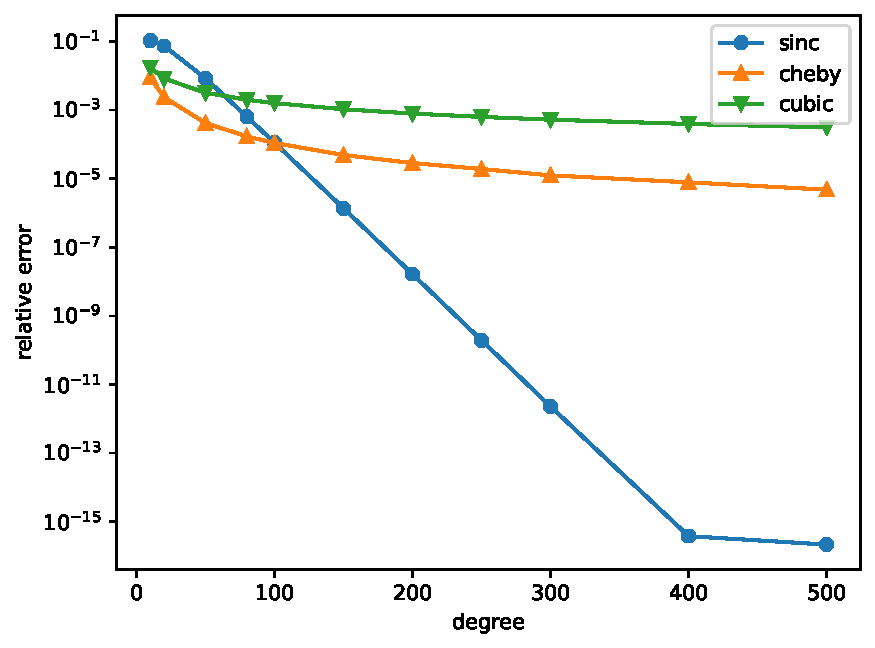
\includegraphics[width=0.3\linewidth]{ThesisFigs/sqrt_matlab.pdf}}
    \subfigure[\label{bl_matlab}Function $f(x)=e^{-10^5x}$]{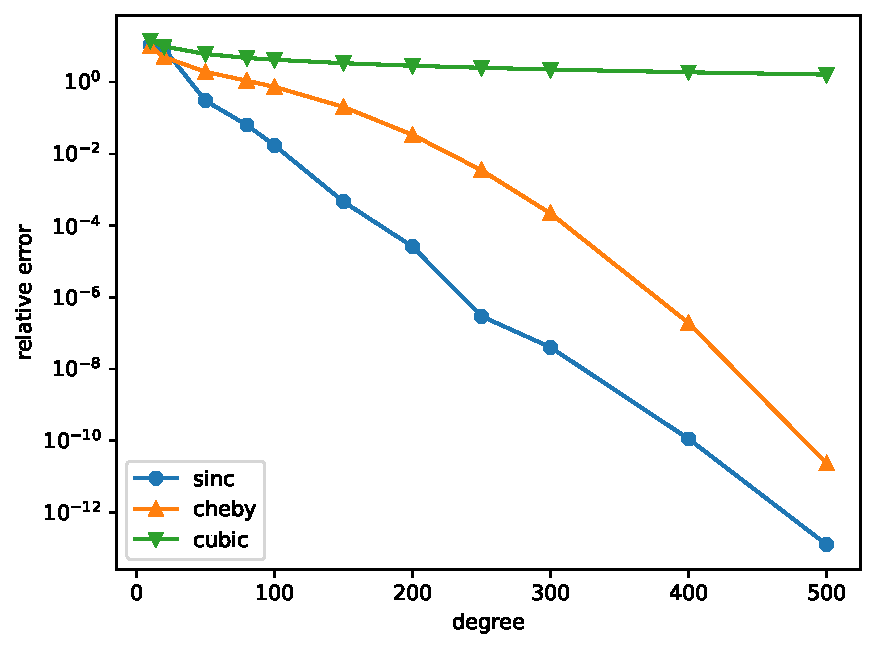
\includegraphics[width=0.3\linewidth]{ThesisFigs/bl10000_matlab.pdf}}
    \subfigure[\label{bl10000_solution}Comparative analysis of \ref{bl_matlab}]{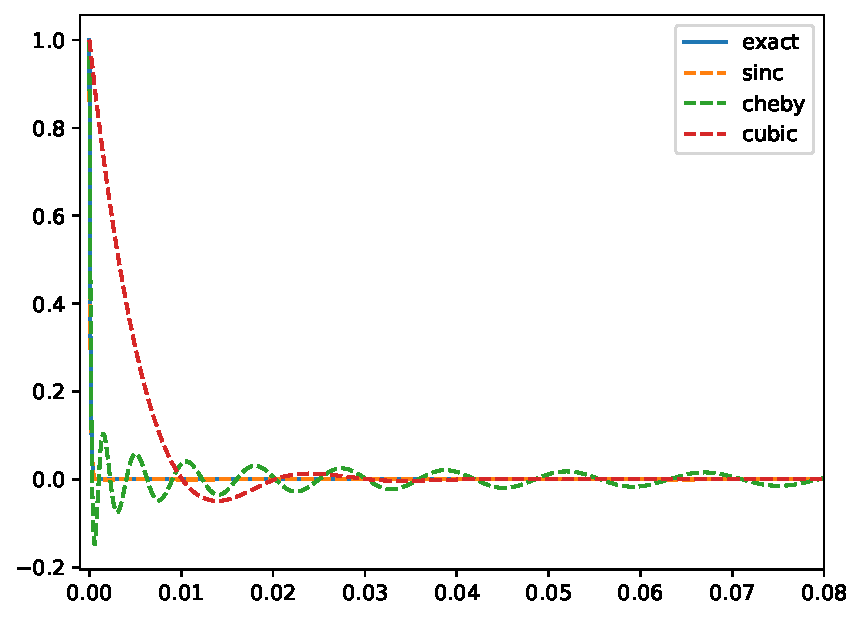
\includegraphics[width=0.3\linewidth]{ThesisFigs/bl10000_solution.pdf}}
   \caption{Comparative analysis of interpolation methods: (a) demonstrates Sinc's superior performance in handling end-point singularities, contrasting with the slower convergence of Chebyshev and spline methods; (b) illustrates exponential convergence of Sinc methods for boundary layer functions with high derivatives, while Chebyshev methods exhibit initial slow convergence; (c) presents detailed solution comparisons over $[0,0.08]$, highlighting Sinc interpolation's superior accuracy against Chebyshev's oscillatory behavior and spline's localized inaccuracies.}
    \label{fig:matlab}
\end{figure}

\subsection{Sinc Kolmogorov-Arnold Network Architecture}\label{Section: sinckan}
Consider a matrix of univariate functions $\mathbf{\Phi}=\{\phi_{p,q}\}$ where $p= 1, 2, \dots n_{in}$ and $q= 1, 2, \dots n_{out}$. The L-layer Kolmogorov-Arnold Network can be formally defined as\footnote{A comprehensive explanation of KAN architecture is provided in Appendix~\ref{Appendix: networks_kan}}:
\begin{equation}
    \mathrm{KAN} (\vx) = (\mathbf{\Phi}_{L-1} \circ \mathbf{\Phi}_{L-2} \circ \cdots \circ \mathbf{\Phi}_1 \circ \mathbf{\Phi}_0) \vx, \quad \vx\in \mathbb{R}^d.
\end{equation}

In the canonical KAN formulation \citep{liu2024kan}, each univariate function $\phi$ is approximated through a summation incorporating cubic spline interpolation:
\begin{equation}
    \phi_{\mathrm{spline}}(x)=w_b \mathrm{silu}(x)+w_s \left(\sum_i c_i B_i(x)\right),
\end{equation}
where $c_i$, $w_b$, and $w_s$ represent trainable parameters, and $B_i$ denotes the spline basis function. A natural extension to incorporate Sinc interpolation would be:
\begin{equation}\label{eq: old_sinckan}
    \phi_{\mathrm{single}}(x) = \sum_{i=-N}^N c_{i} S(i, h)(x),
\end{equation}
where $c_i$ represents trainable parameters. When $h$ is set to the optimal value given by Equation~\ref{optimal_h}, the optimal approximation of $f(x)$ in Equation~\ref{eq: sinc_approx} is achieved when $c_i^*=f(ih)$ for all $i=-N,\dots,N$. But several technical problems need to be taken into account when putting this algorithm into practice:

\paragraph{Optimal Step Size Selection}
The determination of optimal step size presents a significant challenge in machine learning frameworks, as discussed in Section~\ref{section: sinc_numerical_methods}. To address this limitation, we propose an extension to the Sinc approximation that incorporates multiple step sizes $h_j$:
\begin{equation}
    \phi_{\mathrm{multi}}(x) = \sum_{j=1}^{M}\sum_{i=-N}^N c_{i,j} S(i, h_j)(x),
\end{equation}
where $c_{i,j}$ represents the trainable parameters. Previous research \citep{stenger2012numerical} has established that step sizes larger than the optimal value predicted by Equation~\ref{optimal_h} yield improved accuracy at points distant from the origin while sacrificing precision near the origin. Conversely, smaller step sizes enhance accuracy near the origin while reducing precision at distant points. Therefore, the combination of different step sizes with adaptive weights can potentially achieve a superior approximation compared to using a single optimal step size, while eliminating the need for explicit optimal step size calculation. This expansion of the approximation through multiple step sizes $h_j$ not only circumvents the need for problem-specific step size determination but also enhances overall accuracy.

\paragraph{Coordinate Transformation Implementation}
Another significant challenge lies in the selection of appropriate coordinate transformations, which traditionally requires problem-specific optimization \citep{stenger2000summary}. Let $\mathcal{X}=\{x_i\}_{i=1}^{N}$ denote an ordered set of input points where $x_1 \leq x_2 \leq \cdots \leq x_N$. We can define the open interval $(a,b)$ as $a=x_1-\epsilon, b=x_N+\epsilon$, where $\epsilon$ represents a chosen margin, and $\xi_1=\psi^{-1}(x_1),\xi_N=\psi^{-1}(x_N)$. This transformation maps the input interval from $[x_1,x_N]$ to $[\xi_1,\xi_N]$. However, applying such transformations at each sub-layer leads to increasing and inconsistent input scales, potentially impeding network convergence \citep{ioffe2015batch}. 

To address this scaling issue, we propose that input normalization at each layer is essential. Previous research \citep{bozorgasl2024wav} has demonstrated the effectiveness of batch normalization \citep{ioffe2015batch} in enhancing KAN performance. In our SincKAN architecture, we introduce a normalizing transformation $\phi(x)=\frac{x-\mu}{\sigma}$, where $\sigma$ represents the scaling factor and $\mu$ denotes the shifting factor. The composition of $\phi$ and $\psi$ satisfies the conditions for $\psi$ specified in Theorem~\ref{Theorem: transformation}, and the transformed function $f(\psi \circ \phi^{-1}(\xi))$ maintains compliance with assumptions (1) and (2) in Theorem~\ref{Theorem: Stenger} under modified parameters $\alpha^{\star}$, $\beta^\star$, and $d^\star$ (proof provided in Appendix~\ref{Appendix: theorem 3}). Consequently, the optimal step size becomes $\sqrt{\pi d^\star/\beta^\star N}$.

We define the normalized coordinate transformation $\gamma^{-1}(x) := \phi \circ \psi^{-1}(x)$ such that $\gamma^{-1}: (a,b) \rightarrow (-\infty,\infty)$ and $[x_1,x_N] \rightarrow [\frac{\xi_1-\mu}{\sigma},\frac{\xi_N-\mu}{\sigma}]$, where $\sigma$ and $\mu$ satisfy $[\frac{\xi_1-\mu}{\sigma},\frac{\xi_N-\mu}{\sigma}] \subset [-1,1]$. This normalized transformation $\gamma$ supersedes the traditional coordinate transformation $\psi$ in our SincKAN implementation. The adaptation of optimal step size $h$ to different values of $\sigma$ and $\mu$ is facilitated by the summation of different $h_j$, allowing us to maintain consistency with the fixed scale $[-1,1]$ by defining the set $\{h_j\}$ relative to this domain, independent of specific $\sigma$ and $\mu$ values.

\paragraph{Exponential Decay Condition}
Theorem~\ref{Theorem: transformation} imposes an exponential decay condition requiring $f(-\infty)=f(+\infty)=0$. To extend Sinc methods to general functions, \citep{richardson2011sinc} proposes interpolating the difference $g-f$ rather than $f$ directly, where $g$ represents a linear function matching $f$ at the endpoints. In our SincKAN architecture, we implement this concept through a learnable linear function serving as a skip-connection for difference approximation.

Integrating these three methodological innovations, we define our learnable activation function in SincKAN as:
\begin{equation}\label{eq: Sinc activation function}
    \phi_{\mathrm{sinc}}(x) = c_1x+c_2+ \sum_{j=1}^{M}\sum_{i=-N}^N c_{i,j} S(i, h_j)(\gamma^{-1}(x)),
\end{equation}
where $c_1$, $c_2$, and $c_{i,j}$ represent learnable parameters, $S$ denotes the Sinc function, and $\gamma$ represents the normalized transformation.

\section{Experimental Validation}\label{Section: experiments}
This section presents a comprehensive evaluation of SincKAN's performance through a series of carefully designed experiments encompassing function approximation and PDE solution tasks. We compare SincKAN against several representative neural network architectures: the classical Multilayer Perceptron (MLP) commonly employed in PINNs; Modified MLP, which enhances hidden layer capability through high-dimensional feature space projection \citep{wang2021understanding}; the original KAN architecture; and ChebyKAN, which leverages Chebyshev polynomials' approximation capabilities and has been extensively validated in previous research \citep{shukla2024comprehensive}.

In our implementation, we employ the hyperbolic tangent function for the normalized transformation $\gamma(x)=\tanh(x)$ and incorporate a linear skip connection with parameters $w_1 \in \mathbb{R}^{n_{in}\times n_{out}}$ and $w_2 \in \mathbb{R}^{n_{out}}$. It is noteworthy that we observed the instability in ChebyKAN implementation previously reported by \citep{shukla2024comprehensive}; consequently, our experiments utilize the modified ChebyKAN variant proposed in their work, which incorporates a hyperbolic tangent activation function between layers. Detailed architectural specifications and hyperparameter configurations are provided in Appendices~\ref{Appendix: networks} and \ref{Appendix: expeirment details}, respectively.

\subsection{Function Approximation Analysis}
Function approximation represents a fundamental objective of KANs, with significant applications in feature identification, modular structure discovery, and symbolic formula extraction \citep{liu2024kan2}. Moreover, the neural network training process can be conceptualized as approximating mappings between complex functional spaces, making approximation accuracy a direct indicator of network capability. Therefore, we begin our experimental validation with approximation tasks to demonstrate SincKAN's competence and establish its viability as a competitive architecture. To maintain consistency with previous KAN research, we employ the Root Mean Square Error (RMSE) as our primary evaluation metric.

While Sinc numerical methods have established theoretical and empirical superiority in handling singularities, we posit that SincKAN's applicability extends beyond traditional numerical methods to general machine learning scenarios. To demonstrate this robustness, we conducted extensive experiments across both smooth functions (where cubic spline interpolation traditionally excels) and functions with singularities (where Sinc interpolation demonstrates advantages). Table~\ref{table: function approxmation} presents a subset of these results, with complete results available in Table~\ref{table: function approxmation rest}. Detailed function specifications are provided in Appendix~\ref{Appendix: details of approximate functions}.

\begin{table}[ht]
\caption{RMSE of functions for approximation}
\label{table: function approxmation}
\begin{center}
\begin{adjustbox}{width=\columnwidth, center}
\begin{tabular}{llllll}
\multicolumn{1}{c}{\bf Function name}  & \multicolumn{1}{c}{\bf MLP} & \multicolumn{1}{c}{\bf modified MLP} &\multicolumn{1}{c}{\bf KAN} & \multicolumn{1}{c}{\bf ChebyKAN} & \multicolumn{1}{c}{\bf SincKAN (ours)} 
\\ \hline 
\textit{sin-low} & $1.51 e\mbox{-}2 \pm 2.01 e\mbox{-}2$ & $7.29e\mbox{-}4 \pm 2.98 e\mbox{-}4$ & $1.27e\mbox{-}3 \pm 3.13e\mbox{-}4$ &
$1.76e\mbox{-}3 \pm 3.19e\mbox{-}4$ &
\textcolor{red}{$3.55 e\mbox{-}4 \pm 3.08 e\mbox{-}4$} \\ 
\textit{sin-high} & $7.07e\mbox{-}1 \pm 6.44e\mbox{-}8$ & $7.07 e\mbox{-}1 \pm 1.15 e\mbox{-}5$ & $7.06e\mbox{-}1 \pm 1.36e\mbox{-}3$ &
$5.70e\mbox{-}2 \pm 5.99 e\mbox{-}3$ &
\textcolor{red}{$3.94e\mbox{-}2 \pm 5.36e\mbox{-}3$} \\ 
\textit{multi-sqrt} & $2.06e\mbox{-}3 \pm 1.16e\mbox{-}3$ & $4.59e\mbox{-}4 \pm 4.86e\mbox{-}4$ & $3.61e\mbox{-}4 \pm 8.67 e\mbox{-}5$ &
$2.34e\mbox{-}3 \pm 1.17e\mbox{-}3$ &
\textcolor{red}{$2.14e\mbox{-}4 \pm 2.49 e\mbox{-}4$} \\ 
\textit{piece\mbox{-}wise} & $2.01e\mbox{-}2 \pm 5.16e\mbox{-}3$ & $3.76e\mbox{-}2 \pm 1.83e\mbox{-}2$ & $5.84e\mbox{-}2 \pm 1.03e\mbox{-}2$ &
$7.28e\mbox{-}3 \pm 9.59 e\mbox{-}4$ &
\textcolor{red}{$2.14e\mbox{-}3 \pm 7.76e\mbox{-}4$} \\ 
\textit{spectral-bias} & $4.18e\mbox{-}3 \pm 1.18 e\mbox{-}3$ & $1.59e\mbox{-}3 \pm 2.39e\mbox{-}4$ & $4.73e\mbox{-}2 \pm 9.94 e\mbox{-}3$ &
$5.60e\mbox{-}3 \pm 2.56 e\mbox{-}4$ &
\textcolor{red}{$1.48e\mbox{-}3 \pm 1.82 e\mbox{-}4$} \\
\textcolor{blue}{\textit{multimodal2-2d}} & $7.55e\mbox{-}3 \pm 2.59 e\mbox{-}3$ & $2.43e\mbox{-}3 \pm 1.15e\mbox{-}3$ & $7.97e\mbox{-}3 \pm 4.82 e\mbox{-}3$ &
$6.12e\mbox{-}2 \pm 2.02e\mbox{-}2$ &
\textcolor{red}{$2.11e\mbox{-}3 \pm 3.57e\mbox{-}4$} \\
\textcolor{blue}{\textit{fractal-2d}} & $2.89e\mbox{-}2 \pm 2.40 e\mbox{-}2$ & $2.60e\mbox{-}2 \pm 7.26e\mbox{-}3$ & $2.54e\mbox{-}1 \pm 1.88 e\mbox{-}2$ &
$6.14e\mbox{-}2 \pm 5.07e\mbox{-}3$ &
\textcolor{red}{$7.53e\mbox{-}3 \pm 6.09e\mbox{-}4$} \\
\textcolor{blue}{\textit{lpmv}} & $1.27e\mbox{-}3 \pm 6.13 e\mbox{-}5$ & $3.79e\mbox{-}4 \pm 1.58e\mbox{-}4$ & $4.19e\mbox{-}4 \pm 1.14 e\mbox{-}4$ &
$8.42e\mbox{-}3 \pm 1.29 e\mbox{-}3$ &
\textcolor{red}{$2.72e\mbox{-}4 \pm 1.97 e\mbox{-}5$} \\
\textcolor{blue}{\textit{ellipj}} & $6.51e\mbox{-}4 \pm 2.40 e\mbox{-}5$ & $7.75e\mbox{-}5 \pm 9.74e\mbox{-}7$ & $1.29e\mbox{-}4 \pm 2.00 e\mbox{-}5$ &
$4.80e\mbox{-}3 \pm 4.03 e\mbox{-}4$ &
\textcolor{red}{$3.02e\mbox{-}5 \pm 5.08 e\mbox{-}6$} \\
\textcolor{blue}{\textit{exp-sin-4d}} & $3.85e\mbox{-}2 \pm 5.27 e\mbox{-}4$ & $1.53e\mbox{-}2 \pm 1.33e\mbox{-}3$ & $6.22e\mbox{-}3 \pm 1.23 e\mbox{-}3$ &
$4.96e\mbox{-}1 \pm 1.91e\mbox{-}2$ &
\textcolor{red}{$2.74e\mbox{-}3 \pm 3.29e\mbox{-}4$} \\
\textcolor{blue}{\textit{exp-100d}} & $3.99e\mbox{-}3 \pm 1.88 e\mbox{-}4$ & $1.04e\mbox{-}1 \pm 4.96e\mbox{-}4$ & $9.42e\mbox{-}2 \pm 3.02 e\mbox{-}3$ &
$nan$ &
\textcolor{red}{$2.91e\mbox{-}3 \pm 1.03 e\mbox{-}5$} \\
\end{tabular}
\end{adjustbox}
\end{center}
\end{table}
The experimental results demonstrate SincKAN's exceptional performance across diverse function classes, including low-frequency functions (\textit{sin-low}), high-frequency functions (\textit{sin-high}), continuous but non-differentiable functions (\textit{multi-sqrt}), and discontinuous functions (\textit{piece-wise}). Particularly noteworthy is SincKAN's performance on the \textit{spectral-bias} function, specifically designed to evaluate networks' ability to address the spectral bias phenomenon identified by \citep{rahaman2019spectral}. The results indicate that SincKAN achieves substantial mitigation of spectral bias compared to alternative architectures.

\begin{figure}[ht]
    \centering
    \subfigure[\label{piecewise_solution}]{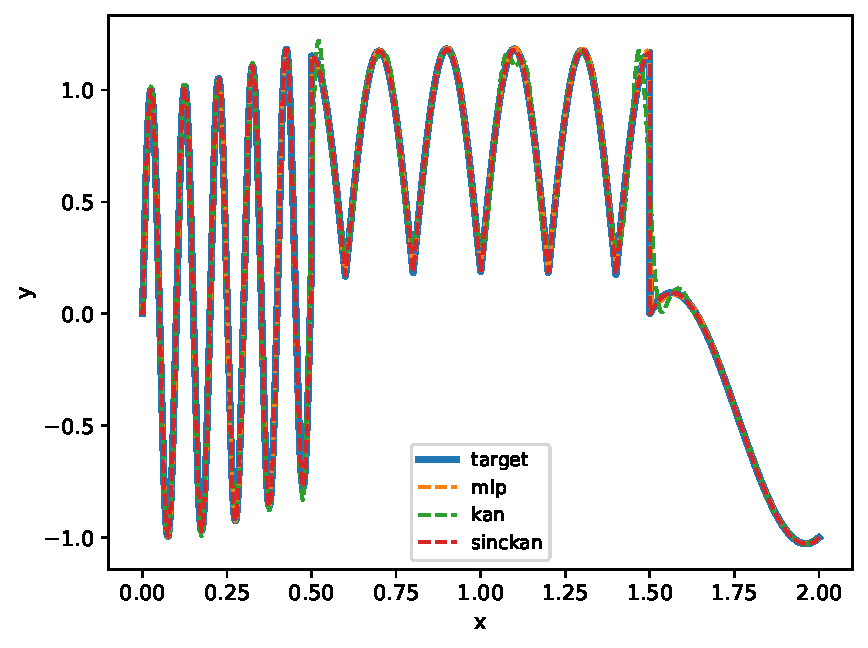
\includegraphics[width=0.3\linewidth]{ThesisFigs/piecewise.pdf}}
    \subfigure[\label{piecewise_error}]{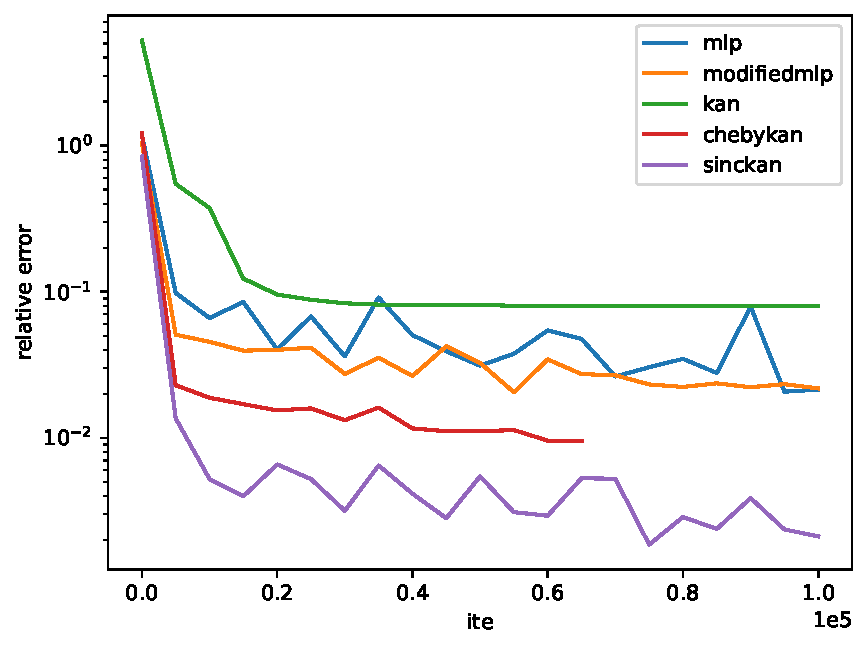
\includegraphics[width=0.3\linewidth]{ThesisFigs/piecewise_error.pdf}}\\
    \subfigure[\label{piecewise_sub1}]{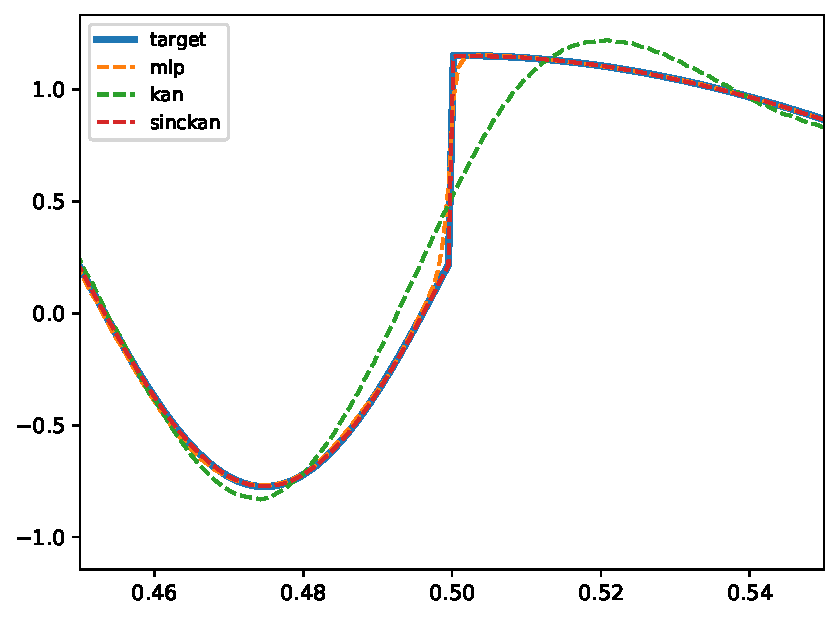
\includegraphics[width=0.3\linewidth]{ThesisFigs/piecewise_sub1.pdf}}
    \subfigure[\label{piecewise_sub2}]{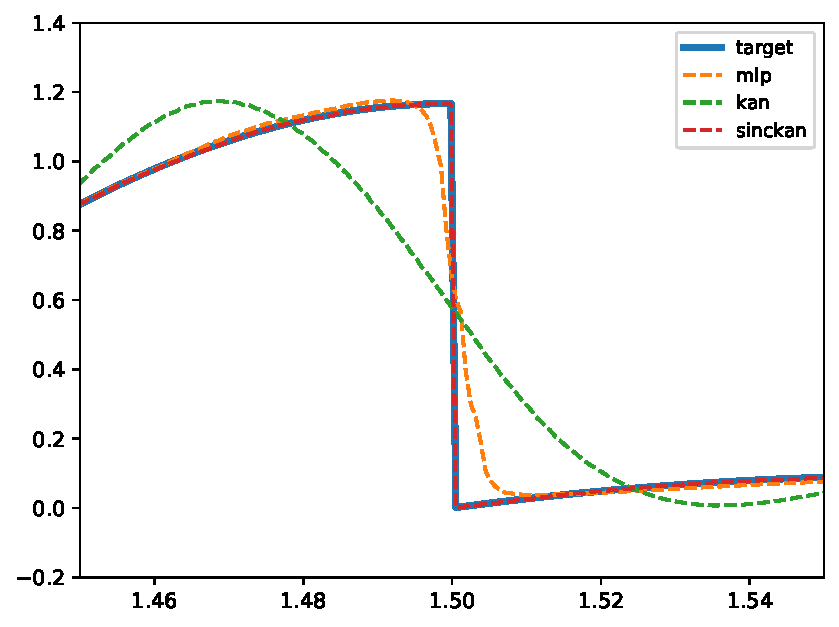
\includegraphics[width=0.3\linewidth]{ThesisFigs/piecewise_sub3.pdf}}
    \caption{\cref{piecewise_solution} depicts the function of \textit{piece-wise} in \cref{table: function approxmation} and compares the performance of SincKAN with MLP and KAN. \cref{piecewise_error} demonstrates the convergence of relative error for all networks, note that although the ChebyKAN we used is the modified ChebyKAN, its training is still unstable. Herein, the results of ChebyKAN in this paper are always the last valid error. \cref{piecewise_sub1} and \cref{piecewise_sub2} demonstrate the singularities in detail and show that the SincKAN can approximate the singularities well while MLP and KAN have obvious differences.}
    \label{fig:enter-label}
\end{figure}
\subsubsection{Step Size Selection Analysis}
The implementation of multiple step sizes $\{h_i\}$ represents a novel methodological contribution specific to SincKAN architecture. To evaluate the efficacy of this approach, we conducted a comprehensive experimental analysis. Let $h_{min}=\min \{h_i\}$ and $h_{max}=\max \{h_i\}$ denote the bounds of the step size range. Based on the theoretical framework presented in Section~\ref{Section: sinckan}, optimal performance should be achieved when the theoretical optimal step size $h^*=\sqrt{\pi d^\star/\beta^\star N}$ lies within the interval $(h_{min}, h_{max})$. 

Our experimental design incorporates two distinct step size sequence formulations, each parameterized by base value $h_0$ and cardinality $M$:

\begin{enumerate}
    \item Inverse decay sequence: $\{h_i\}_{i=1}^{M}$ where $h_i=1/ih_0$
    \item Exponential decay sequence: $\{h_i\}_{i=1}^{M}$ where $h_i=1/h_0^i$
\end{enumerate}

The experimental protocol involved training SincKAN on two representative functions: \textit{sin-low} and \textit{sin-high}. For the inverse decay sequence, we examined $M \in \{1,6,12,24\}$, while the exponential decay sequence was evaluated with $M \in \{1,2,3\}$. Both sequences were tested across base values $h_0 \in \{2.0, \pi, 6.0, 10.0\}$. The number of discretization points $N_{points}$ and degree $N_{degree}$ (where $N_{degree}=2N+1$, with $N$ defined in Equation~\ref{eq: Sinc activation function}) significantly influence SincKAN's performance under different step size configurations. For this analysis, we empirically set $N_{degree}=100$ and $N_{points}=5000$.

The results are illustrated in \cref{fig:select_h_inverse} for inverse decay and \cref{fig:select_h_exp} for exponential decay, and the details including the corresponding error bars are shown in \cref{Appendix: select_h}. For the \textit{sin-low} function, optimal performance (RMSE = $1.49 \times 10^{-4} \pm 8.74 \times 10^{-5}$) was achieved with $h_0=10.0$ and $M=1$. In contrast, the \textit{sin-high} function exhibited superior performance (RMSE = $4.60 \times 10^{-3} \pm 3.70 \times 10^{-4}$) under inverse decay with $h_0=10.0$ and $M=24$. While these functions, characterized by distinctly different Fourier spectra ($4\pi$ and $400\pi$ respectively), yielded divergent optimal hyperparameter configurations, notably accurate approximations for both functions were achieved using inverse decay with $M=6$ and $h_0=10.0$. We also discuss the relationship between degree and data size in \cref{Appendix: scaling law} and the update of basis in \cref{Appendix: update}.

\subsection{Physics-Informed Neural Network Implementation}
The solution of partial differential equations represents a cornerstone of scientific computing, with PINNs emerging as a prominent framework for neural network-based PDE solutions. We demonstrate SincKAN's capabilities through a series of challenging PDE problems. Initial validation involved a selection of classical PDEs to establish SincKAN's robustness, with results presented in Table~\ref{table:pikan_pde}. Detailed problem specifications are provided in Appendix~\ref{Appendix: details of pde}.

\begin{table}[ht]
\caption{Relative L2 error for chosen PDE problems}
\label{table:pikan_pde}
\begin{center}
\begin{adjustbox}{width=\columnwidth, center}
\begin{tabular}{llllll}
\multicolumn{1}{c}{\bf Experiments}  & \multicolumn{1}{c}{\bf MLP} & \multicolumn{1}{c}{\bf modified MLP} &\multicolumn{1}{c}{\bf KAN} & \multicolumn{1}{c}{\bf ChebyKAN} & \multicolumn{1}{c}{\bf SincKAN (ours)} 
\\ \hline  
\textit{perturbed} & $2.89e\mbox{-}2\pm 3.09e\mbox{-}2$ & $6.30e\mbox{-}1\pm1.14e\mbox{-}1$ &  $4.48e\mbox{-}3 \pm 4.20e\mbox{-}3 $& $6.73e\mbox{-}1 \pm 1.02e\mbox{-}1 $& \color{red}{$1.88e\mbox{-}3 \pm 8.55e\mbox{-}4$} \\ 
\textit{nonlinear} & $3.92e\mbox{-}1 \pm 2.36e\mbox{-}5$ & $1.56e\mbox{-}2 \pm 2.10e\mbox{-}2$ & \color{red}{$6.15e\mbox{-}4 \pm 7.96e\mbox{-}4$} & $7.78e\mbox{-}1 \pm 2.67e\mbox{-}2$  & $1.77e\mbox{-}3 \pm 1.06e\mbox{-}3$ \\ 
\textit{bl-2d} & $2.38e\mbox{-}1\pm6.22e\mbox{-}2$ & $5.34e\mbox{-}2 \pm 1.91e\mbox{-}2$ &$1.19e\mbox{-}2 \pm 4.22e\mbox{-}3$ & $5.97e\mbox{-}2\pm 3.83e\mbox{-}2$ & \color{red}{$2.31e\mbox{-}3\pm7.10e\mbox{-}4$} \\
\textit{ns-tg-u} & $8.14e\mbox{-}5 \pm 1.96e\mbox{-}6$ & \color{red}{$2.14e\mbox{-}5 \pm 2.67e\mbox{-}6$} & $3.21e\mbox{-}4 \pm 2.02e\mbox{-}5$ & $6.43e\mbox{-}2 \pm 2.70e\mbox{-}2$& $6.51e\mbox{-}4 \pm 7.03e\mbox{-}5$\\      
\textit{ns-tg-v} & $8.30e\mbox{-}5 \pm 2.47e\mbox{-}6$ & \color{red}{$1.91e\mbox{-}5 \pm 1.63e\mbox{-}6$} & $4.04e\mbox{-}4 \pm 1.25e\mbox{-}4$ & $5.86e\mbox{-}2 \pm 4.15e\mbox{-}2$& $1.34e\mbox{-}3 \pm 4.38e\mbox{-}4$
\end{tabular}
\end{adjustbox}
\end{center}
\end{table}

\begin{figure}[ht]
  \centering
  \subfigure[\label{bl_solution_sinckan}Solution comparison]{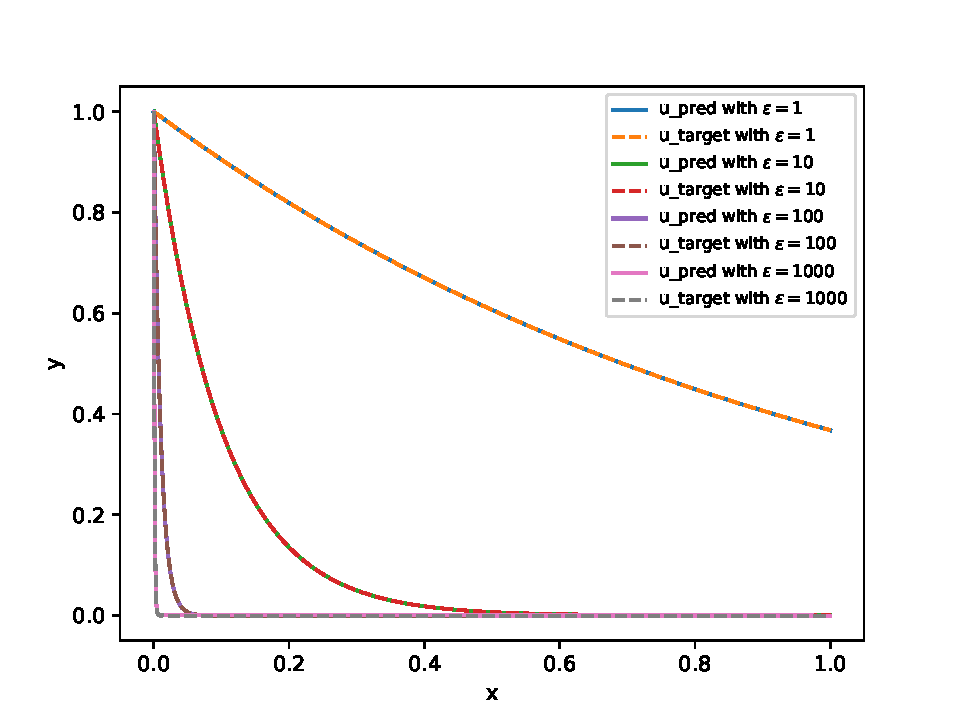
\includegraphics[width=0.3\linewidth]{ThesisFigs/bl_solution_sinckan.pdf}}
  \subfigure[\label{bl_loss_sinckan}Loss convergence]{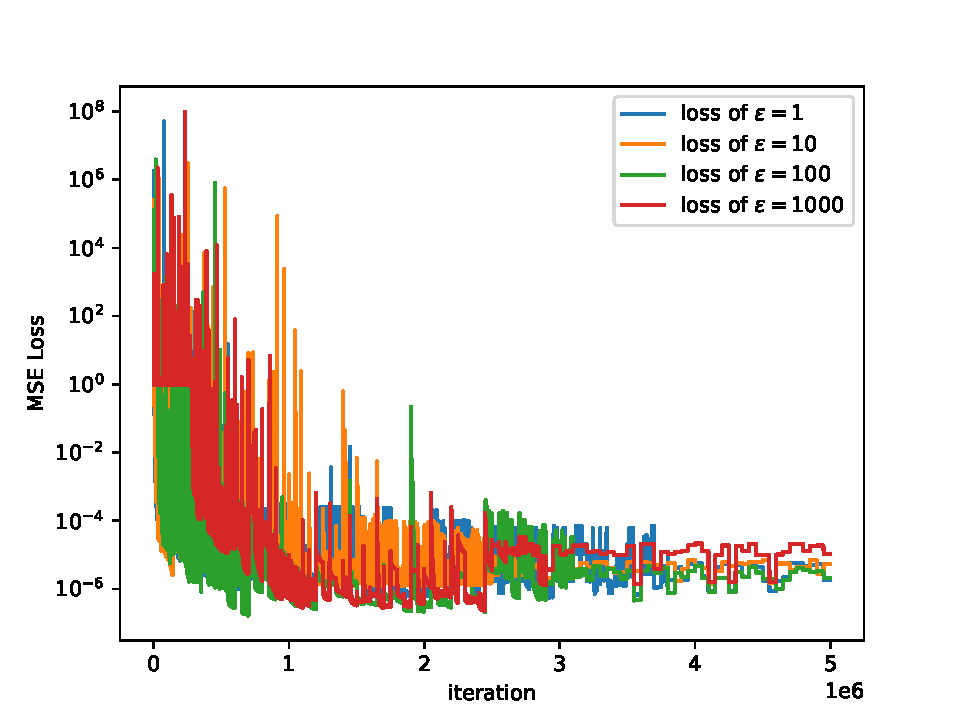
\includegraphics[width=0.3\linewidth]{ThesisFigs/bl_loss_sinckan.pdf}}
  \subfigure[\label{bl_1000_sinckan}High-$\epsilon$ performance]{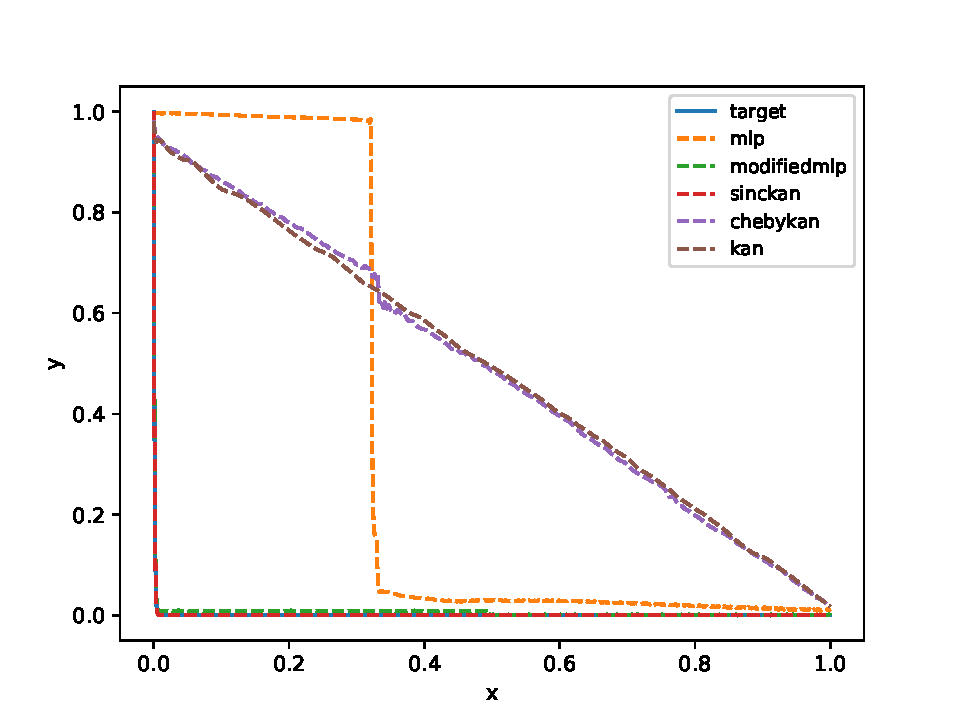
\includegraphics[width=0.3\linewidth]{ThesisFigs/bl_1000_sinckan.pdf}}
  \caption{Analysis of boundary layer problem: (a) Comparison between exact solutions and SincKAN predictions for various $\epsilon$ values, demonstrating robust performance even with extremely narrow boundary layers; (b) Training loss convergence patterns across different $\epsilon$ values; (c) Comparative performance analysis for $\epsilon=1000$, illustrating superior SincKAN performance in cases where traditional architectures struggle with large derivatives in the boundary layer.}
  \label{fig:bl_sinckan}
\end{figure}

\subsubsection{Analysis of Boundary Layer Problems}
To provide a comprehensive demonstration of SincKAN's capabilities relative to existing architectures, we conducted an in-depth analysis of the boundary layer problem:
\begin{equation} \label
{eq: bl}
u_{xx}/\epsilon+u_{x}=0, \quad x \in
 [0,1]
\end{equation}
with exact solution $u(x)=\exp (-\epsilon x)$. The parameter $\epsilon$ controls the width of the boundary layer, with increasing values of $\epsilon$ corresponding to decreasing boundary layer width and consequently increasing learning complexity. Table~\ref{table:bl_pikan} presents a comparative analysis across different values of $\epsilon$, while Figure~\ref{fig:bl_sinckan}
 provides detailed visualization of the results.

\begin{table}[ht]
\caption{Relative L2 error for different $\epsilon$ in \cref{eq: bl}}
\label{table:bl_pikan}
\begin{center}
\begin{adjustbox}{width=\columnwidth, center}
\begin{tabular}{llllll}
\multicolumn{1}{c}{\bf $\epsilon$ } & \multicolumn{1}{c}{\bf MLP} & \multicolumn{1}{c}{\bf Modified MLP} &\multicolumn{1}{c}{\bf KAN} &\multicolumn{1}{c}{\bf ChebyKAN} & \multicolumn{1}{c}{\bf SincKAN (ours)} 
\\ \hline 
1    & $ 6.60e\mbox{-}5 \pm 1.91e\mbox{-}5 $ &$ 3.88e\mbox{-}6 \pm 7.22e\mbox{-}7 $   & $ 5.97e\mbox{-}6 \pm 5.24e\mbox{-}6 $ & \color{red}{$ 1.98e\mbox{-}6 \pm 4.51e\mbox{-}7 $} & $ 7.78e\mbox{-}5 \pm 1.14e\mbox{-}4 $ \\
10   & $ 2.83e\mbox{-}4 \pm 4.22e\mbox{-}5 $& $ 1.69e\mbox{-}4 \pm 6.85e\mbox{-}5 $ &$ 3.23e\mbox{-}5 \pm 1.81e\mbox{-}5 $ & \color{red}{$4.45e\mbox{-}6 \pm 4.01e\mbox{-}7$} & $1.14e\mbox{-}4 \pm 1.64e\mbox{-}4 $\\
$10^2$  & $ 1.29e\mbox{-}3 \pm 3.24e\mbox{-}4 $& $ 6.25e\mbox{-}4 \pm 2.27e\mbox{-}4 $ & $ 1.25e\mbox{-}2 \pm 2.62e\mbox{-}3 $ & $ 5.27e\mbox{-}4 \pm 6.55e\mbox{-}4 $& \color{red}{$1.68e\mbox{-}4 \pm 6.16e\mbox{-}5$} \\
$10^3$ &$ 9.87 \pm 8.70 $ & $ 1.53e\mbox{-}1 \pm 5.59e\mbox{-}2 $    & $ 11.3 \pm 8.79 $ & $ 10.9 \pm 7.18 $ & \color{red}{$5.48e\mbox{-}3 \pm 3.45e\mbox{-}3$}\\
\textcolor{blue}{$10^4$} &$ 8.41 \pm 3.64 $ & $ 6.52 \pm 4.35 $    & $ 9.73 \pm 8.77 $ & $ 22.1 \pm 4.49 $ & \color{red}{$5.27e\mbox{-}3 \pm 1.29e\mbox{-}3$}
\end{tabular}
\end{adjustbox}
\end{center}
\end{table}

\subsubsection{Analysis of Fractional PDEs}
Fractional partial differential equations present significant computational challenges, with traditional numerical methods still struggling to address their non-local nature and inherent singularities. We examine the fractional PDE:
\begin{equation}
    -\Delta^su+\gamma u=f, \quad x\in
 (-1,1),
\end{equation}
where $f=1+\gamma u$
, with solution:
\begin{equation}
    u(x)=\frac{2^{-2s}\Gamma(d/2)}{\Gamma(d/2+s)\Gamma(1+s)}(1-\|x\|
^2_2)^s.
\end{equation}

Figure~\ref{fig:frac}
 presents our comparative analysis results. The superior performance of SincKAN in handling the inherent singularities of fractional PDEs is particularly evident in the convergence patterns and error distributions.

\begin{figure}[ht]
  \centering
  \subfigure[\label{frac_loss}Loss convergence]{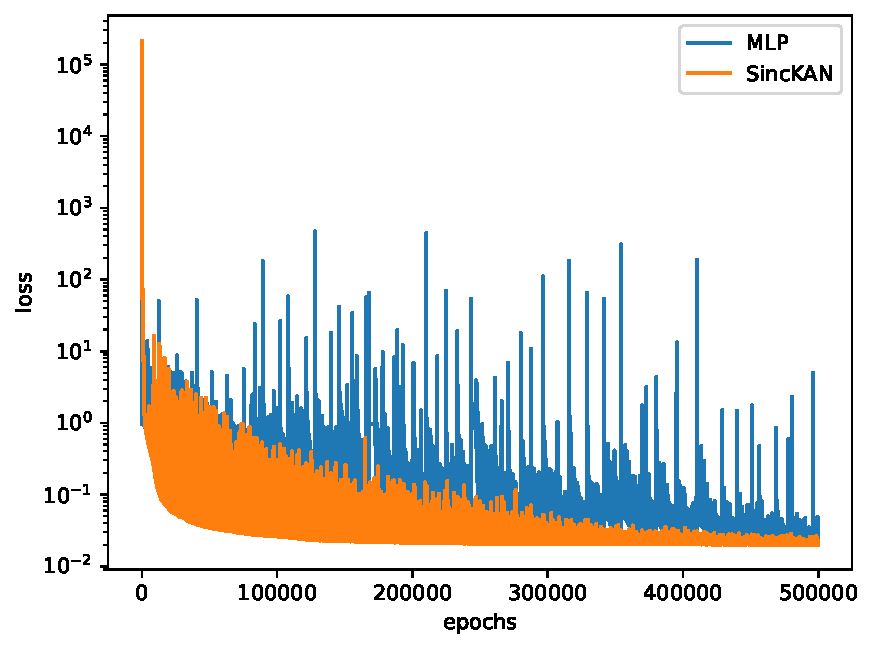
\includegraphics[width=0.3\linewidth]{ThesisFigs/frac_loss85_1.pdf}}
  \subfigure[\label{frac_error85}Error analysis ($s=0.85$)]{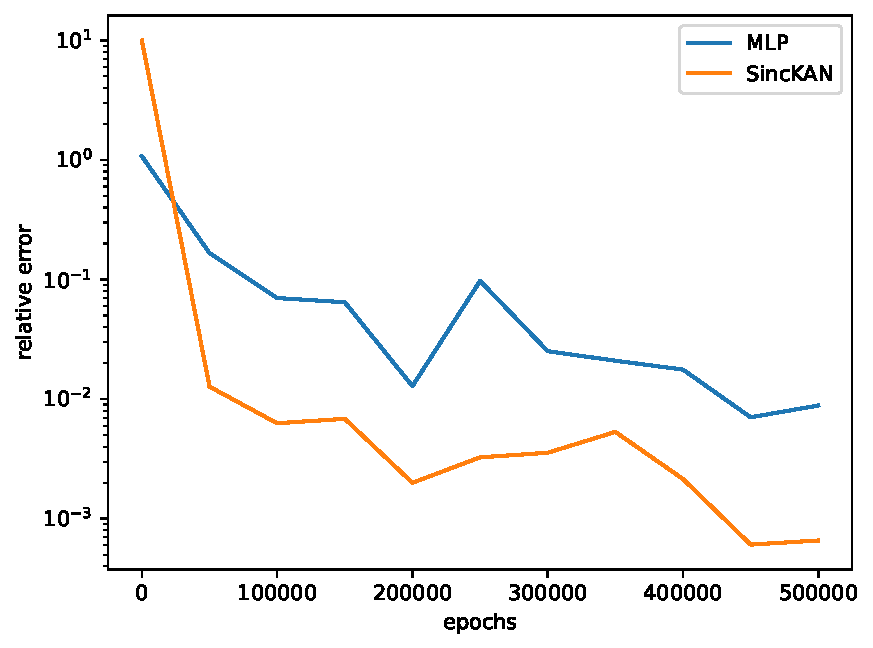
\includegraphics[width=0.3\linewidth]{ThesisFigs/frac_error85_1.pdf}}
  \subfigure[\label{frac_error95}Error analysis ($s=0.95$)]{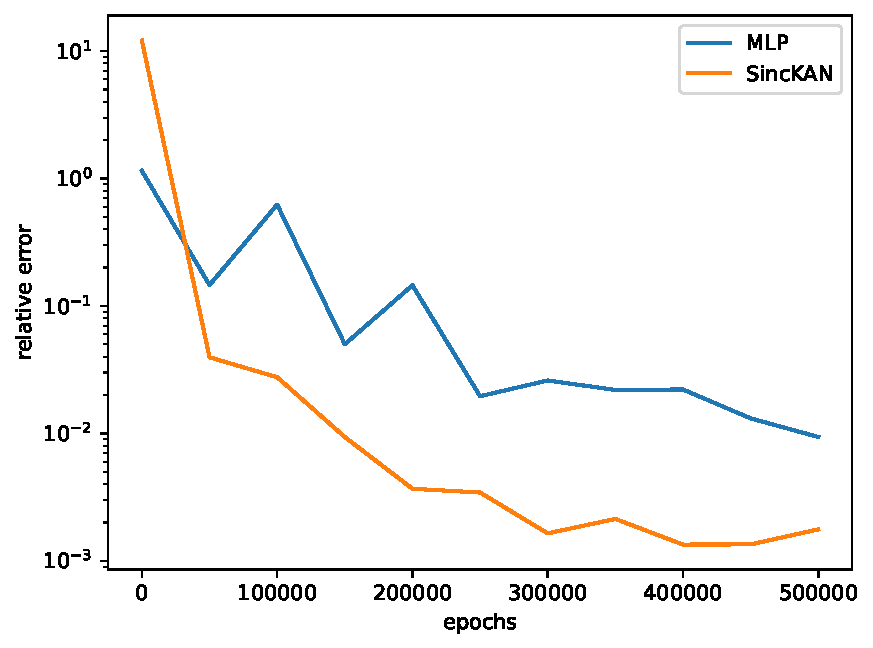
\includegraphics[width=0.3\linewidth]{ThesisFigs/frac_error95_1.pdf}}
  \caption{Fractional PDE analysis: (a) Comparative loss convergence between MLP and SincKAN for $s=0.85$; (b,c) Error distribution analysis for $s=0.85$ and $s=0.95$ respectively, demonstrating SincKAN's superior handling of fractional-order derivatives.}
  \label{fig:frac}
\end{figure}

\subsubsection{High-Dimensional Problem Analysis}
To evaluate scalability, we examined the classical high-dimensional Poisson equation:
\begin{equation}
    \Delta u =f, \quad \boldsymbol{x}\in
 [0,1]^d,
\end{equation}
with source term $f=2\alpha(2\alpha \|\boldsymbol{x}\|^2_2-d) e^{-\alpha \|\boldsymbol{x}\|_2^2}$, yielding the exact solution $u(\boldsymbol{x})=e^{-\alpha \|\boldsymbol{x}\|^2_2}$. Our experiments focused on the challenging case of $d=100$ dimensions, with detailed experimental parameters provided in Appendix~\ref{Appendix: expeirment details}
.

\begin{figure}[ht]
  \centering
  \subfigure[\label{high_distribution}Point distribution]{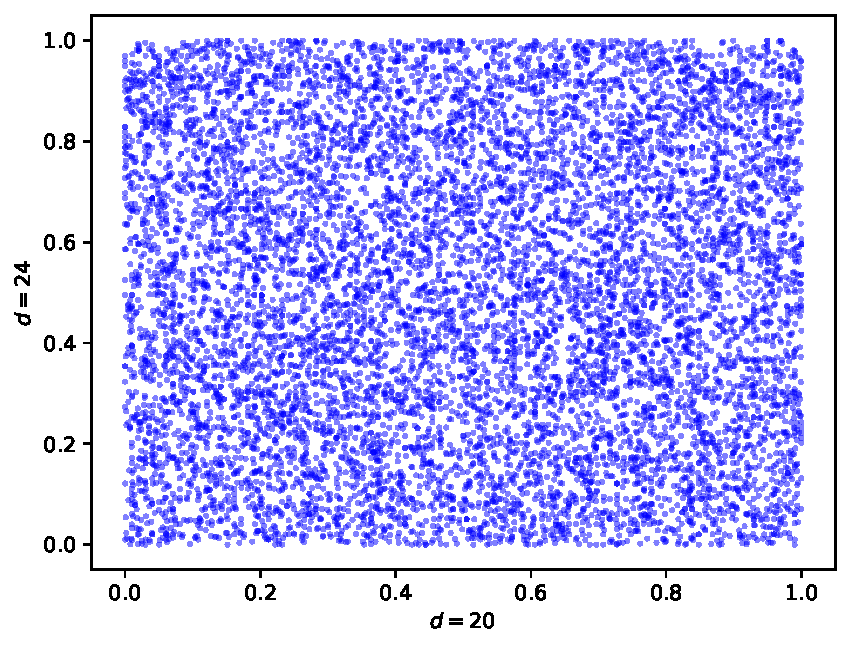
\includegraphics[width=0.3\linewidth]{ThesisFigs/points_distribution.pdf}}
  \subfigure[\label{high_mlp}MLP error analysis]{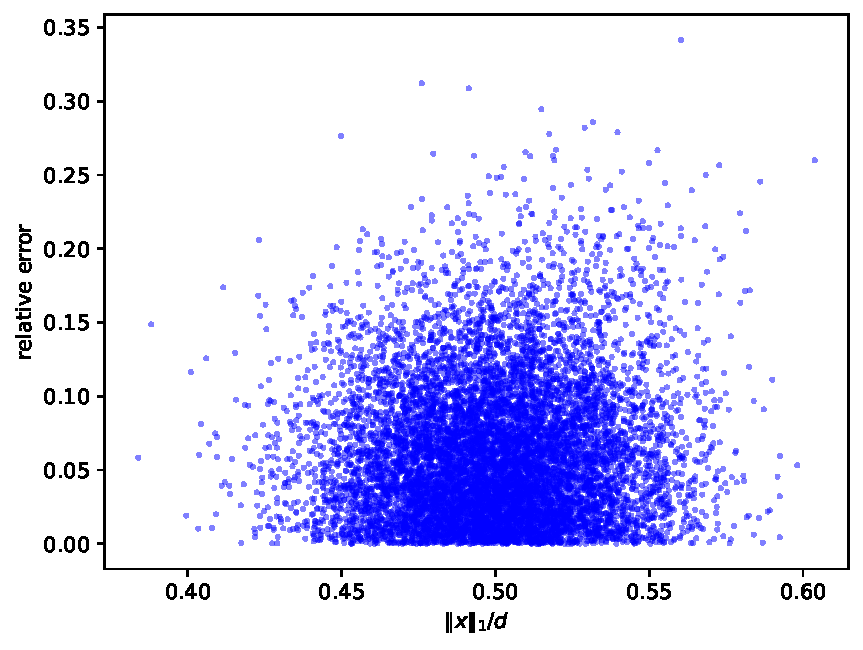
\includegraphics[width=0.3\linewidth]{ThesisFigs/high-dim_mlp.pdf}}
  \subfigure[\label{high_sinckan}SincKAN error analysis]{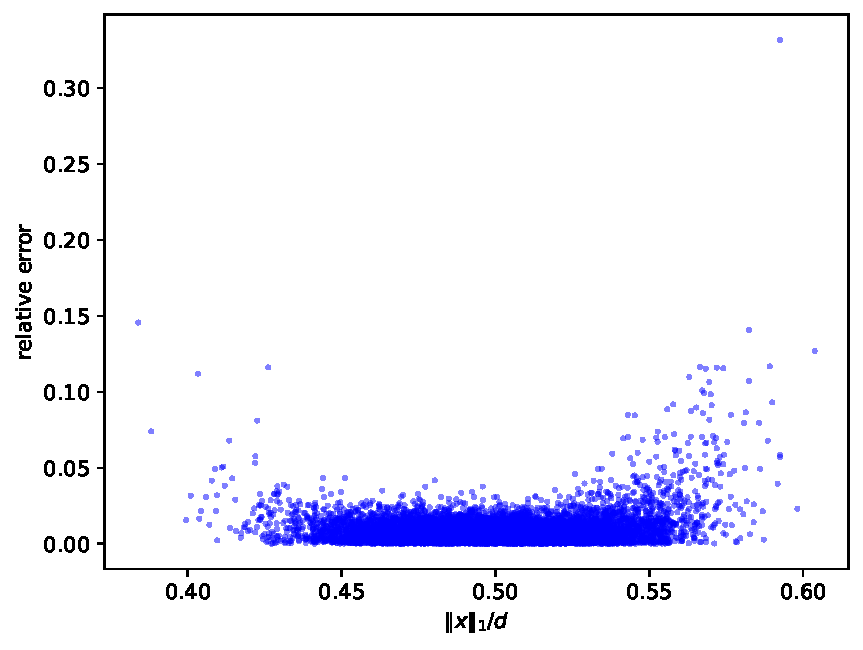
\includegraphics[width=0.3\linewidth]{ThesisFigs/high-dim_sinckan.pdf}}
  \caption{High-dimensional analysis: (a) Distribution visualization of test points in dimensions 20 and 24; (b,c) Comparative error analysis between MLP and SincKAN implementations, demonstrating SincKAN's superior performance in high-dimensional spaces.}
  \label{fig:high_dim}
\end{figure}

\subsubsection{Ablation Studies}
To systematically evaluate the architectural contributions of SincKAN, we conducted comprehensive ablation studies examining two key components: the normalized transformation and the linear skip connection. While Sinc numerical methods traditionally employ various coordinate transformations, and KANs incorporate skip connections with SiLU functions, our implementation introduces specific modifications to these elements. To rigorously assess the impact of these modifications, we performed comparative analyses using two representative test cases: Burger's equation (Equation~\ref{eq:burgers}) and the time-dependent nonlinear equation (Equation~\ref{eq:tnonlinear}
).

\begin{table}[ht]
\caption{Relative L2 error for ablation study}
\label{table:ablation}
\begin{center}
\begin{adjustbox}{width=0.5\columnwidth, center}
\begin{tabular}{ccccll}
\multicolumn{1}{c} {$\psi$}  & \multicolumn{1}{c}{$\gamma$} & \multicolumn{1}{c}{\bf Linear }  &\multicolumn{1}{c}{\bf SiLU} & \multicolumn{1}{c}{\bf T-nonlinear} & \multicolumn{1}{c}{\bf Burgers' equation}
\\ \hline  
\ding{56} & \ding{56} & \ding{56} & \ding{56} & $9.20e\mbox{-}4\pm4.31e\mbox{-}4$ & $1.57e\mbox{-}2\pm4.31e\mbox{-}3$\\
\ding{56} & \ding{52} & \ding{56} & \ding{56} &  $5.80e\mbox{-}4\pm1.89e\mbox{-}4$ &\color{red}{$6.21e\mbox{-}4\pm1.96e\mbox{-}4$}\\
\ding{56} & \ding{52} & \ding{52} & \ding{56} & $2.44e\mbox{-}4\pm6.08e\mbox{-}5$ & $3.12e\mbox{-}3\pm2.48e\mbox{-}3$ \\
\ding{56} & \ding{52} & \ding{56} & \ding{52} & \color{red}{$1.60e\mbox{-}4\pm3.17e\mbox{-}5$} & $8.90e\mbox{-}3\pm6.76e\mbox{-}3$ \\
\ding{52} & \ding{56} & \ding{52} & \ding{56} & $1.11e\mbox{-}2\pm1.17e\mbox{-}3$& $7.36e\mbox{-}2\pm2.02e\mbox{-}2$ \\
\ding{52} & \ding{56} & \ding{56} & \ding{52} & $1.30e\mbox{-}2\pm4.00e\mbox{-}4$ & $1.12e\mbox{-}1\pm6.80e\mbox{-}3$ \\
\end{tabular}
\end{adjustbox}
\end{center}
\end{table}

Table~\ref{table:ablation} presents our ablation study results, where $\psi(x)=\log(\frac{x-a}{b-x})$ represents the traditional transformation, $\gamma(x)=\tanh(x)$ denotes our normalized transformation, $\mathrm{Linear}(x)=w_1x+w_2+\phi(x)$ represents the linear skip connection, and $\mathrm{SiLU}(x)=w_b\mathrm{silu}(x)+w_s\phi(x)$
 indicates the SiLU skip connection. The results reveal several significant findings:

First, the non-normalized transformation consistently demonstrates inferior performance compared to configurations without transformations, highlighting the importance of proper normalization in neural network architectures. Second, while the linear skip connection may not achieve optimal performance for both equations individually, it exhibits superior stability characteristics in the SincKAN framework, suggesting its value as a robust architectural component.

\section{Conclusion}\label{Section: conclusion}
This research introduces Sinc Kolmogorov-Arnold Networks (SincKANs), a novel neural network architecture that leverages the powerful approximation capabilities of Sinc functions within the KAN framework. By implementing Sinc functions for activation function interpolation, SincKANs inherit and enhance the ability to handle singularities effectively. To address the challenges of optimal step size selection, we introduced multi-$h$
 interpolation, which our experimental results indicate is fundamental to SincKAN's superior performance in approximating complex smooth functions.

The implementation challenges were systematically addressed through three key innovations: (1) the introduction of normalized transformation to prevent convergence issues, (2) the implementation of skip-connections with learnable linear functions to satisfy decay conditions, and (3) the development of multi-step size interpolation methodology. These modifications collectively enable SincKANs to serve as a competitive alternative to existing neural network architectures in the PINN framework.

Our experimental validation began with function approximation tasks, where SincKANs demonstrated superior performance across diverse test cases. However, we acknowledge that direct function approximation rarely represents the primary objective in machine learning applications. Following this validation, we evaluated SincKAN performance in PDE solution tasks within the PINN framework. While SincKANs achieved impressive approximation accuracy across all tested PDEs, their optimal performance was particularly evident in boundary layer problems, though some oscillation effects were observed due to derivative approximation challenges.

\textbf{Limitations}: The accuracy of derivative approximation using Sinc numerical methods exhibits inherent limitations near Sinc end-points. While various solutions have been proposed in the literature, such as Lagrange polynomial approximation \citep{stenger2009polynomial} and discrete function substitution \citep{wu2006sinc}, these approaches have not yet been successfully adapted to the SincKAN architecture for PINN applications. To mitigate accuracy issues, we employed conservative parameter settings ($h_0$, $M$, and $N$), which, while enabling successful PDE solution, potentially limit SincKAN's full capabilities (detailed oscillation analysis provided in Appendix~\ref{Appendix: oscillation}
). These limitations particularly affect high-order problems such as Korteweg–De Vries and Kuramoto–Sivashinsky equations.

\textbf{Future Directions}: Several promising research directions emerge from our findings. For PDEs requiring only first derivatives, SincKAN can potentially utilize larger parameter values ($h_0$, $M$, and $N$), potentially improving performance. The mixed residual method approach of MIM \citep{lyu2022mim,li2024priori}, which transforms high-order PDEs into first-order PDE systems, presents a promising avenue for extending SincKAN capabilities to higher-order problems. Additionally, alternative differentiation approaches \citep{cen2024deep,yu2024fourier}
 warrant investigation as potential replacements for automatic differentiation in the SincKAN framework.

% ------------------------------------------------------------------------

%%% Local Variables: 
%%% mode: latex
%%% TeX-master: "../thesis"
%%% End: 

% \chapter{My Third Chapter}
% \ifpdf
%     \graphicspath{{Chapter3/Chapter3Figs/PNG/}{Chapter3/Chapter3Figs/PDF/}{Chapter3/Chapter3Figs/}}
% \else
%     \graphicspath{{Chapter3/Chapter3Figs/EPS/}{Chapter3/Chapter3Figs/}}
% \fi

% \section{First Section of the Third Chapter}
% \markboth{\MakeUppercase{\thechapter. My Third Chapter }}{\thechapter. My Third Chapter}
% And now I begin my third chapter here ...

% \subsection{first subsection in the First Section}
% ... and some more 

% \subsection{second subsection in the First Section}
% ... and some more ...

% \subsubsection{first subsub section in the second subsection}
% ... and some more in the first subsub section otherwise it all looks the same
% doesn't it? well we can add some text to it ...

% \subsection{third subsection in the First Section}
% ... and some more ...

% \subsubsection{first subsub section in the third subsection}
% ... and some more in the first subsub section otherwise it all looks the same
% doesn't it? well we can add some text to it and some more and some more and
% some more and some more and some more and some more and some more ...

% \subsubsection{second subsub section in the third subsection}
% ... and some more in the first subsub section otherwise it all looks the same
% doesn't it? well we can add some text to it ...

% \section{Second Section of the Third Chapter}
% \markboth{\MakeUppercase{\thechapter. My Third Chapter }}{\thechapter. My Third Chapter}
% and here I write more ...

\chapter{Research plan for PhD thesis}

\section{Extension of SincKAN}

\subsection{Strengths and weaknesses of SincKAN: a reflection from ICLR 2025 Conference Formal Reviews}

Our early-stage work, \textbf{"Sinc Kolmogorov-Arnold Network and Its Applications on Physics-Informed Neural Networks"}, was submitted to the \textit{Thirteenth International Conference on Learning Representations (ICLR 2025 Conference)} on October 1, 2024. ICLR is among the top three machine learning conferences and is a premier gathering of industrial and academic professionals dedicated to the branch of artificial intelligence generally referred to as deep learning.

Based on feedback from four ICLR reviewers, we summarize the strengths of SincKAN as follows:
\begin{enumerate}
    \item \textbf{Superior Performance:} Compared to other state-of-the-art deep learning models, SincKAN demonstrates superior performance in approximating functions and solving PDEs with singularities. Additionally, SincKAN achieves near-SOTA performance across various computational cases, ranging from one dimension to 100 dimensions.
    \item \textbf{Innovation and Range Expansion:} SincKAN broadens the application range, enhances the accuracy, and introduces novelty to the Kolmogorov-Arnold Network by replacing cubic splines with Sinc interpolants.
    \item \textbf{Theoretical Guarantees:} Theorems presented in \cref{Theorem: Stenger} and \cref{Theorem: transformation} offer theoretical guarantees for the convergence and accuracy of SincKAN. Furthermore, the Multi-h approach provides an effective strategy to address the challenge of selecting the optimal step size.

\end{enumerate}

At the same time, some criticisms exist regarding the limitations of SincKAN:
    \begin{enumerate}
    \item \textbf{Limited Scope of Computational Cases:} Some reviewers noted that most numerical experiments focus on one-dimensional function fitting and PDE solution fitting. The functions and PDEs tested are somewhat artificial and simplistic, lacking the complexity and irregular behavior typically encountered in high-dimensional practical modeling scenarios.

    \item \textbf{Restricted Advantages of the SincKAN Model:} While the SincKAN model demonstrates exceptional performance in handling functions and PDEs with singularities, it occasionally falls short of achieving the highest accuracy when approximating smoother functions and PDEs.
\end{enumerate}


\subsection{Testing SincKAN on high-dimensional functions and fractional PDE problems}
In order to improve the credibility and comprehensiveness of our work on SincKAN, I suggest adding more numerical experiments on high-dimensional functions and boundary layer problems. 
\begin{enumerate}
    \item To strengthen the evaluation of SincKAN, we can include numerical experiments on higher-dimensional functions and PDEs, such as two-dimensional, four-dimensional, and 100-dimensional cases. Potential test cases could involve complex systems like the high-dimensional Schrödinger equation.

    \item Addressing reviewer concerns about the applicability of the tested functions and PDEs, we could incorporate numerical examples derived from practical scenarios, such as seizure wave patterns, cardiovascular signals, or other real-world phenomena. Additionally, introducing noise to the provided functions and PDEs could enhance their stochasticity, better mimicking real-world signals.

    \item Fractional partial differential equations constitute a crucial class of models with extensive applications in anomalous diffusion processes, viscoelastic material modeling, and cancer cell growth modeling. Due to the singularity, non-locality, and other unique characteristics of solutions to fractional differential equations, traditional numerical methods still face significant challenges in addressing these problems. We shall try to use SincKAN to learn and fit fractional partial differential equations.
\end{enumerate}

\subsection{Other possible extensions}

\subsubsection*{Alternative Basis Functions}
Exploring alternative basis functions or combinations of basis functions, beyond Sinc approximation and Chebyshev polynomials, could potentially lead to improved approximation accuracy or computational efficiency for certain classes of functions. For example, it is well known that the sinc funtion is related to the zeroth-order spherical Bessel function of the first kind $j_{0}(x)$. In particular, the equality $sinc(x) = j_{0} (\pi x)$ holds, thus it is natural to consider choosing spherical Bessel function of the first kind $j_{n} (x)$ as the basis functions as a generalization of SincKAN.

\subsubsection*{Adaptive Degree Selection}
Developing techniques for automatically determining the appropriate degree and scaling parameters in SincKAN based on the complexity of the target function could enhance the flexibility and generalization capabilities of the corresponding KAN layer.

\subsubsection*{Regularization and Training Strategies}
Investigating effective regularization techniques and training strategies tailored to the SincKAN layer’s architecture could improve convergence, generalization, and robustness in practical applications.

\subsubsection*{Integration with Other Neural Network Architectures}

Combining the KAN layer with other neural network architectures, such as neural ODE and physics-informed neural networks, could lead to novel hybrid approaches for function approximation and open up new applications in fields like climate science, fluid modeling, generative modeling, and industrial intelligent manufacturing.

\begin{itemize}
    \item \textbf{Neural ODE}: A neural architecture that utilizes a neural network to parametrize the vector field of a differential equation. The goal is to learn the vector field parameters from real-world data. In general, a neural ordinary differential equation \cite{chen2018neural} is of the following form:
    \begin{align}
        y(0) &= y_0 \\
        \frac{dy}{dt}(t) &= f_\theta(t, y(t)).
    \end{align}
    
    Here, \(\theta\) represents some vector of learned parameters, \(f_\theta : \mathbb{R} \times \mathbb{R}^{d_1 \times \cdots \times d_k} \to \mathbb{R}^{d_1 \times \cdots \times d_k}\) is any standard neural architecture, and \(y : [0, T] \to \mathbb{R}^{d_1 \times \cdots \times d_k}\) is the solution. For many applications, \(f_\theta\) will just be a simple feedforward network, but it is possible to replace this with KANs. KAN-ODEs \cite{koenig2024kan} is an initial attempt to combine these two powerful architectures, which shows promising improvement in a wide array of metrics including training accuracy, testing accuracy, convergence speed, neural scaling rate and generalizability compared to MLP-based neural ODEs. Our future research could explore further improvement of KAN-ODEs performance by integrating ChebyKAN, SincKAN, FourierKAN architectures. Another opportunity is to apply KAN-ODEs to tasks across science, economics, engineering, finance where non-neural ODE have already applied.

    \item \textbf{Neural SDE}: A neural architecture that utilizes a neural network to parametrize some function terms of a stochastic differential equation. The goal is to learn the SDE model parameters from real-world data. In general, a neural stochastic differential equation is a model of the form
    \begin{align}
        y(0) &= \zeta_\theta(v), \\
        dy(t) &= \mu_\theta(t, y(t)) \, dt + \sigma_\theta(t, y(t)) \, \circ \, dw(t), \\
        x(t) &= \alpha_\theta y(t) + \beta_\theta,
    \end{align}
    for \( t \in [0, T] \), with \( y : [0, T] \to \mathbb{R}^{d_y} \) the (strong) solution to the SDE. Collectively, \(\zeta_\theta\), \(\mu_\theta\), \(\sigma_\theta\), \(\alpha_\theta\), and \(\beta_\theta\) are neural networks parameterized by \(\theta\).

The objective will be to train \(\theta\) so that the distribution of the model \(x\) is approximately equal to the distribution of the data \(x_{\text{true}}\). (For some notion of ‘approximate’.) Unsurprisingly, integration of KAN and neural SDE is still an unexplored zone: works remain to be done on designing more efficient neural SDE architecture, finding expressive choices of vector field, and determining how to train these models effectively. Another promising direction is to apply them to myriad scientific machine learning tasks.

    \item \textbf{PINN}: Integration of KAN and physics-informed neural network have been experimented by \cite{wang2024kolmogorov} and this new model is called PIKAN. More works could be done to improve the accuracy and efficiency of PIKAN. We could also consider integration of SincKAN, ChebyKAN, Wav-KAN into PINN.
\end{itemize}


\subsubsection*{Theoretical Analysis}
Conducting further theoretical analyses of SincKAN layer’s approximation properties, computational complexity, and convergence behavior could provide valuable insights and guide future developments in this area.


\section{Physics-informed neural networks for recovering phase-field equations}

\subsection{Background}
Phase-field modeling is a powerful computational framework for simulating the evolution of microstructures in various physical systems. Unlike classical sharp interface models, which require explicit tracking of moving interfaces, phase-field methods represent the system's state continuously with an order parameter, allowing interfaces to be treated as diffuse regions. This approach eliminates the need for complex remeshing or tracking algorithms, making it highly efficient and robust for simulating phenomena involving evolving boundaries. Suppose we are modeling a microstructure composing of two immiscible, incompressible Newtonian fluids. An order parameter $\phi$ is employed to denote the regions occupied by these two fluids,
\[
\phi(x, t) =
\begin{cases} 
1 & \text{fluid 1}, \\
-1 & \text{fluid 2},
\end{cases}
\]
with a thin smooth transition layer of thickness $\eta$ connecting the two fluids. The set of values of the order parameter over the entire microstructure is called the phase field. The main purpose of phase field modeling is to construct model equation to recover the interfacial dynamics of these two fluids. A phase field model can often be constructed if one knows the free energy of the system. The free energy is often derived using statistical physics and takes the following form:
\begin{equation}
    W( \phi, \nabla \phi ) = \lambda \int_{\Omega} ( \frac{1}{2}  |\nabla \phi|^2 + F( \phi ) ) dx,
\end{equation}
where $\lambda$ denotes the mixing energy density and the two terms in the integral represent hydro-philic and hydro-phobic properties of the two-phase flow. In practices, the free energy $W$ needs to be chosen with care as it has a great influence on the modeling results. Common choices are Ginsburg-Landau free energy ($F( \phi ) = \frac{1}{4 \eta^2} ( \phi^2 - 1 )^2$) and the Flory-Huggins free energy $F( \phi ) = (1 + \phi) \ln{(1 + \phi)} + (1 - \phi) \ln{(1 - \phi)}$.

The dynamics of the order parameter $\phi$ is described by a gradient flow driven by the variational derivative of $W$:
\begin{equation}
    \phi_t + (u \cdot \nabla) \phi = -\gamma \mathcal{L}\frac{\delta W}{\delta \phi},
\end{equation}
where $u$ is the flow velocity, $\mathcal{L}$ is an operator. One can take the variational derivative $\frac{\delta W}{\delta \phi}$ in $L^2$ leading to the non-conserved Allen-Cahn phase equation
\begin{equation}
    \phi_t + (u \cdot \nabla) \phi = \gamma (\Delta \phi - F'( \phi )).
\end{equation}
Alternatively, one can take the variational derivative in $H^{-1}$ and get the Cahn-Hilliard phase equation
\begin{equation}
    \phi_t + (u \cdot \nabla) \phi = -\gamma \Delta (\Delta \phi - F'( \phi )).
\end{equation}
In our proposed research project, we will first consider the case $u = 0$ in the Allen-Cahn equation. Our task is to use machine learning to recover the nonlinear term $F$ in the free energy by utilizing experimental data $\phi$. Our research project has the potential to incorporate machine learning techniques into phase field modeling, leading to new phase-field modeling algorithms with improved accuracy and efficiency.

\subsection{Literature review}
Deep learning has become a transformative approach in the field of computational materials science, particularly in phase-field modeling, which traditionally requires significant computational resources. The ability of deep learning to approximate solutions to complex systems has led to the development of various methods that leverage this capability to accelerate phase-field simulations. These methods, which include Physics-Informed Neural Networks (PINNs) and DeepONet, have shown promise in reducing computational costs while maintaining accuracy.

In recent work, \cite{hu2022accelerating} presented an approach that utilizes recurrent neural networks (RNNs) to learn the microstructure evolution in latent space, significantly reducing the computational expense associated with phase-field models. They conducted a comprehensive analysis comparing different dimensionality-reduction methods and RNN types, finding that an autocorrelation-based principal component analysis (PCA) method, combined with LSTM and GRU RNN implementations, provided a considerable computational speedup with comparable accuracy to high-fidelity phase-field predictions.

\cite{montes2021accelerating} further advanced this field by developing a data-driven surrogate model that combines phase-field simulations with history-dependent machine learning. Their model, which employs either time-series multivariate adaptive regression splines (TSMARS) or LSTM neural networks, demonstrated the ability to predict the nonlinear microstructure evolution of a two-phase mixture during spinodal decomposition with a significant reduction in computational time, offering a promising path forward for materials design and optimization.

\cite{ghaffari2023deep} explored the potential of physics-informed neural networks (PINNs) for brittle fracture phase-field problems. They investigated various PINN techniques, including original PINNs, variational PINNs (VPINNs), and variational energy PINNs (VE-PINNs), and examined different boundary condition imposition methods. Their study highlighted the challenges in learning the complex fracture processes accurately and efficiently, providing insights into the computational cost associated with different approaches.

\cite{li2023phase} proposed the "Phase-Field DeepONet" framework, a physics-informed operator neural network that predicts the dynamic responses of systems governed by gradient flows of free-energy functionals. This framework incorporates the minimizing movement scheme, which optimizes the total free energy of a system, and has been validated using the Allen-Cahn and Cahn-Hilliard equations. The trained operator neural networks can act as explicit time-steppers, enabling fast real-time predictions of pattern-forming dynamical systems.

\cite{goswami2020transfer} introduced a physics-informed neural network algorithm that minimizes the variational energy of the system for solving brittle fracture problems. They modified the neural network output to exactly satisfy boundary conditions, simplifying the loss function and enhancing computational efficiency. The authors proposed using non-uniform rational basis spline (NURBS) patches for accurate geometric modeling and Gauss quadrature rules for efficient numerical integration. They also introduced the concept of transfer learning to enhance the computational efficiency of the proposed approach, which was applied to six fracture mechanics problems, showing close agreement with results available in the literature.

The most relevant work for our phase field project is likely \cite{teichert2019machine}. They introduced a novel integrable deep neural network (IDNN) designed to learn the free energy density of a phase-field model by directly ingesting the free energy derivative data. The effectiveness of their IDNN approach was demonstrated through a material physics example: Cu-Zn binary alloy with B2-ordering. The IDNN was trained to the chemical potential data of Cu-Zn binary alloy and it successfully recovered the antiphase boundaries in the material. 

\subsection{Methods}
Consider the two-dimensional Allen-Cahn phase equation with fluid velocity $u = 0$ and $f( \phi ) = F'( \phi )$,
\begin{equation}
\begin{aligned}
& \phi_t = \gamma (\phi_{xx} + \phi_{yy} - \frac{1}{\epsilon^2} f(\phi)), \quad(x, t) \in \Omega \times(0, T], \\
& \left.\frac{\partial \phi}{\partial n}\right|_{\partial \Omega}=0
\end{aligned}
\end{equation}

\subsubsection{Method 1. PINN}
Given noisy measurements $\{t^{n}, x_{i}, y_{j}, \phi_{ij}^{n} \}^{n = 1 \sim N}_{i,j = 1 \sim M}$ of the phase field, we are interested in learning the phase field $\phi$ and the derivative of the nonlinear term in the free energy $f$. We can approximate $\phi$ by a neural network and assume 
\[
f := FunctionLiby(\phi)
\]
where FunctionLiby is a summation of various types of functions dependent on $\phi$, e.g. \[ FunctionLiby(\phi) = P_k (\phi) + R_k (\phi)\] where $P_k$ and $R_k$ are k-th order polynomials and rational polynomial functions with unknown coefficients to be learnt by training the physics-informed neural networks. The loss function is
\begin{equation*}
    \begin{align}
        L &= L_0 + L_b + L_p \notag \\
        &= \frac{1}{N_{0}} \sum^{N_{0}}_{i=1} |\phi(0,x^{i}_{0}, y^{i}_{0}) - \phi^{i}_{0}|^2 
        + \frac{1}{N_{b1}} \sum^{N_{b1}}_{i=1} |\phi_{x}(t^{i}_{b},-1, y^{i}_{b}) - \phi^{i}_{x,b,-1,b}|^2 \notag \\
        &\quad + \frac{1}{N_{b2}} \sum^{N_{b2}}_{i=1} |\phi_{x}(t^{i}_{b},1, y^{i}_{b}) - \phi^{i}_{x,b,1,b}|^2 
        + \frac{1}{N_{b3}} \sum^{N_{b3}}_{i=1} |\phi_{y}(t^{i}_{b},x^{i}_{b}, -1) - \phi^{i}_{y,b,b,-1}|^2 \notag \\
        &\quad + \frac{1}{N_{b4}} \sum^{N_{b4}}_{i=1} |\phi_{y}(t^{i}_{b},x^{i}_{b}, 1) - \phi^{i}_{y,b,b,1}|^2 + \frac{1}{N_{p}} \sum^{N_{p}}_{i=1} |\phi_{t}(t^{i}_{p}, x^{i}_{p}, y^{i}_{p}) - \gamma (\phi_{xx}(t^{i}_{p}, x^{i}_{p}, y^{i}_{p}) + \phi_{yy}(t^{i}_{p}, x^{i}_{p}, y^{i}_{p}) \\
        &- \frac{1}{\epsilon^2} FunctionLiby( \phi(t^{i}_{p}, x^{i}_{p}, y^{i}_{p}) ) |^2
    \end{align}
\end{equation*}
\subsubsection{Method 2. Algebraic equation-informed neural network}

Previous PINN methods heavily depend on the representation space provided by the Function library for $f$. However, this approach presents two significant challenges. First, the available basis functions in the Function library may be insufficient to accurately represent $f$. Second, an excessive number of basis functions can impose additional computational burdens on the optimizer, thereby slowing down the training process.  In this section, we propose a simpler approach to learn \( f \): since our goal is to learn \( f \), we can treat \( \phi \) as an input variable and directly parameterize \( f \) as a neural network \( f(\phi; \theta) \). Additionally, we require the training data \( \{t^{n}, x_{i}, y_{j}, \phi_{ij}^{n}, (\phi_{t})_{ij}^{n}, (\phi_{xx})_{ij}^{n}, (\phi_{yy})_{ij}^{n} \}^{n = 1 \sim N}_{i,j = 1 \sim M} \).\footnote{Here, the training data is defined as follows: \( \phi^{n}_{ij} = \phi(t^{n}, x_{i}, y_{j}) \), \( (\phi_{t})^{n}_{ij} = \phi_{t}(t^{n}, x_{i}, y_{j}) \), \( (\phi_{xx})^{n}_{ij} = \phi_{xx}(t^{n}, x_{i}, y_{j}) \), and \( (\phi_{yy})^{n}_{ij} = \phi_{yy}(t^{n}, x_{i}, y_{j}) \).}

Then we just need to minimize the loss 
\begin{equation}
    L = \frac{1}{M^{2}N} \sum^{N}_{n=1} \sum^{M}_{i, j=1} |(\phi_{t})^{n}_{ij} - \gamma ( (\phi_{xx})^{n}_{ij} + (\phi_{yy})^{n}_{ij} - \frac{1}{\epsilon^2} f( \phi^{n}_{ij};\theta ) )|^2
\label{eq:loss}
\end{equation}  
This gives us the first approach for training the neural network. This is equivalent to the following approach: notice that for each $\phi^{n}_{ij}$ we can uniquely determine the value $f( \phi^{n}_{ij} )$ since the Allen-Cahn equation requires
\begin{equation}
f( \phi^{n}_{ij} ) = \epsilon^2 ((\phi_{xx})^{n}_{ij} + (\phi_{yy})^{n}_{ij} - \frac{1}{\gamma} (\phi_t)^{n}_{ij} ).
\label{eq:phi}
\end{equation}
Then we can get pairs of training data $\{ \phi^{n}_{ij}, f( \phi^{n}_{ij} ) \}$, which transforms the problem into a function interpolation problem. Indeed, we could recover the loss \cref{eq:loss} through scaling the following loss by $\frac{\gamma^2}{\epsilon^4}$
\begin{equation}
    L = \frac{1}{M^{2}N} \sum^{N}_{n=1} \sum^{M}_{i, j=1} |f( \phi^{n}_{ij};\theta ) - f( \phi^{n}_{ij} )|^2
\label{eq:l}
\end{equation}
where $f( \phi^{n}_{ij} )$ is given by \eqref{eq:phi}. Utilizing the ground truth as a reference (in this case, \( f_{ground}( \phi^{n}_{ij} ) =  \phi^{n}_{ij} [(\phi^{n}_{ij})^{2} - 1] \)), we could check the accuracy of our predicted result $f( \phi^{n}_{ij};\theta )$ by the following metrics:
\begin{equation}
    \text{MSE} = \frac{1}{M^{2}N} \sum^{N}_{n=1} \sum^{M}_{i,j=1} |f( \phi^{n}_{ij};\theta ) - f_{ground}( \phi^{n}_{ij} )|^2
\label{eq:p}
\end{equation}
and
\begin{equation} \text{Relative MSE} = \frac{\left\| f\left( \phi^{n}_{ij};\theta \right) - f_{\text{ground}}\left( \phi^{n}_{ij} \right) \right\|_{2}}{\left\| f_{\text{ground}}\left( \phi^{n}_{ij} \right) \right\|_{2}}.
\label{eq:o}
\end{equation}
Although the above proposed methods provide sufficiently good training and validation procedures for learning the free energy, the training data $\{ (\phi_{t})^{n}_{ij}, (\phi_{xx})^{n}_{ij}, (\phi_{yy})^{n}_{ij} \}$ sometimes are not available from the experiment data collection. Hence, we propose to use the following hybrid method to learn the free energy: we first train a neural network $(t,x,y) \longrightarrow \phi(t,x,y)$ by using the data $\{ t^{n},x_{i},y_{j},\phi^{n}_{ij} \}^{n=1 \sim N}_{i,j=1 \sim M}$. Then we use auto-differentiation to get the neural networks $\phi_t (t,x,y)$, $\phi_{xx} (t,x,y)$, $\phi_{yy} (t,x,y)$ and evaluate them on the corresponding coordinates to get $\{ (\phi_{t})^{n}_{ij}, (\phi_{xx})^{n}_{ij}, (\phi_{yy})^{n}_{ij} \}^{n=1 \sim N}_{i,j=1 \sim M}$. This is then followed by the computation and minimization process detailed in \eqref{eq:loss}.

\subsubsection{Method 3. Semi-mechanistic method}
Method 2 requires derivatives data of order parameter $\phi$ to learn the free energy. However, these derivatives data are often not available in practical modeling. Here we propose a semi-mechanistic method for learning the free energy: we will discretize the derivatives in Allen-Cahn equation as follows,

\begin{equation}
    \phi^{n+1} = \phi^{n} + \Delta t \gamma [ \Delta_{h} \phi^{n+1} - \frac{1}{\epsilon^2} f( \phi^{n} ) ]
\end{equation}
Then we parametrize the $f$ as a neural network $f( \phi; \theta )$ and proceed to minimize the loss

\begin{equation}
    L = \frac{1}{M^{2}N} \sum^{N}_{n=1} \sum^{M}_{i,j=1} \lvert \phi^{n}_{ij} + \gamma \Delta t [\frac{\phi^{n+1}_{i+1,j} - 2 \phi^{n+1}_{i,j} + \phi^{n+1}_{i-1,j}}{(\Delta x)^2} + \frac{\phi^{n+1}_{i,j+1} - 2 \phi^{n+1}_{i,j} + \phi^{n+1}_{i,j-1}}{(\Delta y)^2} - \frac{1}{\epsilon^2} f( \phi^{n}_{ij}; \theta ) ] - \phi^{n+1}_{ij} \rvert^{2}.
\end{equation}
In this method, we merely need $\{ \phi^{n}_{ij} \}^{n=1 \sim N}_{i,j=1 \sim M}$ as training dataset.



\subsection{Experiments}
The experimental data is generated from the following procedure:
$$
\begin{aligned}
& \phi_t-\Delta \phi+\frac{1}{\epsilon^2} f(\phi)=0, \quad(x, t) \in \Omega \times(0, T] \\
& \left.\frac{\partial \phi}{\partial n}\right|_{\partial \Omega}=0
\end{aligned}
$$

where $f(\phi)=F^{\prime}(\phi)$ with $F(\phi)=\frac{1}{4}\left(\phi^2-1\right)^2$ be a given energy potential. The Liapunov energy functional

$$
E(\phi)=\int_{\Omega}\left(\frac{1}{2}|\nabla \phi|^2+\frac{1}{\epsilon^2} F(\phi)\right) d x .
$$


The stabilized first-order semi-implicit method reads (see (4.24) in article)

$$
\begin{aligned}
& \left(\frac{1}{\tau}+\frac{S}{\epsilon^2}\right)\left(\phi^{n+1}-\phi^n\right)-\Delta \phi^{n+1}+\frac{1}{\epsilon^2} f\left(\phi^n\right)=0 \\
& \left.\frac{\partial \phi^{n+1}}{\partial n}\right|_{\partial \Omega}=0
\end{aligned}
$$

where $S$ is a stabilizing parameter to be specified. Then, for $S \geq L / 2$, the stabilized scheme is unconditionally energy stable for any time-step $\tau$ :

$$
E\left(\phi^{n+1}\right) \leq E\left(\phi^n\right), \quad \forall n \geq 0 .
$$


The spatial discretization method is adopted the Fourier-spectral approach with the Discrete Cosine Transform (DCT).

\begin{itemize}
    \item For two-dimensional case
\end{itemize} 

We take the model parameter $\epsilon=0.01$, computational domain $\Omega=(-1,1)^2$ and $t \in(0,10)$. The computational parameters are $S=5$ (stabilized parameter), $N_x=N_y=256$ (spatial grid) and $\tau=10^{-3}$ (time-step). We set the initial condition

$$
\phi(x, y, 0)=\tanh \left[\frac{1}{2 \epsilon}\left(\frac{2 r}{3}-\frac{1}{4}+\frac{1+\cos (6 \theta)}{16}\right)\right],
$$

with the polar coordinates $r=\sqrt{x^2+y^2}$ and $\theta=\arctan (y / x)$.
The information for main code:
\begin{itemize}
    \item main code: Simulate.m
    \item file name of the saved data: \begin{verbatim}
        FullData_ACequ_2D.mat
    \end{verbatim}
    \item save data: xyN (grid points: $x y N(1,:)=x, x y N(2,:)=y$ ), tN (time-point information), phiN (Numerical solution $\phi_N^n$ for all time levels: phiN $=\phi(x, y, t(n))$ ), $\mathrm{fN}, \mathrm{FN}$ (energy potential $f N=f(\phi(x, y, t(n)))$ and $F N=F(\phi(x, y, t(n))))$, EN (energy value $\left.E\left(\phi_N^n\right)\right)$.
\end{itemize}

\newpage
\subsubsection{Results}
Numerical result for implementing the Algebraic equation-informed neural network by minimizing the loss \eqref{eq:l} with metrics \eqref{eq:p} and \eqref{eq:o} is shown below (\cref{tab:free energy derivative2}),
\begin{table}[H]
    \centering
    \begin{tabular}{|l|l|l|l|}
         \hline Name&  SincKAN&  Modified MLP& MLP\\
         \hline $\phi ( \phi^2 - 1)$ &  7.31e-03 (relative mse: 2.00e+00)&  7.90e-03 (relative mse: 2.00e+00)& na\\
         \hline
    \end{tabular}
    \caption{Approximation accuracy for fitting nonlinear term derivative in free energy using loss function \eqref{eq:l}}
    \label{tab:free energy derivative2}
\end{table}
We suspect that part of the errors comes from the discretization errors in $(\phi_t)^{n}_{ij}$, $(\phi_{xx})^{n}_{ij}$ and $(\phi_{yy})^{n}_{ij}$ when generating the training data. Indeed, although the model SincKAN's predicted result only achieves $7.31e-03$ (relative mse: $2.00e+00$) accuracy when comparing to $f_{ground}$, the accuracy could reach $3.14e-06$ (relative mse: $3.99e-02$) when comparing to $f( \phi^{n}_{ij} ) = \epsilon^2 [(\phi_{xx})^{n}_{ij} + (\phi_{yy})^{n}_{ij} - \frac{1}{\gamma} (\phi_t)^{n}_{ij}]$ directly.  Therefore, we measure the errors between $f( \phi^{n}_{ij} ) = \epsilon^2 [(\phi_{xx})^{n}_{ij} + (\phi_{yy})^{n}_{ij} - \frac{1}{\gamma} (\phi_t)^{n}_{ij}]$ and \( f_{ground}( \phi^{n}_{ij} ) =  \phi^{n}_{ij} [(\phi^{n}_{ij})^{2} - 1] \) for some $50000$ randomly chosen training data points. The error is roughly $7.58e-03$, revealing non-negligible discretization errors for $(\phi_t)^{n}_{ij}$, $(\phi_{xx})^{n}_{ij}$ and $(\phi_{yy})^{n}_{ij}$.

In this computational case, our training data are generated from numerical simulation where the free energy is known. Hence, we can set \( f( \phi^{n}_{ij} ) =  \phi^{n}_{ij} [(\phi^{n}_{ij})^{2} - 1] \) and directly minimize the loss function \( L = \frac{1}{M^{2}N} \sum^{N}_{n=1} \sum^{M}_{i,j=1} |f( \phi^{n}_{ij};\theta ) - f( \phi^{n}_{ij} )|^2 \). The result is presented below (\cref{tab:free energy derivative3}). In practical modeling, it is highly likely that the free energy of the phase field is unknown. So we need to be conservative about the results achieved using this training approach.
\begin{table}[H]
    \centering
    \begin{tabular}{|l|l|l|l|}
         \hline Name&  SincKAN&  Modified MLP& MLP\\
         \hline $\phi ( \phi^2 - 1)$ &  1.74e-10 (relative mse: 3.00e-04)&  4.31e-10 (relative mse: 4.73e-04)& na\\
         \hline
    \end{tabular}
    \caption{Approximation accuracy for fitting nonlinear term derivative in free energy using loss function \( L = \frac{1}{M^{2}N} \sum^{N}_{n=1} \sum^{M}_{i,j=1} |f( \phi^{n}_{ij};\theta ) - \phi^{n}_{ij} [(\phi^{n}_{ij})^{2} - 1]|^2 \)}
    \label{tab:free energy derivative3}
\end{table}

Hybrid method to learn the free energy: we first train a neural network $(t,x,y) \longrightarrow \phi(t,x,y)$ by using the data $\{ t^{n},x_{i},y_{j},\phi^{n}_{ij} \}^{n=1 \sim N}_{i,j=1 \sim M}$. Fitting accuracy is shown in \cref{tab:phitxy1}
\begin{table}[H]
    \centering
    \begin{tabular}{|l|l|l|l|}
         \hline Name&  SincKAN&  Modified MLP& MLP\\
         \hline $\phi$ &  1.08e-4 (relative mse: 1.05e-02)&  4.26e-6 (relative mse: 2.08e-03)& na\\
         \hline
    \end{tabular}
    \caption{Learning $\phi(t,x,y)$ by utilizing neural networks}
    \label{tab:phitxy1}
\end{table}
Since the fitting is reasonably precise, we then proceed to perform automatic differentiation (AD) and/or Finite difference method (FDM) to compute the derivatives. In order to measure the computation accuracy of derivatives, we compute the $l_2$ distance between $f( \phi^{n}_{ij} ) = \epsilon^2 [(\phi_{xx})^{n}_{ij} + (\phi_{yy})^{n}_{ij} - \frac{1}{\gamma} (\phi_t)^{n}_{ij}]$ and \( f_{ground}( \phi^{n}_{ij} ) =  \phi^{n}_{ij} [(\phi^{n}_{ij})^{2} - 1] \) for some $50000$ randomly chosen data points. The derivatives data are obtained by AD and FDM respectively:

\begin{table}[H]
    \centering
    \begin{tabular}{|l|l|l|l|}
         \hline Name&  AD&  best FDM\\
         \hline $l^2$ distance &  6.27e-05 &  4.36e-05\\
         \hline
    \end{tabular}
    \caption{Accuracy of AD-generated derivatives and FDM-generated derivatives}
    \label{tab:derivatives}
\end{table}
Having obtained the data \( \{t^{n}, x_{i}, y_{j}, \phi_{ij}^{n}, (\phi_{t})_{ij}^{n}, (\phi_{xx})_{ij}^{n}, (\phi_{yy})_{ij}^{n} \}^{n = 1 \sim N}_{i,j = 1 \sim M} \) by AD and FDM, we then proceed to apply algebraic-informed neural network method \cref{eq:loss}. Here is what we got:
\begin{table}[H]
    \centering
    \begin{tabular}{|l|l|l|l|}
         \hline Name&  SincKAN&  Modified MLP& MLP\\
         \hline $\phi (\phi^2 - 1)$ & na&  4.45e-05 (relative mse: 1.14e-01)& na\\
         \hline
    \end{tabular}
    \caption{Approximating free energy derivative in Allen-Cahn equation (derivative data generated by AD)}
    \label{tab:phitxy}
\end{table}




% % ------------------------------------------------------------------------


% %%% Local Variables: 
% %%% mode: latex
% %%% TeX-master: "../thesis"
% %%% End: 

% etc.
% etc.
\def\baselinestretch{1}
\chapter{Research Agenda and Acknowledgement}
\ifpdf
    \graphicspath{{Conclusions/ConclusionsFigs/PNG/}{Conclusions/ConclusionsFigs/PDF/}{Conclusions/ConclusionsFigs/}}
\else
    \graphicspath{{Conclusions/ConclusionsFigs/EPS/}{Conclusions/ConclusionsFigs/}}
\fi

\def\baselinestretch{1.66}

\section{Research Agenda}
We summarize our future research plan and agenda in \cref{tab:agenda}.
\begin{table}[H]
    \centering
    \begin{tabular}{|l|p{8cm}|}
        \hline
        Period & Research Plan \\
        \hline
        2024.7-2024.12 & SincKAN: idea formulation, model construction, numerical experiment, paper writing, submission to conference, peer review and rebuttal. \\
        \hline
        2024.12-2025.5 & Continue submission and rebuttal process of SincKAN; Continue project on machine learning for phase-field model \\
        \hline
        2025.5-2025.12 & Conduct extension work on SincKAN; Paper submission for phase-field model project \\
        \hline
        2026.1-2026.12 & Extension work on phase-field model project; Other AI for multiphysics modeling projects \\
        \hline
    \end{tabular}
    \caption{Thesis research agenda}
    \label{tab:agenda}
\end{table}
\section{Acknowledgement}
Beneath the lush lychee trees and amidst the hazy morning mist, spring in the southern land quietly ascends the green branches once more. Unknowingly, I have already spent three years at the Southern University of Science and Technology. Among these years, what I cherish the most are the earnest teachings of my advisor, Professor Yang Jiang, who has significantly guided my rapid growth in the interdisciplinary field of computational mathematics and machine learning. In Professor Yang’s group, we enjoy ample room for exploration and growth, allowing us to lay a solid foundation in the traditional domain of computational mathematics while venturing into the rapidly evolving field of machine learning, exploring new algorithms and applications. This has been profoundly beneficial for both advancing science and personal career development. Professor Yang provided invaluable guidance during the early stages of my doctoral research, which included projects such as the gradient ascent algorithm for adaptive sampling in PINNs, the application of SincKAN to fractional partial differential equations, and the use of machine learning for approximating phase-field free energies. Without his support, many of the results presented in this report would not have been possible.  

I would also like to extend my sincere gratitude to my collaborator Mr. Yu Tianchi, who is currently pursuing his PhD at the Skolkovo Institute of Science and Technology in Moscow. He made critical contributions to the experimental work on residual gradient methods for Physics-Informed Neural Networks (PINNs) and helped me gain a deeper understanding of Sinc numerical methods. His profound expertise in scientific computing and machine learning, as well as his exceptional technical skills, have deeply impressed me and inspired me to further enhance my own skills to address technical shortcomings.



% ------------------------------------------------------------------------

%%% Local Variables: 
%%% mode: latex
%%% TeX-master: "../thesis"
%%% End: 






\appendix
\chapter{Appendix for Chapter 3}

\section{Transformation Theory}\label{Appendix: theorem 3}
\begin{theorem} \label{Theorem: transformation of normalization}
Consider a linear transformation $x=\sigma \xi + \mu$. If a function $f(x)$ defined on $\mathbb{R}$ satisfies the conditions of Theorem~\ref{Theorem: Stenger} for some positive constants $d$, $\alpha$, and $\beta$, specifically:

(1) $f$ is an element of the Hardy space $H^1(\mathcal{D}_d)$, where $\mathcal{D}_d=\{z\in \mathbb{C} \mid |\Im z|<d\}$;

(2) $f$ exhibits exponential decay on the real line, satisfying $|f(x)| \leq \alpha \exp (-\beta|x|)$ for all $x \in \mathbb{R}$;

then the transformed function $\tilde{f}(\xi)=f(\sigma\xi+\mu)$ defined on $\mathbb{R}$ satisfies conditions (1) and (2) for some positive constants $\tilde{\alpha}$, $\tilde{\beta}$, and $\tilde{d}$.
\end{theorem}

\begin{proof}
To establish condition (1), we observe that since $\mu$ and $\sigma$ are real numbers, the following equivalences hold:
\begin{equation}
f(x)\in H^1(\mathcal{D}_d)        
\end{equation}
$\Leftrightarrow$
\begin{equation}
    \lim_{\varepsilon \rightarrow 0} \int_{\partial \mathcal{D}_d(\varepsilon)}|f(z)||\mathrm{d} z|<\infty
\end{equation}
$\Leftrightarrow$
\begin{equation}
   \int_{-\infty}^{\infty}|f(x \pm id)|\mathrm{d} x<\infty 
\end{equation}

Consequently:
\begin{equation}
\begin{aligned}
         &\int_{-\infty}^{\infty}|\tilde{f}(\tilde{x}\pm i\tilde{d})|\mathrm{d} \tilde{x}\\
         = & \int_{-\infty}^{\infty}|f(\sigma \tilde{x}+\mu \pm i\sigma \tilde{d})|\mathrm{d} x \\
         = & \int_{-\infty}^{\infty}|f(x^\prime \pm id^\prime)|\mathrm{d} x^\prime, \text{ where } x^\prime=\sigma \tilde{x} +\mu,d^\prime = \sigma \tilde{d} 
\end{aligned}
\end{equation}

For $d^\prime < d$, equivalently $\tilde{d}<\frac{d}{\sigma}$, we have $ \int_{-\infty}^{\infty}|f(x^\prime\pm id^\prime)|\mathrm{d} x^\prime < \infty$, which implies $\tilde{f}(\xi)\in H^1(\mathcal{D}_{\tilde{d}})$. Since $\frac{d}{\sigma}>0$, the existence of $\tilde{d}$ is established, satisfying condition (1).

For condition (2), given that $|\tilde{f}(\xi)| \leq \alpha \exp (-\beta|\sigma\xi+\mu|)$ for all $\xi \in \mathbb{R}$, we seek positive constants $\tilde{\alpha}$ and $\tilde{\beta}$ satisfying:
\begin{equation}
     \alpha \exp (-\beta|\sigma\xi+\mu|) \leq \tilde{\alpha}\exp (-\tilde{\beta}|\xi|)
\end{equation}

This inequality can be expressed logarithmically as:
\begin{equation}
    \log \alpha -\beta|\sigma\xi+\mu| \leq \log \tilde{\alpha} -\tilde{\beta}|\xi| 
\end{equation}
which yields:
\begin{equation}
    \tilde{\beta} \leq \frac{\log \frac{\tilde{\alpha}}{\alpha}}{|\xi|}+\beta\left|\sigma+\frac{\mu}{\xi}\right|, \text{ for } \xi\neq 0.
\end{equation}

For $\tilde{\alpha}>\alpha$, there exists a positive $\tilde{\beta}$ satisfying this inequality. When $\xi=0$, we observe that $\alpha \exp (-\beta|\sigma\xi+\mu|) \leq \alpha < \tilde{\alpha}$. Therefore, appropriate values of $\tilde{\alpha}$ and $\tilde{\beta}$ exist.

Combining these results, we have demonstrated the existence of positive constants $\tilde{d}$, $\tilde{\alpha}$, and $\tilde{\beta}$ such that $\tilde{f}$ satisfies both conditions (1) and (2).
\end{proof}

\section{Function Specifications}\label{Appendix: details of approximate functions}
This section provides explicit expressions for the functions utilized in Tables~\ref{table: function approxmation} and \ref{table: function approxmation rest}.

\begin{enumerate}
    \item Low-frequency sinusoidal function (\textit{sin-low}):
    \begin{equation}
        f(x) = \sin (4\pi x),\quad x\in [-1,1]
    \end{equation}
    
    \item High-frequency sinusoidal function (\textit{sin-high}):
    \begin{equation}
        f(x) = \sin (400\pi x),\quad x\in [-1,1]
    \end{equation}
    
    \item Boundary layer function (\textit{bl}):
    \begin{equation}
        f(x) = e^{-100x},\quad x\in [0,1]
    \end{equation}
    
    \item Square root function (\textit{sqrt}):
    \begin{equation}
        f(x) = \sqrt{x},\quad x\in [0,1]
    \end{equation}
    
    \item Double exponential function (\textit{double-exponential}):
    \begin{equation}
        f(x)=\frac{x(1-x) \mathrm{e}^{-x}}{(1 / 2)^2+(x-1 / 2)^2}, \quad x \in[0,1]
    \end{equation}
    
    \item Multiple square root function (\textit{multi-sqrt}):
    \begin{equation}
        f(x) = x^{1/2}(1-x)^{3/4},\quad x\in [0,1]
    \end{equation}
    
    \item Piecewise function (\textit{piece-wise}):
    \begin{equation}
        f(x)=\left\{
        \begin{aligned}
         & \sin(20 \pi x) + x^2,&\quad x\in [0,0.5] \\
         & 0.5x e^{-x} + |\sin(5\pi x)|,&\quad x\in [0.5,1.5] \\
         & \log (x - 1) / \log(2) - \cos(2  \pi x),&\quad x\in [1.5,2]
        \end{aligned}
        \right.
    \end{equation}
    
    \item Spectral bias function (\textit{spectral-bias}):
    \begin{equation}
        f(x)=\left\{
        \begin{aligned}
         & \sum_{k=1}^4\sin(k x) + 5,&\quad x\in [-1, 0] \\
         & \cos(10x),&\quad x\in [0, 1] \\
        \end{aligned}
        \right.
    \end{equation}

    \item Two-dimensional multimodal function 1 (\textit{multimodal1-2d}):
    \begin{equation}
        f(\boldsymbol{x})=-|\sin(x_1) \cdot \cos(x_2)| \cdot \exp \left(|1-\frac{\sqrt{x_1^2+x_2^2}}{\pi}|\right),\quad \boldsymbol{x}\in [0,1]^{2}
    \end{equation}
    
    \item Two-dimensional multimodal function 2 (\textit{multimodal2-2d}):
    \begin{equation}
    \begin{aligned}
        f(\boldsymbol{x}) = & -20 e^{-0.2 \sqrt{x_1^2+x_2^2}}-e^{\cos(2\pi x_1) +\cos(2\pi x_2)}\\
        &+e+20,\quad \boldsymbol{x}\in [-1,1]^{2}
    \end{aligned}
    \end{equation}
    
    \item Two-dimensional fractal function (\textit{fractal-2d}):
    \begin{equation}
    \begin{aligned}
        f(\boldsymbol{x})= & [\sin(10\pi x_1) \cos(10\pi x_2)+\sin(\pi(x_1^2+x_2^2))+|x_1-x_2| \\
        &+\frac{\sin(5x_1x_2)}{0.1+|x_1+x_2|}] \exp(-0.1(x_1^2+x_2^2)),\quad \boldsymbol{x}\in [0,1]^{2}
    \end{aligned}
    \end{equation}
    
    \item Associated Legendre function (\textit{lpmv}):
    \begin{equation}
        f(\boldsymbol{x})=\text{scipy.special.lpmv}(1,x_1,x_2), \quad \boldsymbol{x}\in [0,1]^{2}
    \end{equation}
    
    \item Jacobi elliptic function (\textit{ellipj}):
    \begin{equation}
        f(\boldsymbol{x})=\text{scipy.special.ellipj}(x_1,x_2), \quad \boldsymbol{x}\in [0,1]^{2}
    \end{equation}
    
    \item Spherical harmonic function (\textit{sph-harm}):
    \begin{equation}
        f(\boldsymbol{x})=\text{scipy.special.sph\_harm}(1,1,x_1,x_2), \quad \boldsymbol{x}\in [0,1]^{2}           
    \end{equation}
    
    \item Four-dimensional exponential-sinusoidal function (\textit{exp-sin-4d}):
    \begin{equation}
        f(\boldsymbol{x}, \alpha)=\exp\left[0.5\sin\left(\pi\sum_{i=1}^2 x_i^2\right)+0.5\sin\left(\pi\sum_{i=3}^4 x_i^2\right)\right],\quad \boldsymbol{x}\in [-1,1]^{4}
    \end{equation}
    
    \item High-dimensional exponential function (\textit{exp-100d}):
    \begin{equation}
        f(\boldsymbol{x})=\exp(-0.001\|\boldsymbol{x}\|_2^2),\quad \boldsymbol{x}\in [0,1]^{100}
    \end{equation}
\end{enumerate}

\section{Performance Analysis on Extended Function Set}
Table~\ref{table: function approxmation rest} presents comprehensive RMSE results for an additional set of test functions.

\begin{table}[ht]
\caption{RMSE of functions for approximation}
\label{table: function approxmation rest}
\begin{center}
\begin{adjustbox}{width=\columnwidth, center}
\begin{tabular}{llllll}
\multicolumn{1}{c}{\bf Function name}  & \multicolumn{1}{c}{\bf MLP} & \multicolumn{1}{c}{\bf modified MLP} &\multicolumn{1}{c}{\bf KAN} & \multicolumn{1}{c}{\bf ChebyKAN} & \multicolumn{1}{c}{\bf SincKAN (ours)} 
\\ \hline
\textit{bl} & $7.59e\mbox{-}4 \pm 1.13e\mbox{-}3$ & $5.73e\mbox{-}4 \pm 4.06e\mbox{-}4$ & $2.54e\mbox{-}4 \pm 7.99e\mbox{-}5$ &
$1.81e\mbox{-}3 \pm 6.98e\mbox{-}4$ &
\textcolor{red}{$4.76e\mbox{-}5 \pm 4.25e\mbox{-}5$} \\ 
\textit{sqrt} & $3.06e\mbox{-}3 \pm 9.34 e\mbox{-}4$ & \textcolor{red}{$4.46 e\mbox{-}5 \pm 5.51e\mbox{-}5$} & $4.79e\mbox{-}4 \pm 1.23e\mbox{-}4$ &
$3.69e\mbox{-}3 \pm 1.27 e\mbox{-}3$ &
$3.24e\mbox{-}4 \pm 1.31e\mbox{-}4$\\ 
\textit{double exponential} & $1.95e\mbox{-}3 \pm 8.17e\mbox{-}4$ & $7.77e\mbox{-}5 \pm 4.03e\mbox{-}5$ & $2.15e\mbox{-}4 \pm 1.52e\mbox{-}4$ &
$3.11e\mbox{-}3 \pm 2.16 e\mbox{-}3$ &
\textcolor{red}{$7.06e\mbox{-}5 \pm 1.09e\mbox{-}5$} \\ 
\textcolor{blue}{\textit{multimodal1-2d}} & $2.69e\mbox{-}3 \pm 1.28 e\mbox{-}3$ & \textcolor{red}{$2.08e\mbox{-}4 \pm 5.48e\mbox{-}5$} & $1.23e\mbox{-}2 \pm 5.71 e\mbox{-}4$ &
$1.23e\mbox{-}2 \pm 5.83e\mbox{-}4$ &
$2.36e\mbox{-}3 \pm 2.22e\mbox{-}3$ \\
\textcolor{blue}{\textit{sph-harm}} & 
$3.93e\mbox{-}4 \pm 2.27 e\mbox{-}5$ & 
\textcolor{red}{$4.90e\mbox{-}5 \pm 2.83e\mbox{-}5$} &
$7.67e\mbox{-}5 \pm 6.05 e\mbox{-}6$ &
$5.13e\mbox{-}3 \pm 1.41 e\mbox{-}5$ &
$6.26e\mbox{-}5 \pm 1.40 e\mbox{-}5$ \\

\end{tabular}
\end{adjustbox}
\end{center}
\end{table}

\section{Partial Differential Equation Specifications}\label{Appendix: details of pde}
\subsection{One-Dimensional Problems}
\subsubsection{Perturbed Boundary Value Problem}
We examine a singularly perturbed second-order boundary value problem (denoted as \textit{perturbed} in Table~\ref{table:pikan_pde}):
\begin{equation}
    \epsilon u_{xx}-u_x=f(x), \quad x \in[-1,1],
\end{equation}
where $f(x)=-1$. This system admits the exact solution:
\begin{equation}
    u(x)=1+x+\frac{e^{\frac{x}{\epsilon}}-1}{e^{\frac{1}{\epsilon}}-1},
\end{equation}
with $\epsilon=0.01$ in our numerical experiments.

\subsubsection{Nonlinear Boundary Value Problem}
Consider the nonlinear boundary value problem (denoted as \textit{nonlinear} in Table~\ref{table:pikan_pde}):
\begin{equation}
\begin{aligned}
        -u_{xx}+\frac{u_x}{x}+\frac{u}{x^2} & =\frac{(-41x^2+34x-1)\sqrt{x}}{4}-2x+\frac{1}{x^2}, \quad x\in[0,1] \\
        u(0)-2u_x(0) & =1,\\
        3u(1)+u_x(1) & =9,
\end{aligned}
\end{equation}
which admits the exact solution:
\begin{equation}
    u(x)=x^{5/2}(1-x)^2+x^3+1.
\end{equation}

\subsubsection{Burgers' Equation}
We examine the Burgers' equation (referenced in Table~\ref{table:ablation}):
\begin{equation}\label{eq:burgers}
\frac{\partial u}{\partial t}+u \frac{\partial u}{\partial x}-\nu \frac{\partial^2 u}{\partial x^2}=0, \quad x\in [-1,1], t\in [0,0.1],
\end{equation}
subject to Dirichlet boundary conditions. The exact solution takes the form:
\begin{equation}
    u=\frac{a}{2} - \frac{a\tanh\left(\frac{a(x - at/2)}{4\nu}\right)}{2},
\end{equation}
where we set $a=0.5$ and $\nu=0.01$ in our numerical experiments.

\subsubsection{Time-Dependent Nonlinear Problem}
We consider the time-dependent nonlinear system (denoted as \textbf{T-nonlinear} in Table~\ref{table:ablation}):
\begin{equation}\label{eq:tnonlinear}
\begin{gathered}
     u_t=\frac{x+2}{t+1}u_x, \quad x\in [-1,1], t \in [0,0.1],\\
     u(x,0)=\cos(x+2),\\
     u(1,t)=\cos(3(t+1)),
\end{gathered}
\end{equation}
which admits the exact solution:
\begin{equation}
    u(x,t)=\cos((t+1)(x+2)).
\end{equation}

\subsubsection{Convection-Diffusion Equation}
We analyze the one-dimensional convection-diffusion equation with periodic boundary conditions (utilized in Section~\ref{Appendix: oscillation}):
\begin{equation}\label{eq:cd}
\begin{gathered}
    u_t+au_x-\epsilon u_{xx}=0, \quad x\in [-1,1], t \in [0,0.1],\\
    u(x,0)=\sum_{k=0}^{5} \sin(k\pi x),
\end{gathered}
\end{equation}
with the analytical solution:
\begin{equation}
    u(x,t)=\sum_{k=0}^{5} \sin(k\pi x - ka\pi t)e^{-\epsilon k^2\pi^2 t},
\end{equation}
where $\epsilon=0.01$ and $a=0.1$ in our numerical experiments.

\subsection{Two-Dimensional Problems}
\subsubsection{Boundary Layer Problem}
Consider the two-dimensional boundary layer problem (\textit{bl-2d} in Table~\ref{table:pikan_pde}):
\begin{equation}\label{eq:bl2d}
u_{xx}/\alpha_1+u_{x}+u_{yy}/\alpha_2+u_{y}=0,
\end{equation}
with the exact solution:
\begin{equation}
   u(x,y)=\exp(-\alpha_1 x)+\exp(-\alpha_2 y),
\end{equation}
where $\alpha_1=\alpha_2=100$ in our numerical implementation.

\begin{figure}[ht]
  \centering
  \subfigure[\label{bl_2d_test}Exact solution]{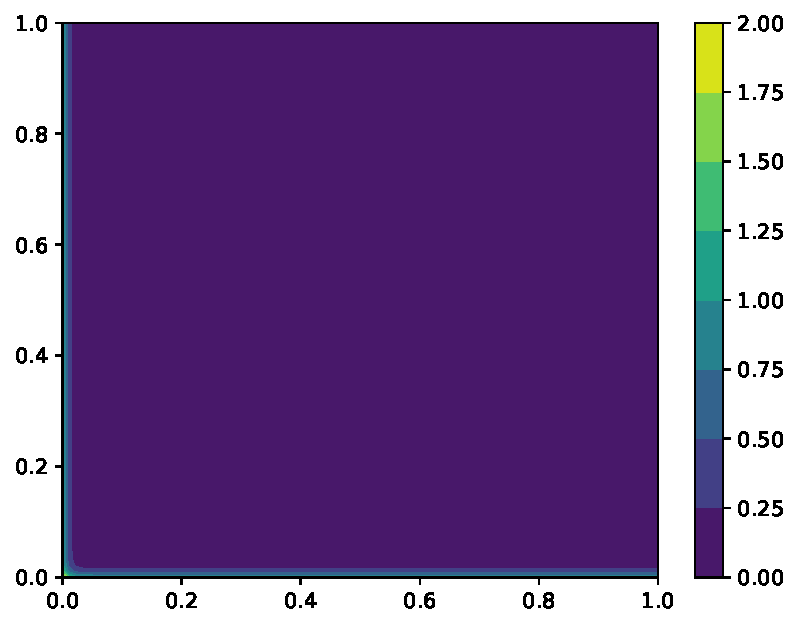
\includegraphics[width=0.32\linewidth]{ThesisFigs/bl2d_test.pdf}}
  \subfigure[\label{bl_2d_pred}SincKAN prediction]{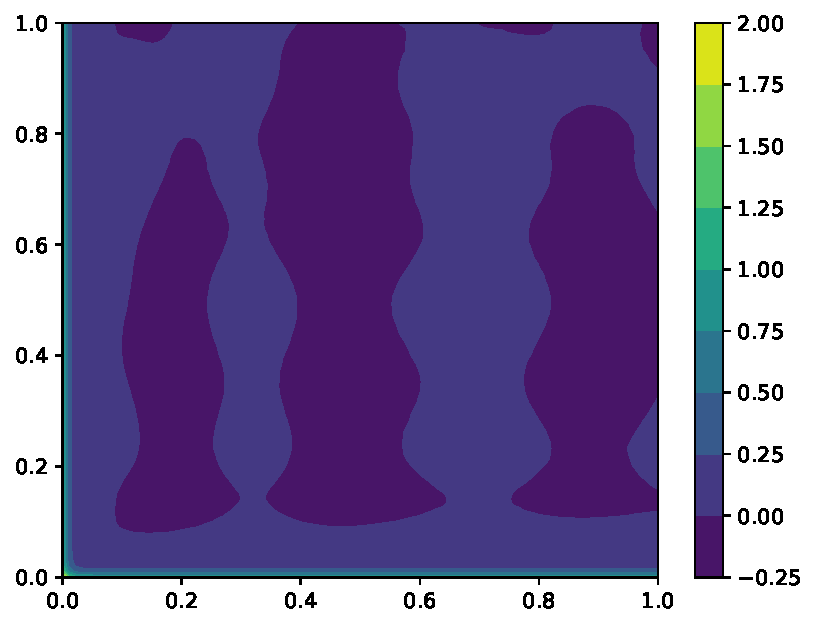
\includegraphics[width=0.32\linewidth]{ThesisFigs/bl2d_pred.pdf}}
  \subfigure[\label{bl_2d_error}Absolute error distribution]{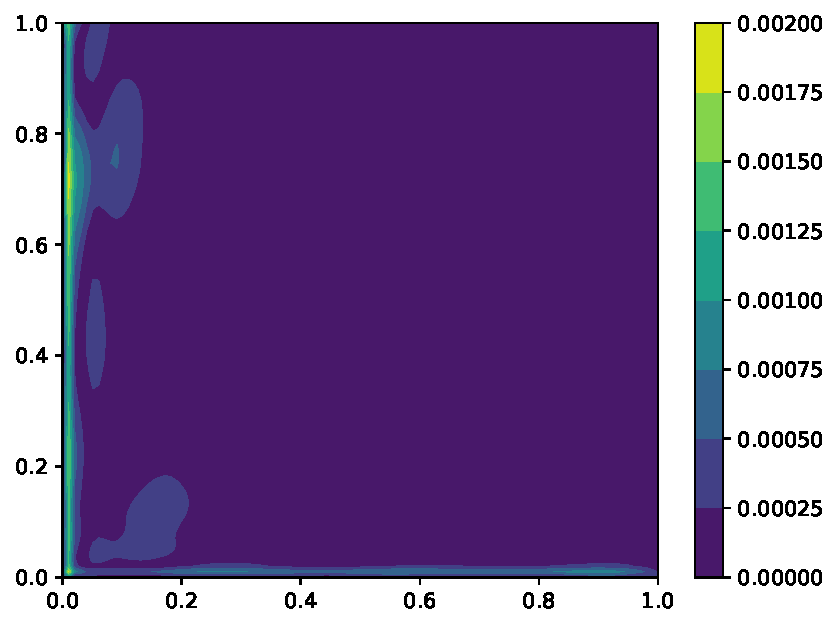
\includegraphics[width=0.32\linewidth]{ThesisFigs/bl2d_error.pdf}}
  \caption{Analysis of two-dimensional boundary layer problem: (a) exact solution of Equation~\ref{eq:bl2d}, (b) solution predicted by SincKAN, and (c) absolute error distribution, demonstrating that error concentrations primarily occur in the boundary layer region.}
  \label{fig:bl_2d}
\end{figure}

\subsubsection{Navier-Stokes Equations}
We examine the Taylor–Green vortex flow (components denoted as \textit{ns-tg-u} and \textit{ns-tg-v} in Table~\ref{table:pikan_pde}):
\begin{equation}
    \begin{gathered}
        \nabla \cdot \boldsymbol{u}=0, \quad t\in [0,T], \ \boldsymbol{x} \in \Omega,\\
        \partial_t \boldsymbol{u}+\boldsymbol{u} \cdot \nabla \boldsymbol{u}=-\nabla p+\nu\triangle \boldsymbol{u},\quad t\in [0,T], \ \boldsymbol{x} \in \Omega,
    \end{gathered}
\end{equation}
where $\boldsymbol{u}=(u,v)$. The system admits the exact solution:
\begin{equation}
    \begin{gathered}
        u = -\cos(x) \sin(y) \exp(-2\nu t), \\
        v = \sin(x) \cos(y) \exp(-2\nu t), \\
        p = -\left(\cos(2x) + \sin(2y)\right)\exp(-4\nu t)/4,
    \end{gathered}
\end{equation}
where $T=1$ and $\nu=1/400$. After non-dimensionalization, the spatial domain is $\boldsymbol{x} \in [0,1]^2$.

\section{Experimental Protocol}\label{Appendix: expeirment details}
All numerical experiments employ the Adam optimizer \citep{kingma2014adam} with exponential learning rate decay. The MLP and modified MLP architectures utilize hyperbolic tangent activation functions and Xavier initialization, following the methodology of \citet{raissi2019physics}.

\subsection{Function Approximation Protocol}
The hyperparameter configurations for the evaluated networks are presented in Table~\ref{table:cost for kans}. For one-dimensional problems, we implement the following protocol:

\begin{itemize}
    \item Training dataset generation: The input interval is uniformly discretized into 5000 points
    \item Training procedure: Each iteration randomly samples 3000 points from the training dataset
    \item Iteration count: Networks are trained for $10^5$ iterations
    \item Generalization assessment: Testing (fine) dataset comprises 10000 uniformly discretized points across the input interval
\end{itemize}

\subsection{PIKAN Implementation Protocol}
Network hyperparameters are specified in Table~\ref{table:cost for pikans}. The following protocols are implemented for different problem classes:

\begin{itemize}
    \item Time-independent one-dimensional problems:
    \begin{itemize}
        \item Training dataset: 1000 uniformly discretized points
        \item Sampling strategy: 500 random points per iteration
        \item Total iterations: $1.5 \times 10^6$
    \end{itemize}
    
    \item Time-dependent one-dimensional problems:
    \begin{itemize}
        \item Spatial discretization: 1000 points
        \item Temporal discretization: 11 points
        \item Sampling strategy: 5000 random points per iteration
        \item Total iterations: $1.5 \times 10^6$
    \end{itemize}
    
    \item Time-independent two-dimensional problems:
    \begin{itemize}
        \item Spatial discretization: 100 points per dimension
        \item Sampling strategy: 5000 random points per iteration
        \item Total iterations: $1.5 \times 10^6$
    \end{itemize}
    
    \item Time-dependent two-dimensional problems:
    \begin{itemize}
        \item Spatial discretization: 100 points per dimension
        \item Temporal discretization: 11 points
        \item Sampling strategy: 50000 random points per iteration
        \item Total iterations: $1.5 \times 10^6$
    \end{itemize}
    
    \item High-dimensional Poisson equation:
    \begin{itemize}
        \item Interior domain sampling: 2000 points per iteration
        \item Boundary domain sampling: 10000 points per iteration
        \item Test dataset composition: 8000 interior points and 2000 boundary points
        \item Total iterations: $5 \times 10^6$
    \end{itemize}
\end{itemize}

\subsection{Fractional PINN Implementation}\label{Appendix: fpinn}
Our implementation adopts the fPINNs framework \citep{pang2019fpinns}, utilizing the second-order Grünwald-Letnikov (GL) formula \citep{LISCHKE2020109009}:
\begin{equation}
(-\Delta)^{\alpha/2} u(x_j)=(1-\beta) \delta_{\Delta x, 1}^\alpha u(x_j)+\beta \delta_{\Delta x, 0}^\alpha u(x_j)+O((\Delta x)^2),
\end{equation}
where
\begin{equation}
\begin{aligned}
\delta_{\Delta x, p}^\alpha u(x_j) & :=(\Delta x)^{-\alpha} \sum_{k=0}^j(-1)^k\binom{\alpha}{k} u(x_j-(k-p) \Delta x)\\
& +(\Delta x)^{-\alpha} \sum_{k=0}^{N-j}(-1)^k\binom{\alpha}{k} u(x_j+(k-p) \Delta x).
\end{aligned}
\end{equation}

The computational domain $(0,1)$ is discretized with $\Delta x=1/N$, where $N=101$. We implement distinct learning rates: $10^{-2}$ for SincKAN and $10^{-3}$ for MLP. The networks are trained for $5\times10^5$ iterations, with SincKAN utilizing an architecture of $8\times 8 \times 1$. Performance metrics are presented in Figure~\ref{fig:frac_sol}.

\begin{figure}[ht]
  \centering
  \subfigure[$s=0.85$\label{sol_85}]{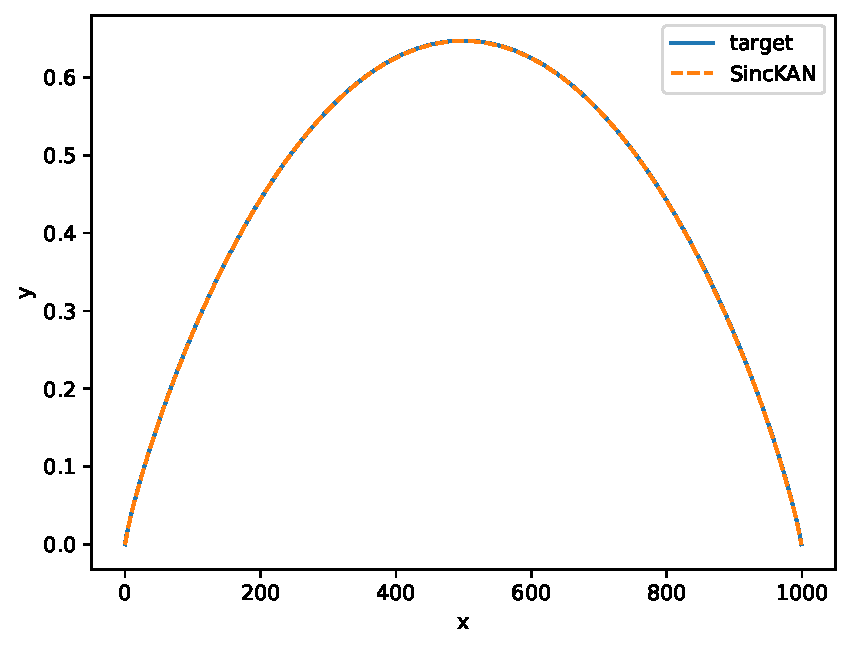
\includegraphics[width=0.32\linewidth]{ThesisFigs/frac_sol85.pdf}}
  \subfigure[$s=0.95$\label{sol_95}]{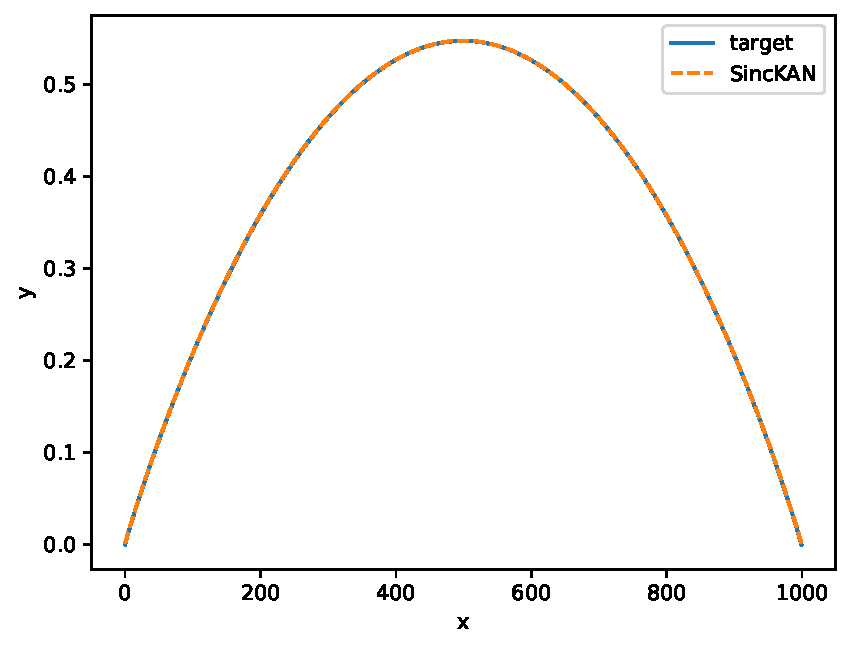
\includegraphics[width=0.32\linewidth]{ThesisFigs/frac_sol95.pdf}}
  \caption{Comparative analysis of target and SincKAN-predicted solutions for different fractional orders: (a) $s=0.85$ and (b) $s=0.95$.}
  \label{fig:frac_sol}
\end{figure}

\section{Analysis of SincKAN Interior Approximation}\label{Appendix: interior}
The internal approximation characteristics of SincKAN are demonstrated in Figure~\ref{fig:interior}.

\begin{figure}[ht]
   \centering
   \subfigure[\label{interior_approx}Equation~\ref{eq:bl2d} approximation analysis]{
\includegraphics[width=0.6\linewidth]{ThesisFigs/interior_approxi.pdf}}
   \subfigure[\label{interior_pde}PIKAN implementation analysis]{
\includegraphics[width=0.6\linewidth]{ThesisFigs/interior_pde.pdf}}
   \caption{Interior function analysis: (a) exhibits oscillatory behavior in interpolated $\phi$ due to high $M$ value implementation, while (b) demonstrates smoother $\phi$ characteristics resulting from low $M$ value implementation.}
   \label{fig:interior}
\end{figure}

\section{Generalization Analysis}\label{Appendix: fine grids}
As detailed in Section~\ref{Appendix: expeirment details}, we conduct additional evaluation on fine grid discretizations. Table~\ref{table: function fine grids} reveals certain limitations in SincKAN's generalization capabilities, suggesting areas for future research, although this limitation does not significantly impact the primary function approximation objectives.

\begin{table}[ht]
\caption{RMSE evaluated on fine grids}
\label{table: function fine grids}
\begin{center}
\begin{adjustbox}{width=\columnwidth, center}
\begin{tabular}{llllll}
\multicolumn{1}{c}{\bf Function name}  & \multicolumn{1}{c}{\bf MLP} & \multicolumn{1}{c}{\bf modified MLP} &\multicolumn{1}{c}{\bf KAN} & \multicolumn{1}{c}{\bf ChebyKAN} & \multicolumn{1}{c}{\bf SincKAN (ours)} 
\\ \hline 
\textit{sin-low} & $1.51 e\mbox{-}2 \pm 2.01 e\mbox{-}2$ & $7.29e\mbox{-}4 \pm 2.97 e\mbox{-}4$ & $1.27e\mbox{-}3 \pm 3.04e\mbox{-}4$ &
$1.76e\mbox{-}3 \pm 3.19e\mbox{-}4$ &
\textcolor{red}{$4.46 e\mbox{-}4 \pm 2.79 e\mbox{-}4$} \\ 
\textit{sin-high} & $7.07e\mbox{-}1 \pm 4.21e\mbox{-}8$ & $7.07 e\mbox{-}1 \pm 1.31 e\mbox{-}5$ & $7.06e\mbox{-}1 \pm 1.29e\mbox{-}3$ &
$5.70e\mbox{-}2 \pm 5.99 e\mbox{-}3$ &
\textcolor{red}{$4.15e\mbox{-}2 \pm 4.53e\mbox{-}3$} \\ 
\textit{bl} & $7.63e\mbox{-}4 \pm 1.13e\mbox{-}3$ & $5.72e\mbox{-}4 \pm 4.01e\mbox{-}4$ & $2.62e\mbox{-}4 \pm 7.89e\mbox{-}5$ &
$1.81e\mbox{-}3 \pm 6.98e\mbox{-}4$ &
\textcolor{red}{$2.28e\mbox{-}4 \pm 1.16e\mbox{-}4$} \\ 
\textit{double exponential} & $1.95e\mbox{-}3 \pm 8.17e\mbox{-}4$ & $7.76e\mbox{-}5 \pm 4.07e\mbox{-}5$ & $2.18e\mbox{-}4 \pm 1.51e\mbox{-}4$ &
$3.11e\mbox{-}3 \pm 2.16 e\mbox{-}3$ &
\textcolor{red}{$7.06e\mbox{-}5 \pm 1.09e\mbox{-}5$} \\ 
sqrt & $3.06e\mbox{-}3 \pm 9.34 e\mbox{-}4$ & \textcolor{red}{$4.46 e\mbox{-}5 \pm 5.51e\mbox{-}5$} & $4.79e\mbox{-}4 \pm 1.23e\mbox{-}4$ &
$3.69e\mbox{-}3 \pm 1.27 e\mbox{-}3$ &
$3.24e\mbox{-}4 \pm 1.31e\mbox{-}4$\\ 
\textit{multi-sqrt} & $2.06e\mbox{-}3 \pm 1.16e\mbox{-}3$ & $4.59e\mbox{-}4 \pm 4.86e\mbox{-}4$ & $3.61e\mbox{-}4 \pm 8.67 e\mbox{-}5$ &
$2.34e\mbox{-}3 \pm 1.17e\mbox{-}3$ &
\textcolor{red}{$2.14e\mbox{-}4 \pm 2.49 e\mbox{-}4$} \\ 
\textit{piece-wise} & $2.06e\mbox{-}2 \pm 5.57e\mbox{-}3$ & $3.75e\mbox{-}2 \pm 1.81e\mbox{-}2$ & $5.84e\mbox{-}2 \pm 1.03e\mbox{-}2$ &
\textcolor{red}{$7.28e\mbox{-}3 \pm 9.59 e\mbox{-}4$} &
$9.41e\mbox{-}3 \pm 2.14e\mbox{-}4$ \\ 
\textit{spectral-bias} & $2.48e\mbox{-}2 \pm 9.77 e\mbox{-}3$ & \textcolor{red}{$1.88e\mbox{-}2 \pm 9.55e\mbox{-}4$} & $4.79e\mbox{-}2 \pm 9.44 e\mbox{-}3$ &
$2.18e\mbox{-}2 \pm 2.97 e\mbox{-}4$ &
$2.21e\mbox{-}2 \pm 9.98 e\mbox{-}5$ \\ 
\end{tabular}
\end{adjustbox}
\end{center}
\end{table}

\section{Network Architecture Specifications}\label{Appendix: networks}
\subsection{Multilayer Perceptron}
The Multilayer Perceptron (MLP) architecture comprises fully connected neurons with nonlinear activation functions, expressed mathematically as:
\begin{equation}
\operatorname{MLP}(x)=\left(W^{L-1} \circ \sigma \circ W^{L-2} \circ \sigma \circ \cdots \circ W^1 \circ \sigma \circ W^0\right) \vx,
\end{equation}
where $W^i(x)=W_ix+b_i$, with $W_i \in \mathbb{R}^{m_i \times n_i}$ representing learnable matrices, $b_i \in \mathbb{R}^{m_i}$ denoting learnable bias terms, $\sigma$ representing the chosen nonlinear activation function, and $L$ indicating network depth.

\subsection{Modified MLP}
The Modified MLP architecture, inspired by transformer networks, incorporates two additional features with skip connections:
\begin{equation}
\begin{gathered}
    U=\sigma(W^{L+1}\vx), \quad V=\sigma(W^{L+2}\vx), \quad H^1=\sigma(W^{0}\vx), \\
    H^{i+1} = (1-\sigma(W^{i}H^{i}))*U+\sigma(W^{i}H^{i})*V, \quad i=1,\dots,L, \\
    \operatorname{Modified MLP}(\vx) = W^{L+3}H^{L+1},
\end{gathered}
\end{equation}
where $*$ denotes element-wise multiplication.

\subsection{Kolmogorov-Arnold Network}\label{Appendix: networks_kan}
\subsubsection{Theoretical Foundation}
The Kolmogorov-Arnold representation theorem establishes that any continuous multivariate function on a bounded domain can be represented through finite composition of univariate continuous functions and addition. Specifically, for a continuous function $f:[0,1]^n\rightarrow \mathbb{R}$, there exist continuous univariate functions $\phi_{q,p}$ and $\Phi_{q}$ such that:
\begin{equation}
    f(\mathbf{x})=f(x_1, \dots, x_n)=\sum_{q=1}^{2n+1} \Phi_q\left(\sum_{p=1}^n \phi_{q,p}(x_p)\right).
\end{equation}

\subsubsection{Architectural Implementation}
The Kolmogorov-Arnold Network (KAN) extends traditional neural architectures by implementing learnable activation functions. Let $\mathbf{\Phi}=\{\phi_{p,q}\}$ represent a matrix of univariate functions where $p= 1, 2, \dots n_{in}, q= 1, 2, \dots n_{out}$, and $\theta$ denote trainable parameters. The KAN is defined as:
\begin{equation}
    \operatorname{KAN} (\vx) = \left(\mathbf{\Phi}_{L-1} \circ \mathbf{\Phi}_{L-2} \circ \cdots \circ \mathbf{\Phi}_1 \circ \mathbf{\Phi}_0\right) \vx, \quad \vx\in \mathbb{R}^d,
\end{equation}
where:
\begin{equation}\label{eq: def phi}
\mathbf{\Phi}_{l}(\vx^{(l)})= \left\{\sum_{i=1}^{n^{(l)}_{in}} \phi_{j,i}(x_{i}^{(l)})\right\}_{j=1}^{n^{(l)}_{out}}, \quad \forall l = 0,1,\dots,L-1,
\end{equation}
with $\vx^{l} \in \mathbb{R}^{n_{in}^{(l)}}$ and $\mathbf{\Phi}_{l}(\vx^{(l)}) \in \mathbb{R}^{n_{out}^{(l)}}$. For a KAN of size $[n_0,n_1,\dots,n_L]$, we have $n^{(l)}_{in}=n_l$ and $n^{(l)}_{out}=n_{l+1}$.

Each activation function $\phi$ is approximated through a combination of basis functions and spline interpolation:
\begin{equation}
    \phi(x)=w_b \mathrm{silu}(x)+w_s \left(\sum_i^N c_i B_i(x)\right),
\end{equation}
where $c_i$, $w_s$, and $w_b$ are learnable parameters, $B_i$ represents the $k$-th order B-splines, $N=G+k-1$, and $G$ denotes the grid size.

\subsection{ChebyKAN Architecture}
The ChebyKAN architecture implements Chebyshev polynomials for the construction of learnable activation functions within the KAN framework. The modified ChebyKAN variant incorporates hyperbolic tangent activation functions between successive layers, yielding the following architectural formulation:
\begin{equation}
    \operatorname{ChebyKAN} (\vx) = \left(\mathbf{\Phi}_{L-1} \circ \tanh \circ \mathbf{\Phi}_{L-2}\circ \cdots \circ \mathbf{\Phi}_1 \circ \tanh \circ \mathbf{\Phi}_0\circ \tanh\right) \vx, \quad \vx\in \mathbb{R}^d,
\end{equation}
where $\mathbf{\Phi}$ maintains the definition from Equation~\ref{eq: def phi} with univariate functions:
\begin{equation}
    \phi = \sum_i c_i T_i(x),
\end{equation}
where $T_i$ represents the $i$-th Chebyshev polynomial.

\section{Computational Cost Analysis}\label{Appendix: cost}
\subsection{Training Complexity}
The SincKAN architecture, as defined in Equation~\ref{eq: Sinc activation function}, incorporates an additional summation over multiple step sizes $h$, resulting in trainable coefficients $c$ that are $M$ times larger than those in KAN and ChebyKAN implementations. However, total training time depends on multiple factors beyond parameter count. Tables~\ref{table:cost for kans} and \ref{table:cost for pikans} present comprehensive computational costs for approximation and PDE tasks, respectively.

In these tables, we employ the following notation conventions:
- MLP and modified MLP architectures: 'depth$\times$width'
- KAN and ChebyKAN architectures: 'width$\times$degree'
- SincKAN architecture: 'width$\times$degree$\times M

Network training was conducted in two distinct computational environments:
\begin{itemize}
    \item \dag: Single NVIDIA A100-SXM4-80GB GPU, CUDA version 12.4
    \item \ddag: Single NVIDIA A40-48GB GPU, CUDA version 12.4
\end{itemize}

\begin{table}[ht]
\caption{Computational Cost Analysis for Approximation Tasks\dag}
\label{table:cost for kans}
\begin{center}
\begin{tabular}{lllll}
\multicolumn{1}{c}{\textbf{Network}} & \multicolumn{1}{c}{\textbf{Architecture}} & \multicolumn{1}{c}{\textbf{Training Rate (iter/sec)}} & \multicolumn{1}{c}{\textbf{Reference Time (ms)}} & \multicolumn{1}{c}{\textbf{Parameters}} \\ \hline
MLP & $10\times 100$ & $9.89\times 10^2$ & $1.62\times 10^1$ & $81,101$ \\
Modified MLP & $10\times 100$ & $9.13\times 10^2$ & $2.92\times 10^1$ & $81,501$ \\
KAN & $8\times 8$ & $1.15\times 10^3$ & $1.01\times 10^2$ & $160$ \\
ChebyKAN & $40\times 40$ & $1.29\times 10^3$ & $3.11\times 10^1$ & $3,280$ \\
SincKAN & $8\times 100 \times 6$ & $1.29\times 10^3$ & $2.06\times 10^1$ & $9,696$ \\
\end{tabular}
\end{center}
\end{table}

\begin{table}[ht]
\caption{Computational cost for train PIKANs}
\label{table:cost for pikans}
\begin{center}
\begin{tabular}{lllll}
\multicolumn{1}{c}{\bf Function name}  & \multicolumn{1}{c}{\bf Network}& \multicolumn{1}{c}{\bf Size}  & \multicolumn{1}{c}{\bf Training rate (iter/sec)} & \multicolumn{1}{c}{\bf Parameters} \\ 
\hline 
\multirow{5}{*}{boundary layer$^\ddag$ } & MLP &$10\times 100$ & $6.47\times 10^{2}$ & 81101 \\
                      & modified MLP & $10\times 100$ &$3.55\times 10^{2}$ & 81501\\ 
                      & KAN & $8\times 8$  &$1.33\times 10^{3}$ & 160\\ 
                      & ChebyKAN & $40\times 40$ & $1.89\times 10^{3}$  & 3280\\ 
                      & SincKAN & $8\times 8 \times 1$ & $1.27\times 10^{3}$  & 194 \\ 
\\
\multirow{5}{*}{\textit{perturbed}$^\ddag$ } & MLP & $10\times 100$ & $6.85\times 10^{2}$ & 81101 \\ 
                      & modified MLP &$10\times 100$ & $3.59\times 10^{2}$ & 81501\\ 
                      & KAN & $8\times 8$ & $1.27\times 10^{3}$ & 160\\ 
                      & ChebyKAN & $40\times 40$ & $1.07\times 10^{3}$ & 3280 \\ 
                      & SincKAN & $8\times 8 \times 1$ & $1.25\times 10^{3}$ &194 \\ 
\\
\multirow{5}{*}{\textit{nonlinear}$^\ddag$ } & MLP & $10\times 100$ & $4.62\times 10^{2}$ & 81101\\ 
                      & modified MLP & $10\times 100$ & $3.07\times 10^{2}$ & 81501\\ 
                      & KAN & $8\times 8$ & $1.56\times 10^{3}$ & 160\\ 
                      & ChebyKAN & $40\times 40$ & $1.53\times 10^{3}$ & 3280 \\ 
                      & SincKAN & $8\times 4 \times 1$ & $1.54\times 10^{3}$ & 130 \\ 
\\
\multirow{5}{*}{\textit{bl-2d}$^\ddag$ } & MLP & $10\times 100$ & $2.39\times 10^{2}$ & 81201\\ 
                      & modified MLP & $10\times 100$ & $1.96\times 10^{2}$ & 81801\\ 
                      & KAN & $8\times 8$ & $3.46\times 10^{2}$ & 240\\ 
                      & ChebyKAN & $40\times 40$ & $4.95\times 10^{2}$ & 4920 \\ 
                      & SincKAN & $8\times 20 \times 1$ & $2.97\times 10^{2}$ & 570 \\ 
\\
\multirow{5}{*}{\textit{ns-tg}$^\dag$ } & MLP & $10\times 100$ & $1.71\times 10^{2}$ & 81503\\ 
                      & modified MLP & $10\times 100$ & $1.51\times 10^{2}$ & 82303\\ 
                      & KAN & $8\times 8$ & $2.55\times 10^{2}$ & 480\\ 
                      & ChebyKAN & $40\times 40$ & $3.83\times 10^{3}$ & 9840 \\ 
                      & SincKAN & $8\times 8 \times 1$ & $2.77\times 10^{2}$ & 550 \\ 
\end{tabular}
\end{center}
\end{table}

\subsection{Reference Time Analysis}
The computational cost of reference operations exhibits independence from the specific task formulation (i.e., the loss function). Results evaluated on models trained for approximation tasks are presented in Table~\ref{table:cost for kans}. Despite SincKAN's larger parameter count compared to KAN and ChebyKAN, it demonstrates superior reference operation efficiency. This performance advantage is attributable to the compilation of training procedures using JAX~\cite{jax2018github}, which optimizes computational operations.

\section{Degree-Data Size Relationship Analysis}\label{Appendix: scaling law}
In traditional Sinc numerical methods, the number of sampled points equals the degree ($N_{degree}=N_{points}$), as each degree requires a corresponding function value $f(jh)$ at point $jh$. However, this equivalence proves impractical and unnecessary in the SincKAN framework, where multi-layer representation provides exponentially increasing capacity with depth \citep{yarotsky2017error}. To investigate the relationship between degree and data size, we conducted a comprehensive empirical analysis of SincKAN performance under varying $N_{degree}$ and $N_{points}$ configurations.

The experimental protocol employed the \textit{spectral-bias} function with the following parameter space:
\begin{itemize}
    \item Degrees: $N \in \{8,16,32,64,100,300\}$
    \item Data points: $N_{points} \in \{100,500,1000,5000,10000\}$
    \item Batch size adaptation: $N_{batch}=N_{points}/4$
\end{itemize}

Additional parameters were fixed at:
\begin{itemize}
    \item Inverse decay sequence: $\{h_i\}_{i=1}^M$ with $M=6$
    \item Base step size: $h_0=7.0$
\end{itemize}

Results are presented in Table~\ref{table: degree_points} and visualized in Figure~\ref{fig:degree_points}. Of particular note, Figure~\ref{degree_100} demonstrates that our neural scaling follows $\mathrm{RMSE} \propto G^{-4}$, surpassing the best scaling law $\mathrm{RMSE} \propto G^{-3}$ reported in KAN~\citep{liu2024kan}.
\begin{table}[ht]
\caption{RMSE for different degree and $N_{points}$}
\label{table: degree_points}
\begin{center}
\begin{adjustbox}{width=\columnwidth, center}
\begin{tabular}{clllll}
degree $\setminus$ $N_{points}$& \multicolumn{1}{c}{100} &\multicolumn{1}{c}{500} & \multicolumn{1}{c}{1,000} & \multicolumn{1}{c}{5,000} & \multicolumn{1}{c}{10,000}
\\ \hline
8 &$2.60e\mbox{-}1 \pm 2.76e\mbox{-}5$     & $1.16e\mbox{-}1 \pm 6.34e\mbox{-}6$   & $8.23e\mbox{-}2 \pm 4.54e\mbox{-}6$ & $6.70e\mbox{-}2 \pm 3.91e\mbox{-}3$ & $6.81e\mbox{-}2 \pm 4.51e\mbox{-}3$ \\
16                         & $1.01e\mbox{-}2 \pm 1.47e\mbox{-}2$  & $1.30e\mbox{-}3 \pm 9.42e\mbox{-}4$   & $1.04e\mbox{-}3 \pm 3.74e\mbox{-}4$ & $1.62e\mbox{-}3 \pm 2.48e\mbox{-}4$ & $9.57e\mbox{-}4 \pm 4.35e\mbox{-}4$ \\
32                         & \textcolor{red}{$3.63e\mbox{-}5 \pm 5.79e\mbox{-}5$}   & $2.69e\mbox{-}4 \pm 2.27e\mbox{-}4$   & $4.72e\mbox{-}4 \pm 2.75e\mbox{-}4$ & $2.15e\mbox{-}3 \pm 1.57e\mbox{-}3$ & $3.08e\mbox{-}3 \pm 7.14e\mbox{-}4$ \\
  64                       & $1.29e\mbox{-}3 \pm 2.21e\mbox{-}3$  & $5.60e\mbox{-}4 \pm 6.42e\mbox{-}4$   & $2.74e\mbox{-}3 \pm 4.01e\mbox{-}3$ & $1.83e\mbox{-}3 \pm 8.49e\mbox{-}4$ & $2.13e\mbox{-}3 \pm 9.05e\mbox{-}4$ \\
100 &$7.66e\mbox{-}5 \pm 1.16e\mbox{-}4$    & $3.79e\mbox{-}4 \pm 6.27e\mbox{-}4$  & $4.24e\mbox{-}4 \pm 7.42e\mbox{-}5$ & $2.19e\mbox{-}3 \pm 1.62e\mbox{-}3$ & $2.64e\mbox{-}3 \pm 1.76e\mbox{-}3$  \\ 
 300                        & $3.73e\mbox{-}4 \pm 5.62e\mbox{-}4$  &  $7.30e\mbox{-}5 \pm 4.25e\mbox{-}5$ & $7.54e\mbox{-}4 \pm 8.73e\mbox{-}4$ & $2.21e\mbox{-}3 \pm 1.04e\mbox{-}3$ & $2.18e\mbox{-}3 \pm 1.12e\mbox{-}3$  \\ 
\end{tabular}
\end{adjustbox}
\end{center}
\end{table}

\begin{figure}[ht]
  \centering
  \subfigure[\label{degree_100}$N_{points}=100$]{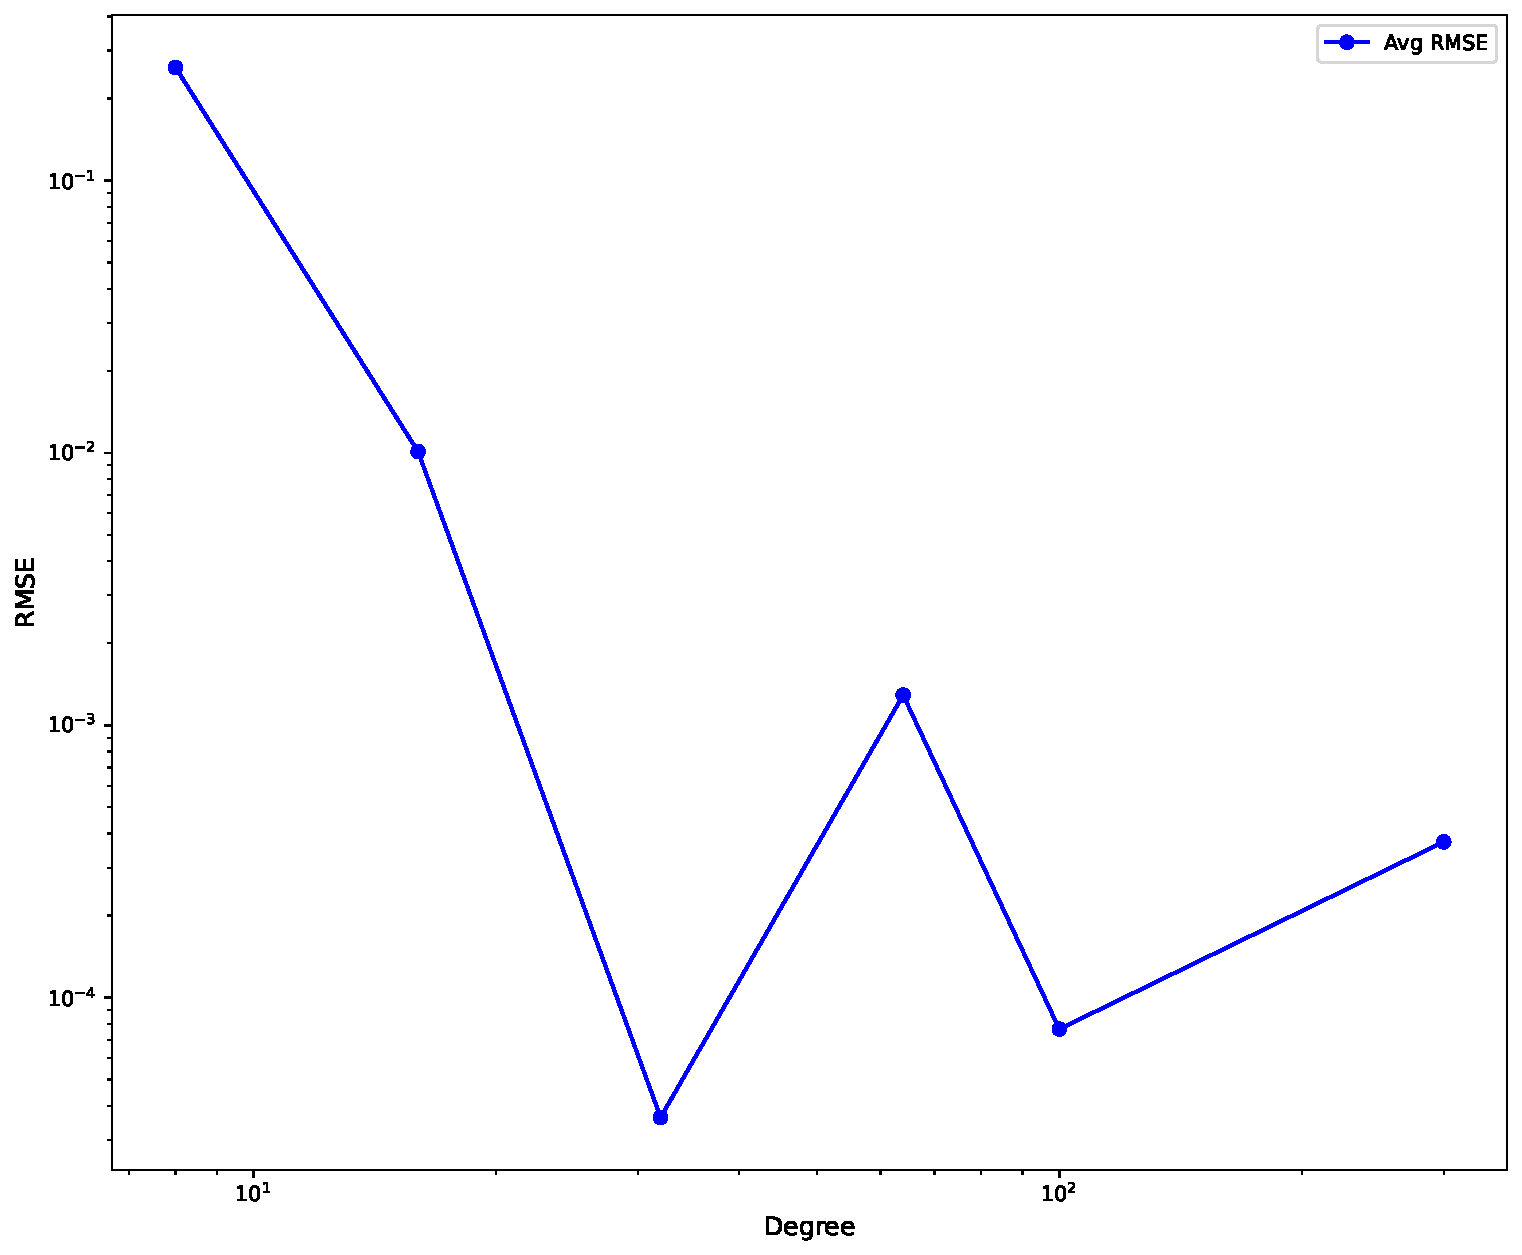
\includegraphics[width=0.3\linewidth]{ThesisFigs/degree_npoint_100.pdf}}
  \subfigure[\label{degree_500}$N_{points}=500$]{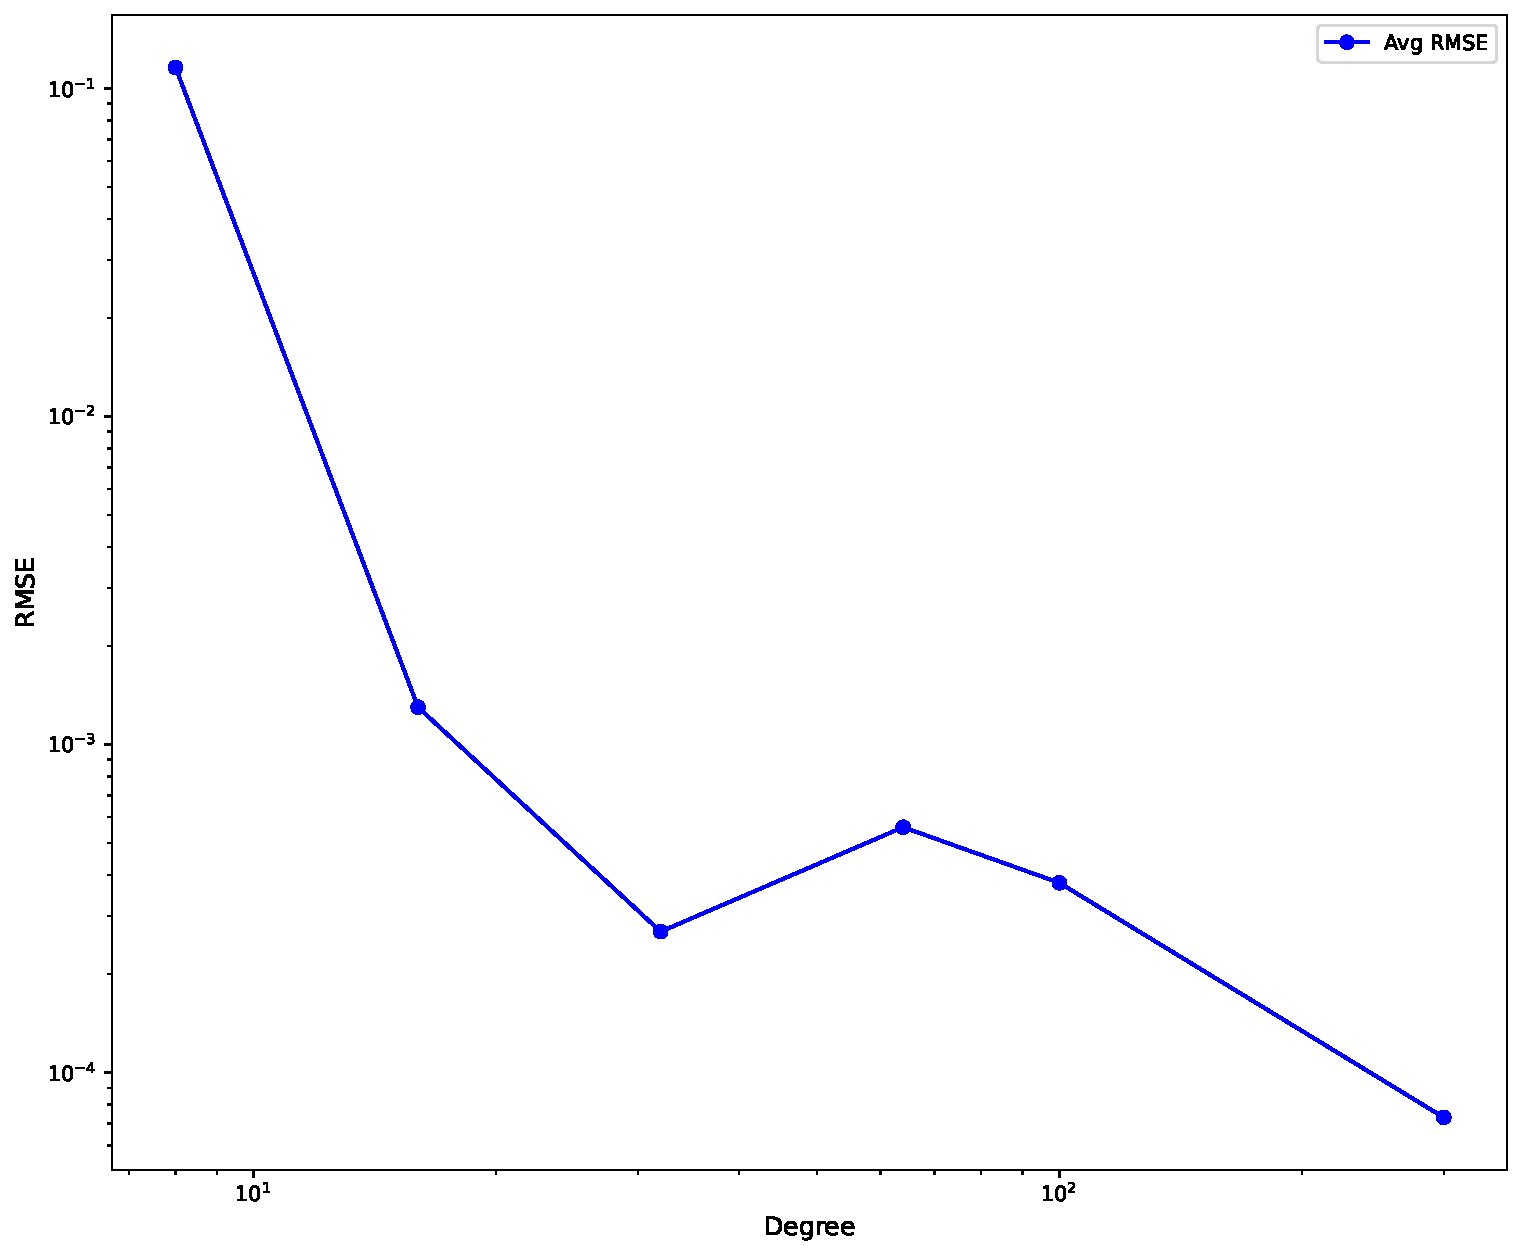
\includegraphics[width=0.3\linewidth]{ThesisFigs/degree_npoint_500.pdf}}
  \subfigure[\label{degree_1000}$N_{points}=1000$]{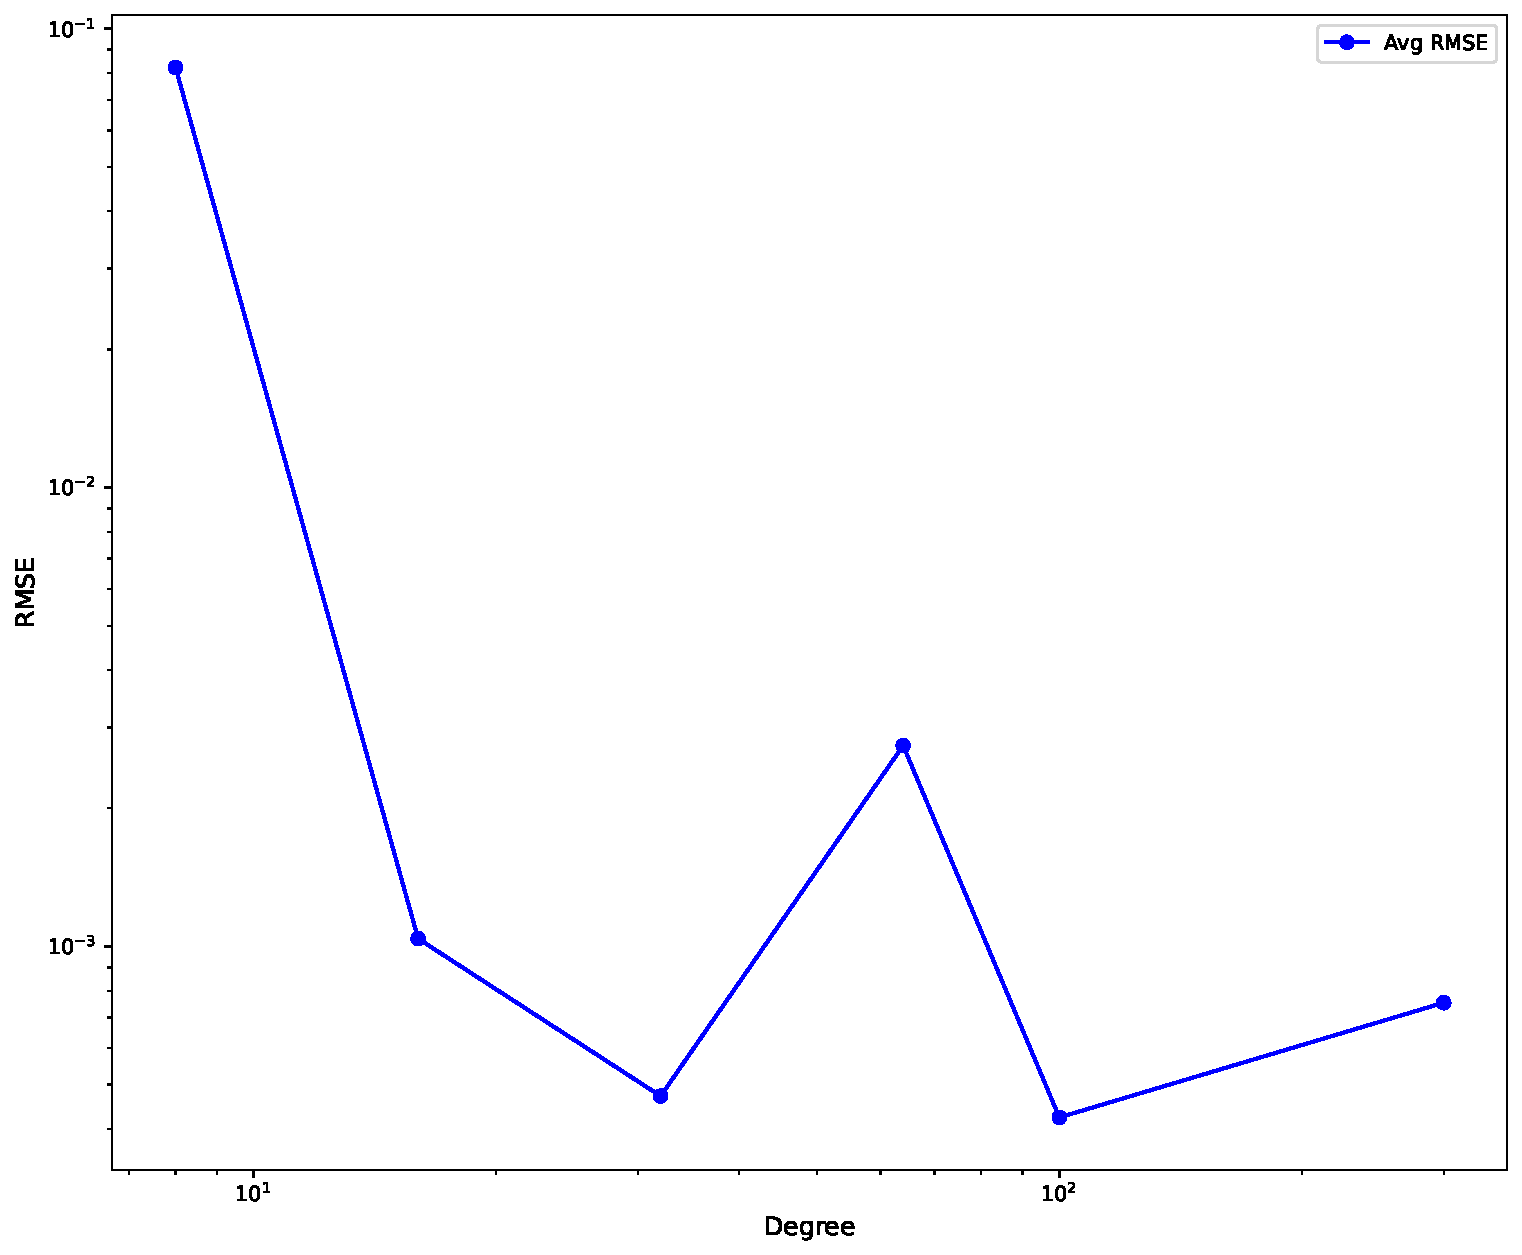
\includegraphics[width=0.3\linewidth]{ThesisFigs/degree_npoint_1000.pdf}}
  \subfigure[\label{degree_5000}$N_{points}=5000$]{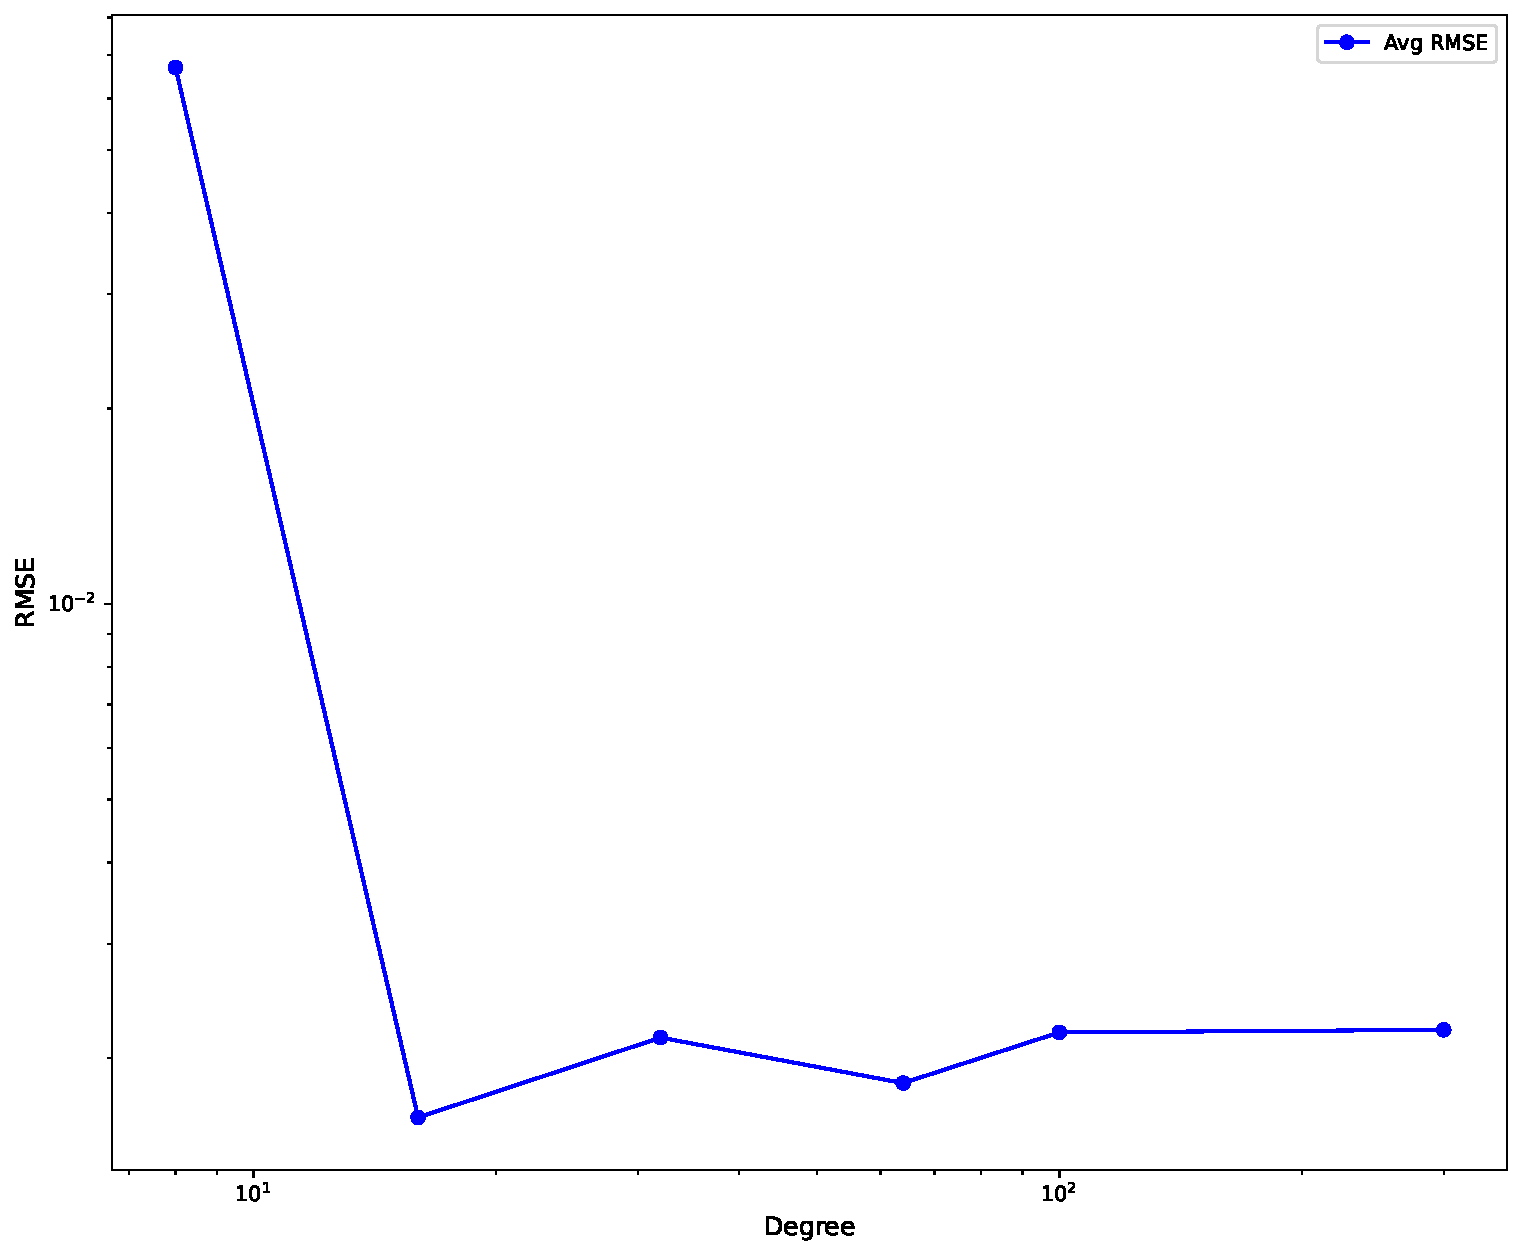
\includegraphics[width=0.3\linewidth]{ThesisFigs/degree_npoint_5000.pdf}}
  \subfigure[\label{degree_10000}$N_{points}=10000$]{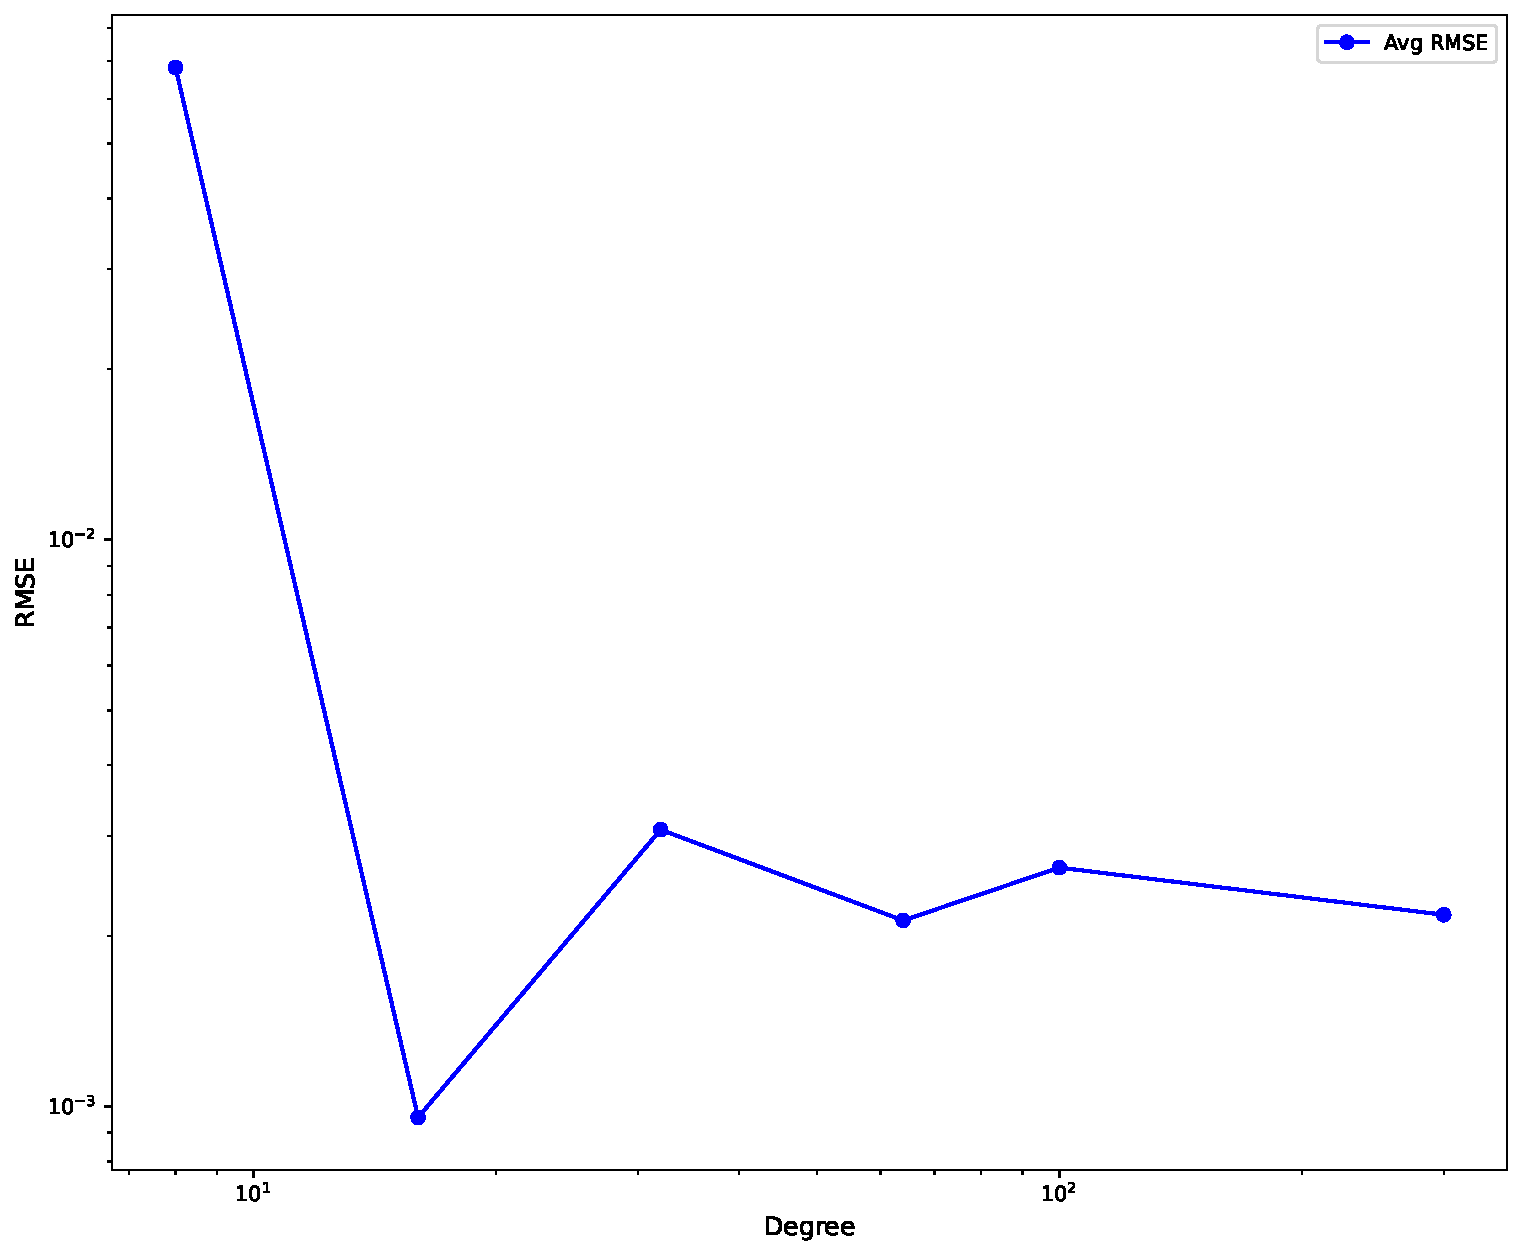
\includegraphics[width=0.3\linewidth]{ThesisFigs/degree_npoint_10000.pdf}}
  \caption{Performance analysis across varying $N_{points}$ configurations with increasing degree specifications.}
  \label{fig:degree_points}
\end{figure}

\section{Basis Update Strategy}\label{Appendix: update}
The interpolation methodology for each $\phi$ component represents a critical element of KAN architectures. However, the optimal degree for interpolation methods typically requires empirical determination. Table~\ref{table: degree_points} demonstrates that increased degree does not necessarily correlate with improved accuracy, potentially due to over-parameterization effects. To address this limitation, we propose Algorithm~\ref{algorithm: grids} for grid extension, enabling SincKAN to progress from small to large degrees adaptively.

\begin{algorithm}[ht]
   \caption{Grid Extension Protocol}
   \label{algorithm: grids}
   \begin{algorithmic}[1] 
       \Require $M > N > 0, \{c_i\}_{i=-N}^{N}$
       \Ensure $\{c^\prime_i\}_{i=-M}^{M}$
       \For{$i = -M$ \textbf{to} $M$}
           \If{$i \in [-N, N]$}
               \State $c_i^\prime \gets c_i$
           \Else
               \State $c_i^\prime \gets 0$
           \EndIf
       \EndFor
   \end{algorithmic}
\end{algorithm}
This methodology was evaluated using identical hyperparameters as described in \cref{Appendix: scaling law}, specifically focusing on \textit{spectral-basis} and \textit{bl} functions. In the initial experiment, a constant degree of $N_{degree}=100$ was established. For the variable degree implementation, the initialization began at $N_{degree}=8$, with subsequent updates following the sequence $\left[8, 8, 8, 8, 8, 8, 8, 8, 8, 8, 4, 4, 4\right]$ over 13 iterations until reaching $N_{degree}=100$. The constant degree model underwent training for $1.4\times 10^6$ iterations. In the variable degree configuration, each degree was trained for $10^5$ iterations, maintaining a cumulative training duration of $1.4\times10^6$ iterations, with the resultant grid updates illustrated in \cref{fig:update}. Upon observation of potential overfitting at $N_{degree}=100$, a second experiment was conducted with a reduced constant degree of $N_{degree}=96$. The variable degree implementation in this case commenced at $N_{degree}=8$, with progressive updates of $\left[8, 8, 8, 8, 8, 8, 8, 8, 8, 8, 4, 4\right]$ over 13 iterations until achieving $N_{degree}=96$. The constant degree model underwent training for $1.3\times 10^6$ iterations, while the variable degree configuration maintained $10^5$ iterations per degree, resulting in an equivalent total of $1.3\times10^6$ iterations. The corresponding grid updates are presented in \cref{fig:update_96}.
It is noteworthy that the computational efficiency of the variable degree approach marginally exceeds that of the constant degree method, owing to the optimization of basis changes. The comparative computational costs are detailed in \cref{table:cost for update}.
\begin{figure}[ht]%[H]%
\centering %%$u_t = \epsilon{\partial^6 u\over \partial x^6}$ %%$u_t = \epsilon{\partial^{10} u\over \partial x^{10}}$
\subfigure[\textit{bl}\label{update_bl_no}]{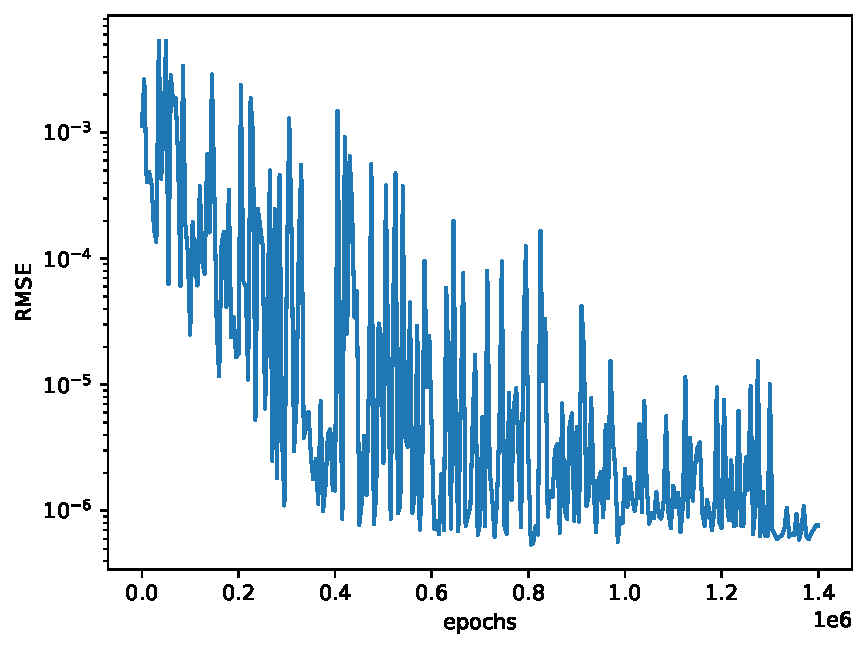
\includegraphics[width=0.42\linewidth]{ThesisFigs/bl_RMSE_001.pdf}}
\subfigure[\textit{bl}\label{update_bl_noinit}]{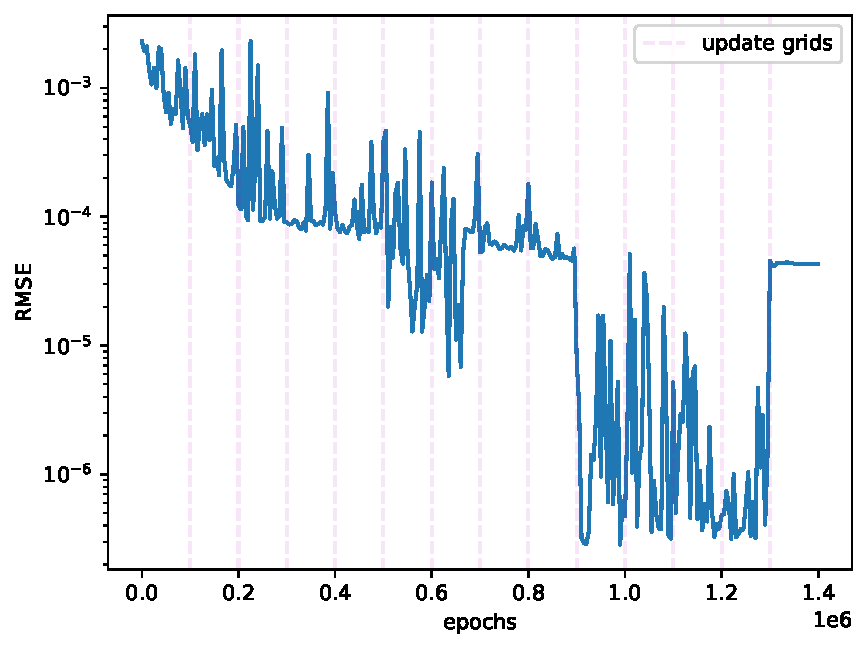
\includegraphics[width=0.42\linewidth]{ThesisFigs/bl_RMSE_010.pdf}}
\subfigure[\textit{spectral-basis}\label{update_sb_no}]{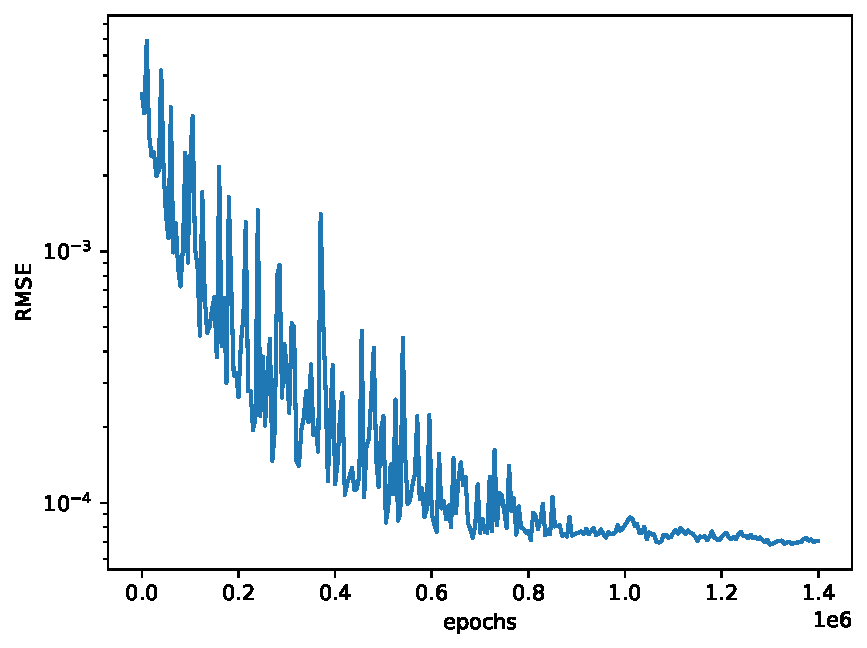
\includegraphics[width=0.42\linewidth]{ThesisFigs/sb_RMSE_001.pdf}}
\subfigure[\textit{spectral-basis}\label{update_sb_noinit}]{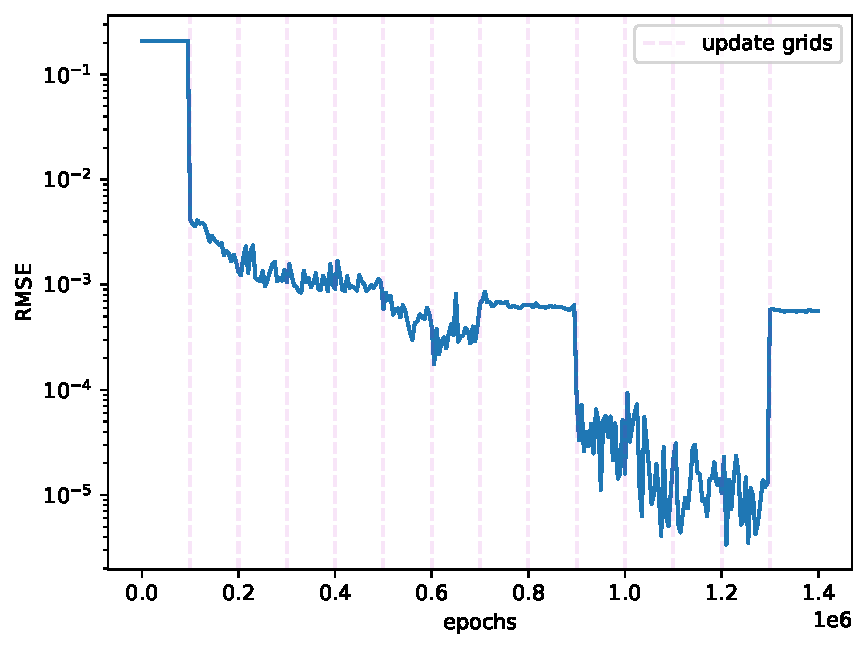
\includegraphics[width=0.42\linewidth]{ThesisFigs/sb_RMSE_010.pdf}}
\caption{For \textit{bl} and \textit{spectral-basis}, \cref{update_bl_no} and \cref{update_sb_no} correspondingly shows the RMSE for the constant degree $N_{degree}=100$; \cref{update_bl_noinit} and \cref{update_sb_noinit} correspondingly shows the RMSE for the variable degree}
\label{fig:update}
\end{figure}
\begin{figure}[ht]%[H]%
\centering %%$u_t = \epsilon{\partial^6 u\over \partial x^6}$ %%$u_t = \epsilon{\partial^{10} u\over \partial x^{10}}$
\subfigure[\textit{bl}\label{update_bl_no96}]{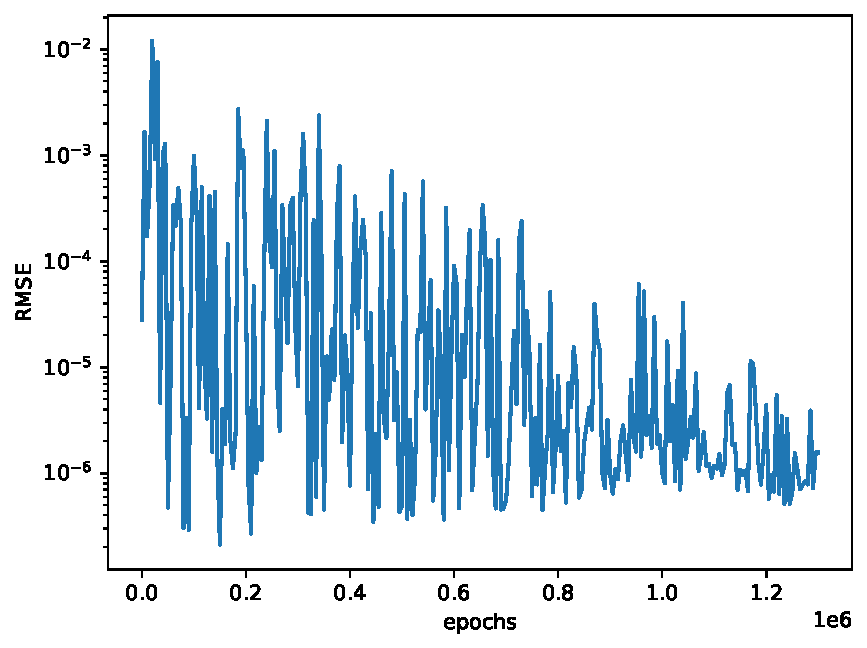
\includegraphics[width=0.42\linewidth]{ThesisFigs/bl_RMSE_001_96.pdf}}
\subfigure[\textit{bl}\label{update_bl_noinit96}]{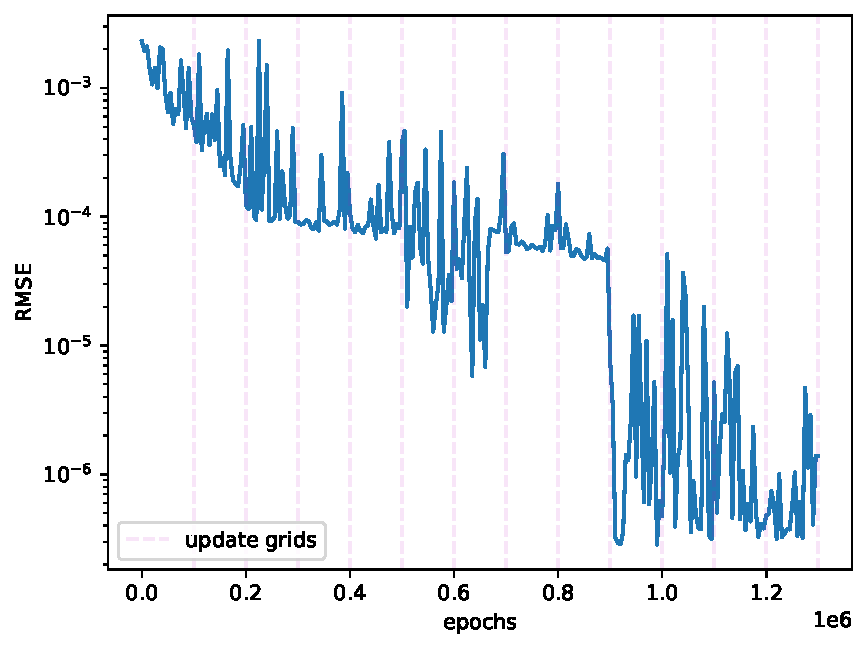
\includegraphics[width=0.42\linewidth]{ThesisFigs/bl_RMSE_010_96.pdf}}
\subfigure[\textit{spectral-basis}\label{update_sb_no96}]{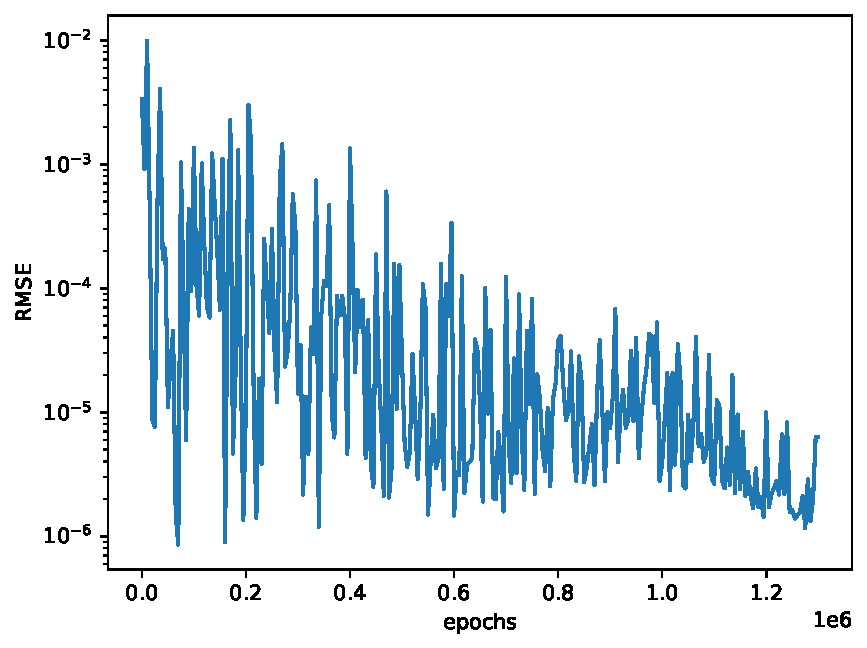
\includegraphics[width=0.42\linewidth]{ThesisFigs/sb_RMSE_001_96.pdf}}
\subfigure[\textit{spectral-basis}\label{update_sb_noinit96}]{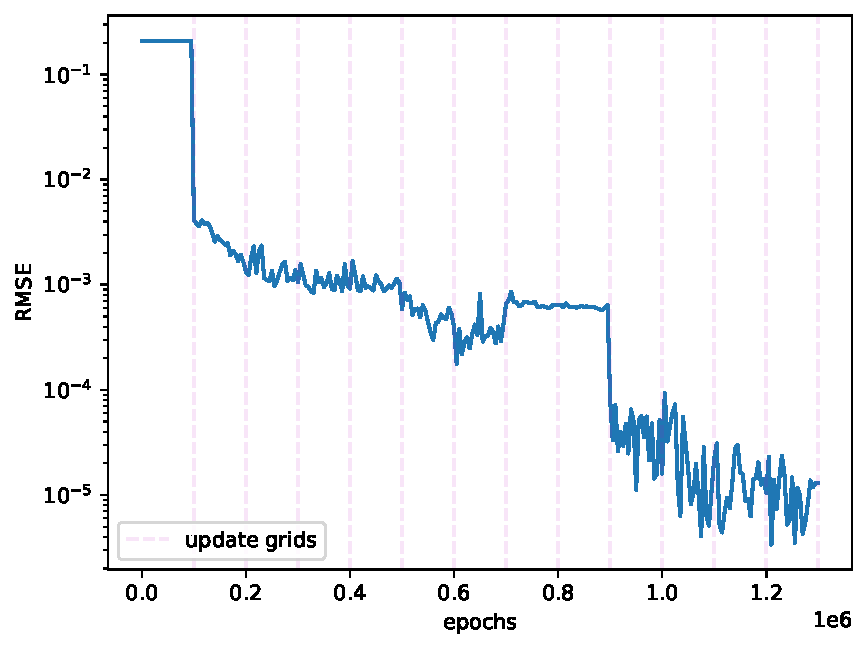
\includegraphics[width=0.42\linewidth]{ThesisFigs/sb_RMSE_010_96.pdf}}
\caption{For \textit{bl} and \textit{spectral-basis}, \cref{update_bl_no96} and \cref{update_sb_no96} correspondingly shows the RMSE for the constant degree $N_{degree}=96$; \cref{update_bl_noinit96} and \cref{update_sb_noinit96} correspondingly shows the RMSE for the variable degree}
\label{fig:update_96}
\end{figure}

\begin{table}[ht]
\caption{Computational cost for update of grids}
\label{table:cost for update}
\begin{center}
\begin{tabular}{lll}
% \multicolumn{1}{c}{\bf Type}  & \multicolumn{1}{c}{\bf Function}  & \multicolumn{1}{c}{\bf Training rate (iter/sec)} \\ 
\hline
constant degree & \textit{spectral-bias} & $7.82\times 10^2$ \\
variable degree & \textit{spectral-bias} & $7.82\times 10^2$ \\
constant degree & \textit{bl} & $7.67\times 10^2$ \\
variable degree & \textit{bl} & $7.73\times 10^2$ \\
\end{tabular}
\end{center}
\end{table}

\section{Results of selected $h$}\label{Appendix: select_h}
The comprehensive results of the selected ${h_i}$ parameters are presented in \cref{table: sin-low with inverse decay} and \cref{table: sin-low with exponential decay}. The complexity of parameter optimization increases substantially when $h_i$ assumes larger values. For instance, regarding large $h$ values on fine grids, it is hypothesized that $N_{degree}=100$ may not fully exploit the available capabilities. Consequently, an additional experimental investigation was conducted utilizing 5000 grid points, with ${h_i}={1/10,1/100,1/1000}$, and $N_{degree}=500$. The results demonstrated RMSE values of $7.92e\mbox{-}4\pm 4.21e\mbox{-}4$ for sin-low and $2.32e\mbox{-}3\pm 2.74e\mbox{-}4$ for sin-high. These findings indicate that enhanced accuracy can be achieved for sin-high through further hyperparameter optimization of the SincKAN model.
\begin{figure}[ht]%[H]%
\centering %%$u_t = \epsilon{\partial^6 u\over \partial x^6}$ %%$u_t = \epsilon{\partial^{10} u\over \partial x^{10}}$
\subfigure[\label{sin_low_inverse}]{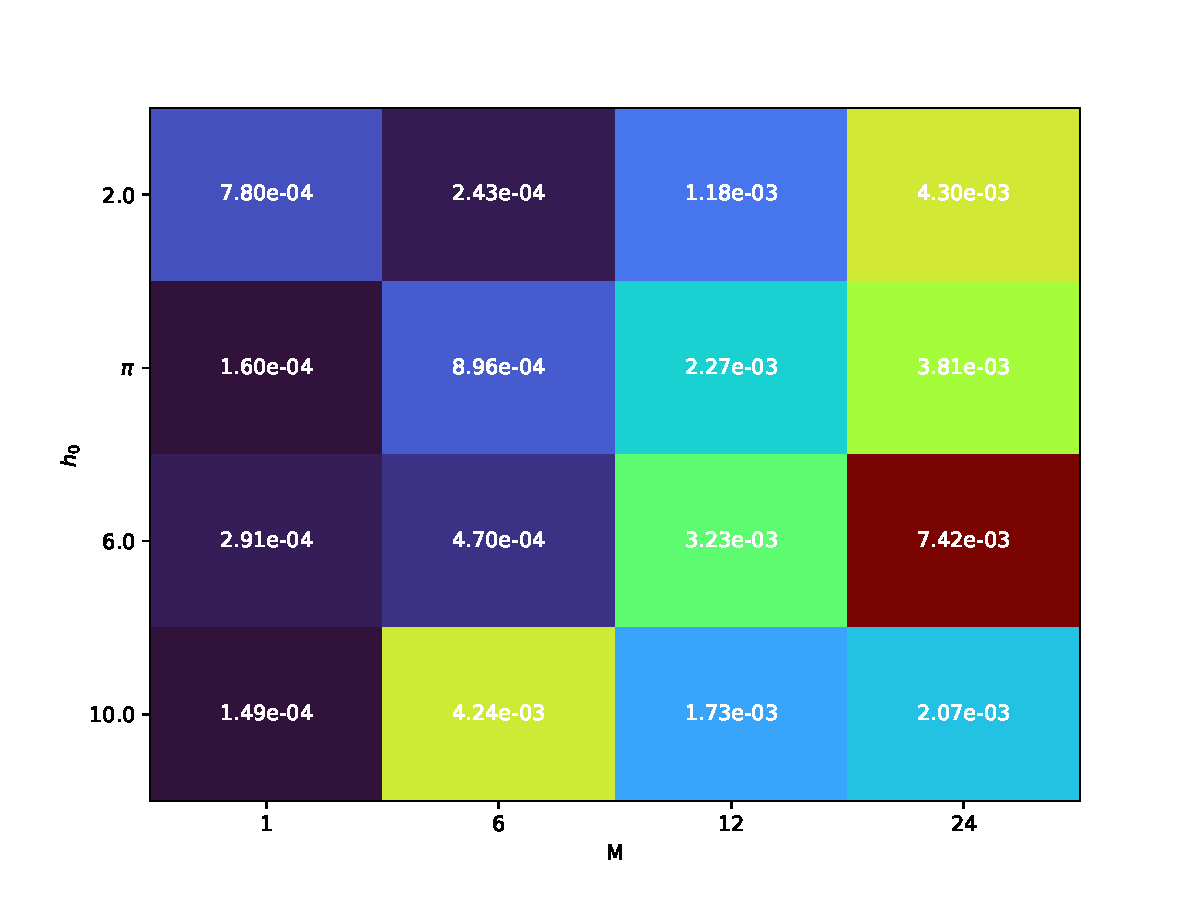
\includegraphics[width=0.4\linewidth]{ThesisFigs/sin_low_inverse.pdf}} %width==0.329
\subfigure[\label{sin_high_inverse}]{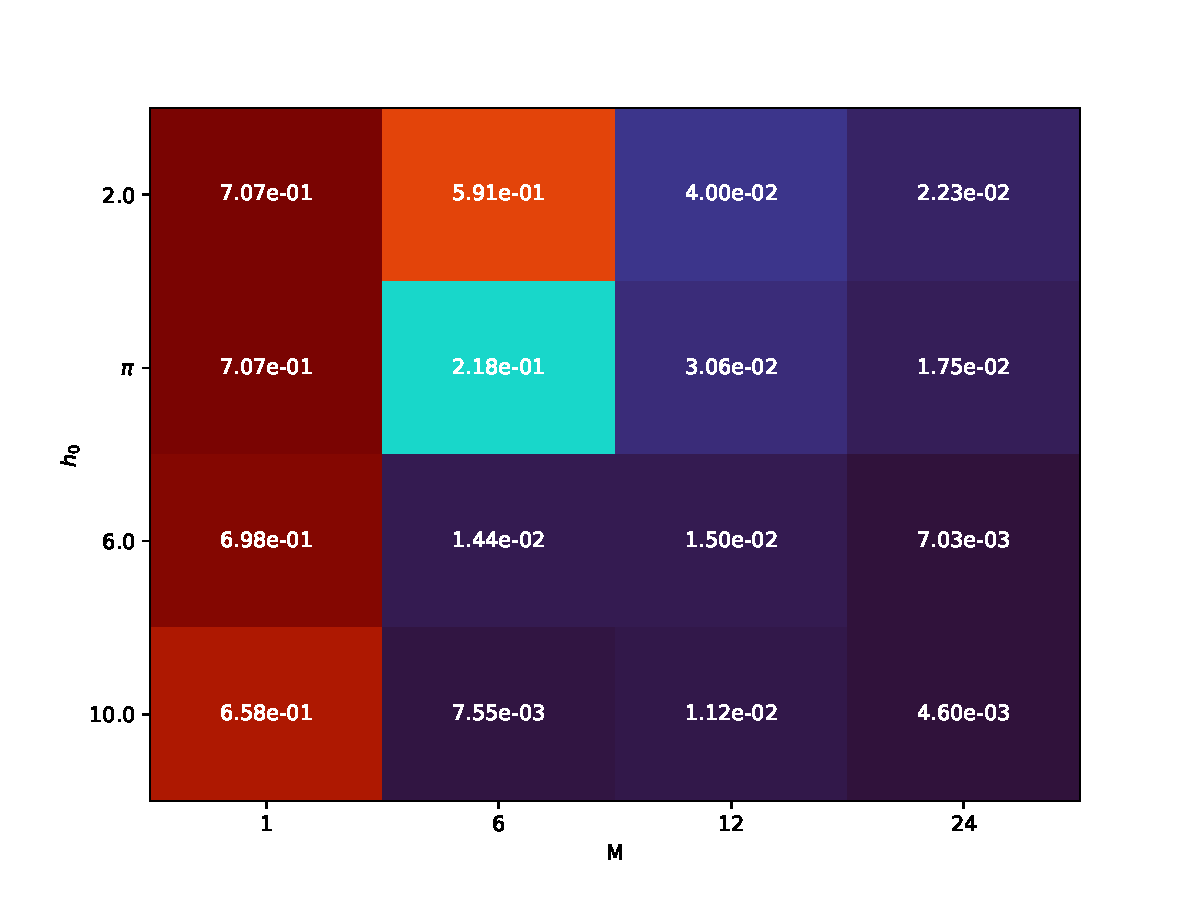
\includegraphics[width=0.4\linewidth]{ThesisFigs/sin_high_inverse.pdf}}
\caption{\cref{sin_low_inverse} shows the inverse decay approach on sin-low function; \cref{sin_high_inverse} shows the inverse decay approach on sin-high function.}
\label{fig:select_h_inverse}
\end{figure}
\begin{figure}[ht]%[H]%
\centering %%$u_t = \epsilon{\partial^6 u\over \partial x^6}$ %%$u_t = \epsilon{\partial^{10} u\over \partial x^{10}}$
\subfigure[\label{sin_low_exp}]{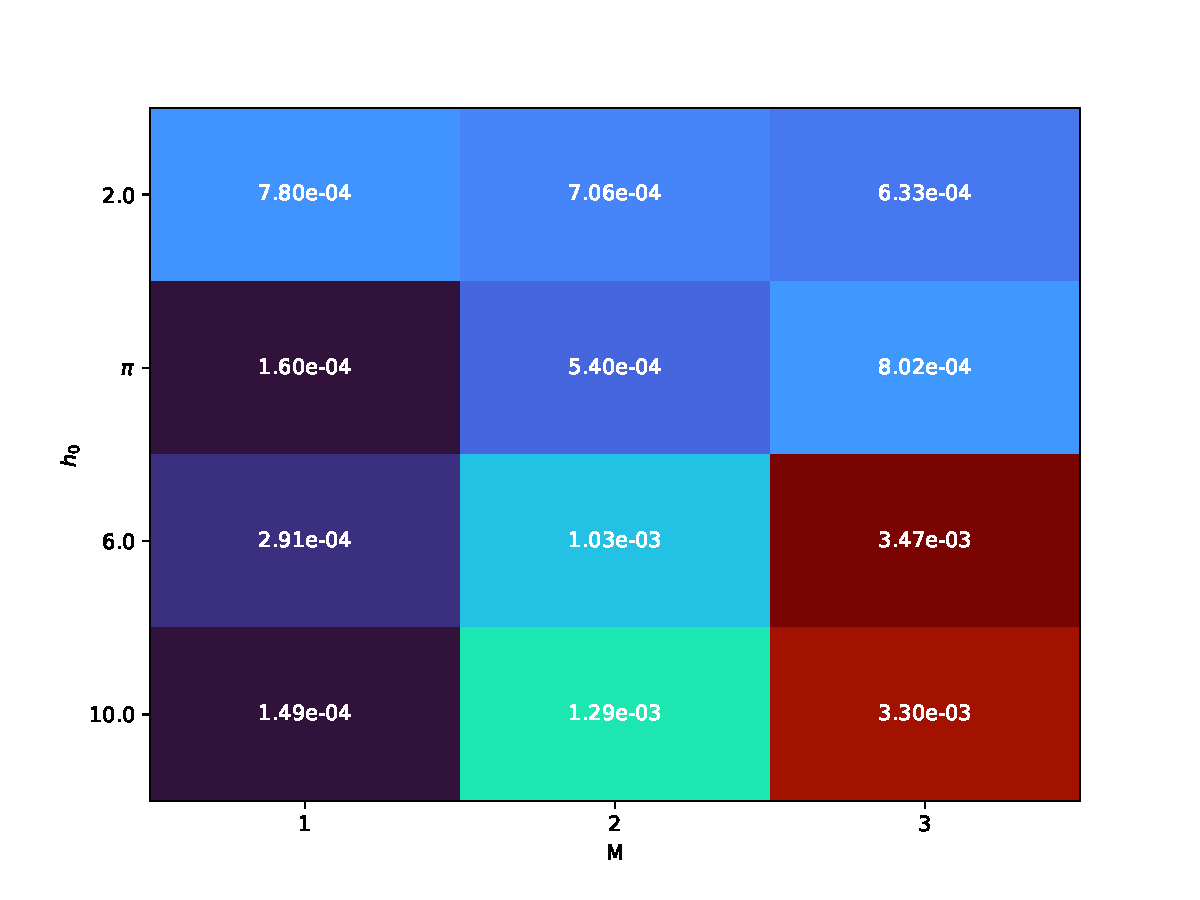
\includegraphics[width=0.4\linewidth]{ThesisFigs/sin_low_exp.pdf}}
\subfigure[\label{sin_high_exp}]{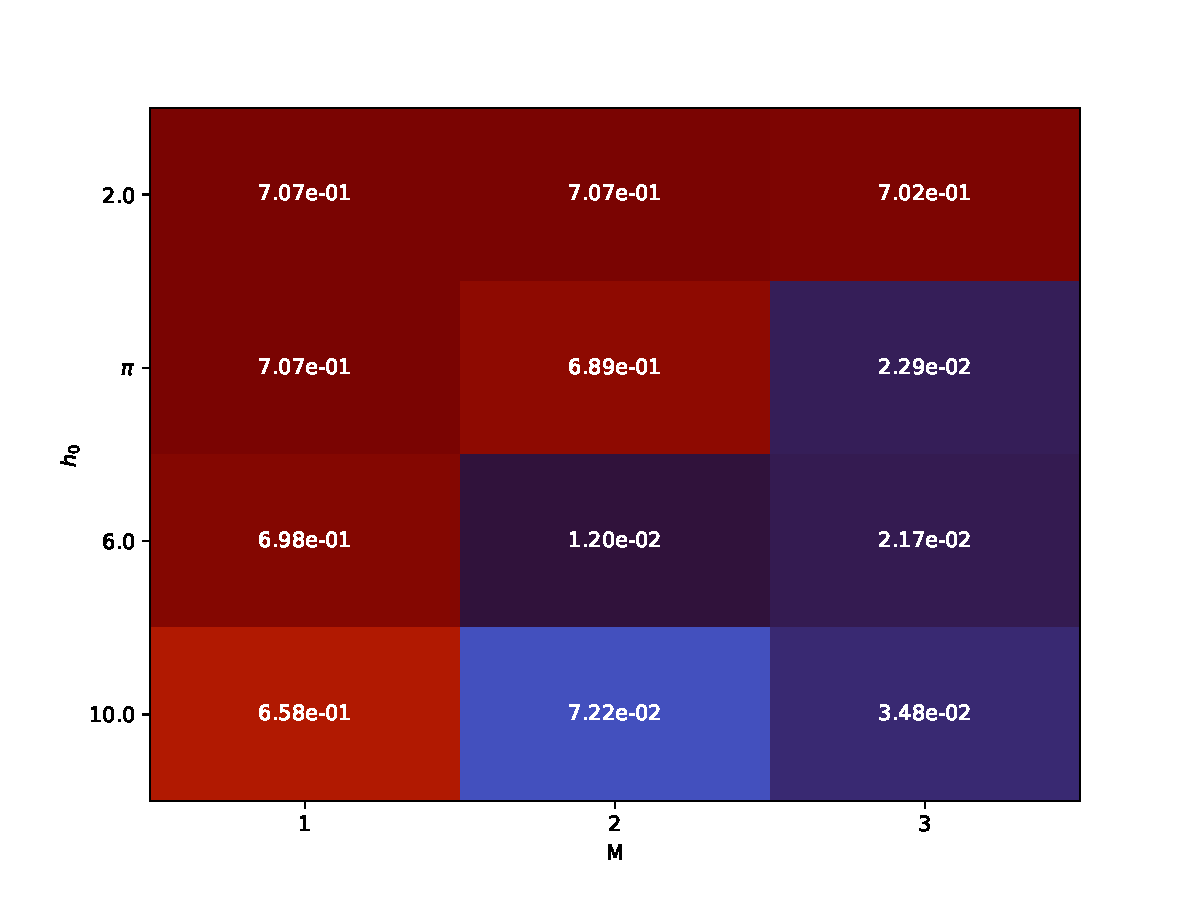
\includegraphics[width=0.4\linewidth]{ThesisFigs/sin_high_exp.pdf}}
\caption{\cref{sin_low_exp} shows the exponential decay approach on sin-low function; \cref{sin_high_exp} shows the exponential decay approach on sin-high function.}
\label{fig:select_h_exp}
\end{figure}
\begin{table}[ht]
\caption{RMSE for different $\{h_i\}$ with inverse decay}
\label{table: sin-low with inverse decay}
\begin{center}
\begin{adjustbox}{width=\columnwidth, center}
\begin{tabular}{llllll}
\multicolumn{1}{c}{\bf Function name}&$h_0$ $\setminus$ M& \multicolumn{1}{c}{1} &\multicolumn{1}{c}{6} & \multicolumn{1}{c}{12} & \multicolumn{1}{c}{24}
\\ \hline
\multirow{4}{*}{sin-low} &2.0     & $7.80e\mbox{-}4 \pm 7.96e\mbox{-}4$   & $2.43e\mbox{-}4 \pm 1.55e\mbox{-}4$ & $1.18e\mbox{-}3 \pm 2.38e\mbox{-}4$ & $4.30e\mbox{-}3 \pm 1.74e\mbox{-}3$ \\
                         & $\pi$  & $1.60e\mbox{-}4 \pm 6.66e\mbox{-}5$   & $8.96e\mbox{-}4 \pm 5.91e\mbox{-}4$ & $2.27e\mbox{-}3 \pm 8.53e\mbox{-}4$ & $3.81e\mbox{-}3 \pm 2.47e\mbox{-}3$ \\
                         & 6.0    & $2.91e\mbox{-}4 \pm 1.22e\mbox{-}4$   & $4.70e\mbox{-}4 \pm 1.88e\mbox{-}4$ & $3.23e\mbox{-}3 \pm 8.47e\mbox{-}4$ & $7.42e\mbox{-}3 \pm 7.40e\mbox{-}3$ \\
                         & 10.0   & \color{red}{$1.49e\mbox{-}4 \pm 8.74e\mbox{-}5$}   & $4.24e\mbox{-}3 \pm 3.18e\mbox{-}3$ & $1.73e\mbox{-}3 \pm 1.08e\mbox{-}3$ & $2.07e\mbox{-}3 \pm 8.84e\mbox{-}4$ \\
\\
\multirow{4}{*}{sin-high}&2.0     & $7.07e\mbox{-}1 \pm 6.70e\mbox{-}6$  & $5.91e\mbox{-}1 \pm 6.32e\mbox{-}3$ & $4.00e\mbox{-}2 \pm 1.24e\mbox{-}3$ & $2.23e\mbox{-}2 \pm 1.38e\mbox{-}3$  \\ 
                         & $\pi$  &  $7.07e\mbox{-}1 \pm 7.94e\mbox{-}6$ & $2.18e\mbox{-}1 \pm 1.88e\mbox{-}2$ & $3.06e\mbox{-}2 \pm 2.80e\mbox{-}3$ & $1.75e\mbox{-}2 \pm 2.44e\mbox{-}3$  \\ 
                         & 6.0    & $6.98e\mbox{-}1 \pm 4.88e\mbox{-}3$  & $1.44e\mbox{-}2 \pm 1.34e\mbox{-}3$ & $1.50e\mbox{-}2 \pm 8.68e\mbox{-}4$ & $7.03e\mbox{-}3 \pm 1.95e\mbox{-}3$  \\ 
                         & 10.0   & $6.58e\mbox{-}1 \pm 3.32e\mbox{-}3$  & $7.55e\mbox{-}3 \pm 1.73e\mbox{-}3$ & $1.12e\mbox{-}2 \pm 2.75e\mbox{-}3$ & \color{red}{$4.60e\mbox{-}3 \pm 3.70e\mbox{-}4$}  \\ 
\end{tabular}
\end{adjustbox}
\end{center}
\end{table}
\begin{table}[ht]
\caption{RMSE for different $\{h_i\}$ with exponential decay}
\label{table: sin-low with exponential decay}
\begin{center}
\begin{adjustbox}{width=\columnwidth, center}
\begin{tabular}{lllll}
\multicolumn{1}{c}{\bf Function name}& $h_0$ $\setminus$ M& \multicolumn{1}{c}{1} &\multicolumn{1}{c}{2} & \multicolumn{1}{c}{3}
\\ \hline 
\multirow{4}{*}{sin-low} &2.0     & $7.80e\mbox{-}4 \pm 7.96e\mbox{-}4$   & $7.06e\mbox{-}4 \pm 2.54e\mbox{-}4$ & $6.33e\mbox{-}4 \pm 1.38e\mbox{-}4$  \\
                         & $\pi$  & $1.60e\mbox{-}4 \pm 6.66e\mbox{-}5$   & $5.40e\mbox{-}4 \pm 2.05e\mbox{-}4$ & $8.02e\mbox{-}4 \pm 6.58e\mbox{-}5$  \\
                         & 6.0    & $2.91e\mbox{-}4 \pm 1.22e\mbox{-}4$   & $1.03e\mbox{-}3 \pm 3.78e\mbox{-}4$ & $3.47e\mbox{-}3 \pm 3.31e\mbox{-}4$  \\
                         & 10.0   & \color{red}{$1.49e\mbox{-}4 \pm 8.74e\mbox{-}5$}   & $1.29e\mbox{-}3 \pm 1.74e\mbox{-}4$ & $3.30e\mbox{-}3 \pm 2.80e\mbox{-}4$  \\
\\
\multirow{4}{*}{sin-high} &2.0     & $7.07e\mbox{-}1 \pm 6.70e\mbox{-}6$    & $7.07e\mbox{-}1 \pm 1.42e\mbox{-}5$ & $7.02e\mbox{-}1 \pm 2.84e\mbox{-}3$ \\
                         & $\pi$  & $7.07e\mbox{-}1 \pm 7.94e\mbox{-}6$    & $6.89e\mbox{-}1 \pm 4.82e\mbox{-}3$ & $2.29e\mbox{-}2 \pm 1.76e\mbox{-}3$ \\
                         & 6.0    & $6.98e\mbox{-}1 \pm 4.88e\mbox{-}3$    & \color{red}{$1.20e\mbox{-}2 \pm 1.35e\mbox{-}3$} & $2.17e\mbox{-}2 \pm 6.67e\mbox{-}4$ \\
                         & 10.0   & $6.58e\mbox{-}1 \pm 3.32e\mbox{-}3$    & $7.22e\mbox{-}2 \pm 8.12e\mbox{-}3$ & $3.48e\mbox{-}2 \pm 2.38e\mbox{-}3$ \\
\end{tabular}
\end{adjustbox}
\end{center}
\end{table}
\section{Oscillations of SincKAN} \label{Appendix: oscillation}
Experimental investigations were conducted on convection-diffusion equations (\cref{eq:cd}) utilizing various parameter combinations: $h_0=2.0,10.0$, $N=8,100$, and $M=1,6$. With the exception of the configuration where $h_0=2.0$ and $N=8$, derivative inaccuracies resulted in SincKAN instability, manifesting as divergent loss patterns. Selected visualizations in \cref{fig:oscillation} demonstrate the oscillatory behavior that constrains SincKAN performance enhancement.
\begin{figure}[ht]%[H]%
\centering %%$u_t = \epsilon{\partial^6 u\over \partial x^6}$ %%$u_t = \epsilon{\partial^{10} u\over \partial x^{10}}$
\subfigure[\label{2_8_1} $h_0=2.0, N=8, M=1$]{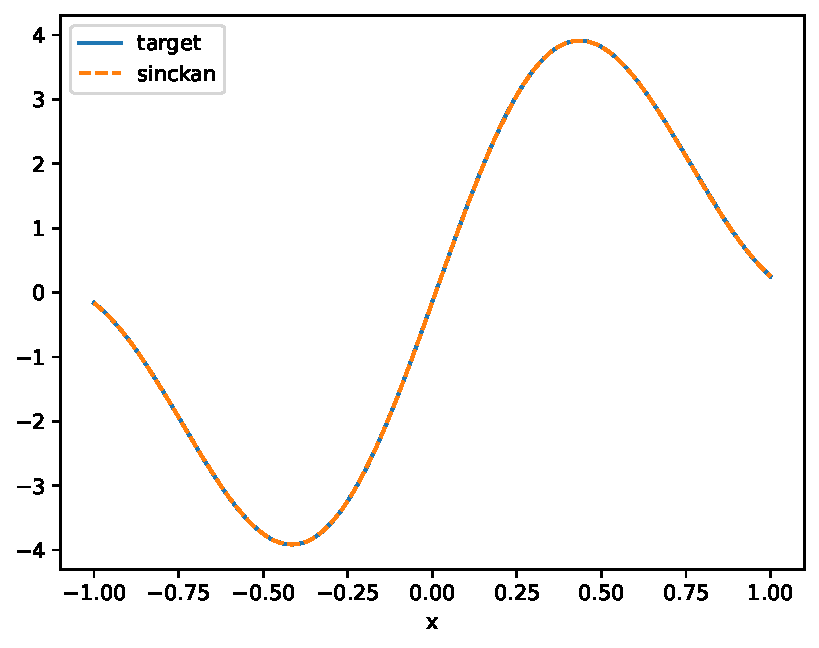
\includegraphics[width=0.4\linewidth]{ThesisFigs/cd_2_8_1.pdf}} %width==0.329
\subfigure[\label{2_8_6} $h_0=2.0, N=8, M=6$]{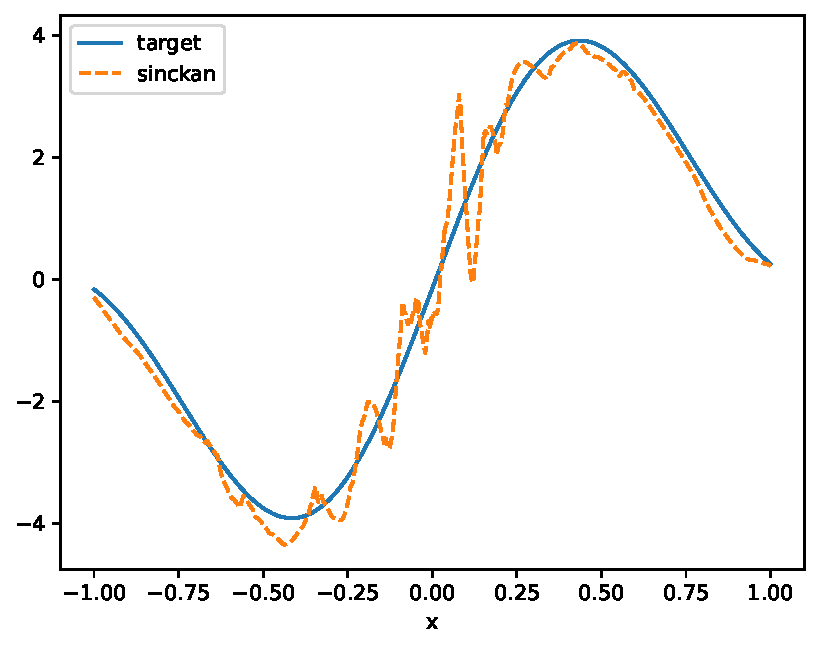
\includegraphics[width=0.4\linewidth]{ThesisFigs/cd_2_8_6.pdf}}
\subfigure[\label{10_8_1} $h_0=10.0, N=8, M=1$]{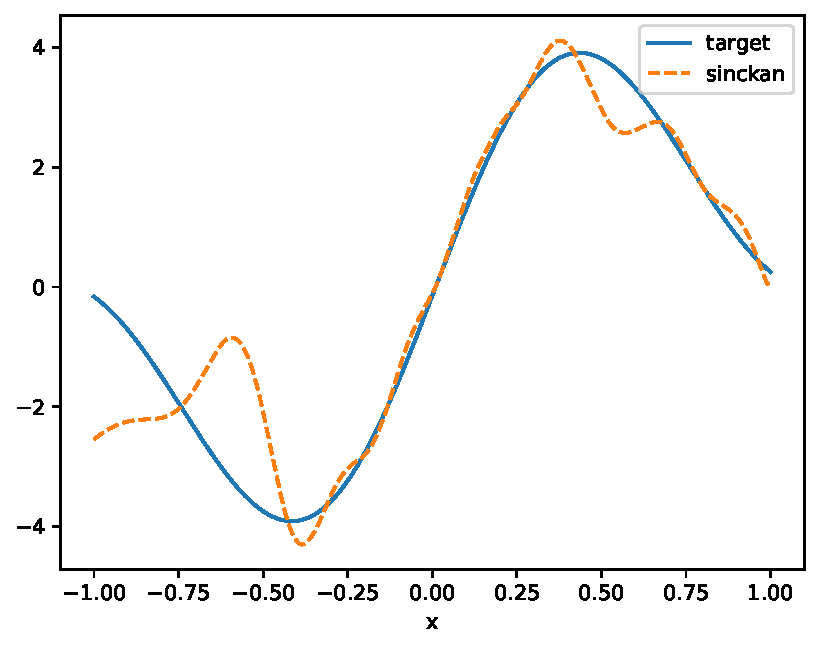
\includegraphics[width=0.4\linewidth]{ThesisFigs/cd_10_8_1.pdf}}
\subfigure[\label{2_100_6} $h_0=2.0, N=100, M=6$]{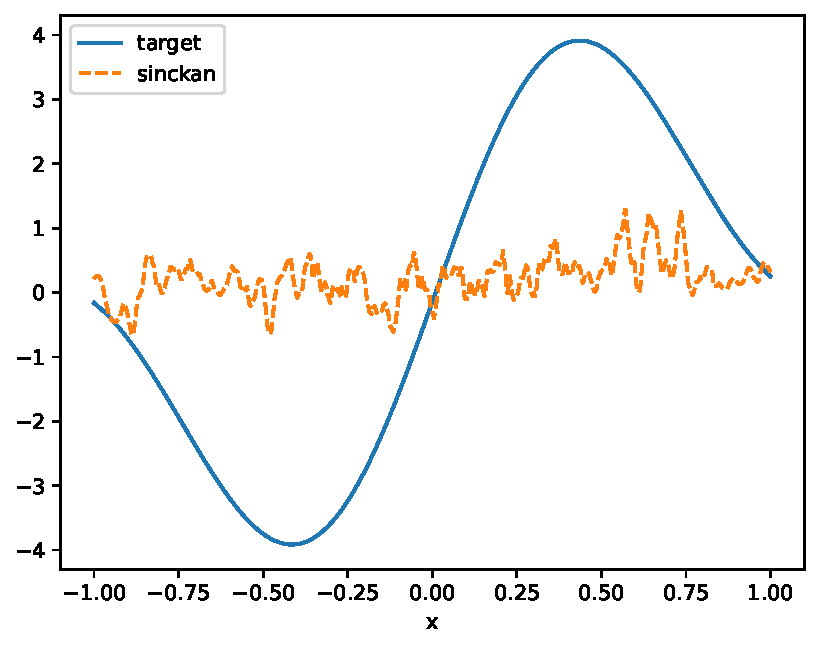
\includegraphics[width=0.4\linewidth]{ThesisFigs/cd_2_100_6.pdf}}
\caption{\cref{2_8_1} solve \cref{eq:cd} accurately. However, SincKANs have oscillations after either increasing $M$ (\cref{2_8_6}) or increasing $h_0$. \cref{2_100_6} shows that with the same hyperparameters used in approximation, SincKAN becomes extremely inaccurate due to the violent oscillations.}
\label{fig:oscillation}
\end{figure}
\section{Metrics}
In this research, two primary metrics were employed. For interpolation purposes, the RMSE metric was adopted from KAN~\cite{liu2024kan}, defined as:
\begin{equation}
\mathrm{RMSE}=\sqrt{\frac{1}{N}\sum_{i=1}^{N}(y_i-\hat{y}_i)^2};
\end{equation}
For PIKANs, the relative L2 error, commonly utilized in PINNs, was implemented:
\begin{equation}
    \mathrm{Relative L2}=\frac{\|\boldsymbol{y}-\hat{\boldsymbol{y}}\|_2}{\|\boldsymbol{y}\|_2},
\end{equation}
where $y$ represents the target value and $\hat{y}$ denotes the predicted value.

% ------------------------------------------------------------------------

%%% Local Variables: 
%%% mode: latex
%%% TeX-master: "../thesis"
%%% End: 

\include{Appendix2/appendix2}

% use this line if you want bibs to appear in table of contents:
\backmatter
\addcontentsline{toc}{chapter}{Bibliography} 

\bibliography{References/references} % put your favourite Bibtex archive references here
\bibliographystyle{plainnat}

\end{document}

